\documentclass[fontsize=12pt, a4paper,pagesize=auto,toc=listof,twoside,chapterprefix=false,appendixprefix=true,open=right]{scrbook}


% Pacotes usados
% from KOMA
\usepackage{scrhack} % evita warning do lst listings
\usepackage{indentfirst}
\usepackage{needspace}
\usepackage{outlines}
% usa mais interfaces de saída
%  solution for the error “no room for a new \write” (This is a deep magic over TeX)
%\usepackage{morewrites}
%\morewritessetup{allocate=10}

% texto em português
% https://tex.stackexchange.com/questions/13172/detect-which-tex-engine-is-used
\usepackage{iftex}
\ifpdftex
	\typeout{^^J *** PDF MODE ***}
	\usepackage{cmap} % Make PDF files searchable and copyable
	\usepackage[utf8]{inputenc}
	\usepackage{scrwfile}
\fi
\ifluatex
	\typeout{^^J *** LuaLaTeX MODE ***}
\fi

\usepackage[brazilian]{babel}
%\usepackage[T1]{fontenc}

% FONTES USADAS!!!
\usepackage{lmodern}
\usepackage{marvosym}
% bbding tem cross também
\let\Cross\relax
\usepackage{bbding}

\usepackage[dvipsnames]{xcolor}

%%%%%%%%%%%%%%%%%%%% l3packages
% This collection contains implementations for aspects of the LATEX3 kernel, dealing with higher-level ideas such as the Designer Interface
% pacotes i3packages
% frações mais flexíveis
\usepackage{xfrac}
% provides a high-level interface for declaring document commands
\usepackage{xparse}

%%%%%%%%%%%%%%%%%%% FIM l3packages




% to use \currenttime
\usepackage{datetime}

% avoid pdf warning messages from pdflatex
%\pdfminorversion=6



%\usepackage{kpfonts}

% melhor typesetting
\usepackage{microtype}

%
%\usepackage{showframe}
%\usepackage[a4paper]{geometry}
%\usepackage[a4paper,top=2cm,left=2cm,right=2cm,bottom=2cm]{geometry}
%Letra  de início de parágrafo
%\usepackage{lettrine}

% controle melhor dos captions
% Captions e SUB FIGURAS (subcations resolve esse problema melhor)
\usepackage[centerlast,font={small}]{caption}
\setlength{\captionmargin}{1cm}
\usepackage{subcaption}

% usa o H em imagens
%\usepackage{float}

% pacote para gerenciar quotes pequenos e grandes
%tem o comando \enquote
\usepackage[style=brazilian]{csquotes}
% from the manual
\renewcommand*{\mkcitation}[1]{ #1}
% magic for better quotes
%https://latex.org/forum/viewtopic.php?t=5444
\newenvironment*{smallquote}
   {\quote\footnotesize}
   {\endquote}
\SetBlockEnvironment{smallquote}

% Makeindex
% Não está gerando os índices
\usepackage{imakeidx}
\makeindex
\renewcommand{\printindex}{%
  \clearpage
  \phantomsection
  % Comente a linha abaixo se não quiser no sumário:
  % \addcontentsline{toc}{chapter}{Índice Remissivo}
  % Você pode usar \chapter{Índice Remissivo} aqui se quiser com número:
  \markboth{Índice Remissivo}{Índice Remissivo}%
  \input{\jobname.ind}%
}

% vamos usar o biblatex, recomendação
%citestyle=alphabetic,bibstyle=authortitle
\usepackage[ citestyle=authoryear,articlein=false,
style=ext-authoryear-comp
,natbib=true]{biblatex}


% fix "acedido" por algo mais razoável
% fiz "e alli" por "et al."
%\DefineBibliographyStrings{portuguese}{%
%  urlseen={Disponível em}
  %,andothers={et al.},andmore={et al.}
%  }
 % USE and other no campo author para forçar et al.
%\bibliographystyle{plainnat} %without url for book entries
% https://tex.stackexchange.com/questions/445858/changing-reference-style-in-biblatex
%https://tex.stackexchange.com/questions/10682/suppress-in-biblatex
% http://linorg.usp.br/CTAN/macros/latex/contrib/biblatex-contrib/biblatex-ext/biblatex-ext.pdf


%add document elements like a bibliography or an index to the Table of Contents
%\usepackage[nottoc,notlof,notlot]{tocbibind}

\usepackage{graphicx}

% novas keys de trim e valign (usado em vários
% tabelas com imagens
% export permite usar no includegraphics (exporta para ele)
\usepackage[export]{adjustbox}
%\graphicspath{ {./imagens/} }

% The Tkiz packages
\usepackage{pgf,tikz}
\usepackage{mathrsfs}
\usepackage{icomma}


\usepackage{comandos/pgf-pie}
\usepackage[]{tikz-3dplot}
\usetikzlibrary{fadings}

\usetikzlibrary{calc}
\usetikzlibrary{math}
\usetikzlibrary{shadows}
\usetikzlibrary{patterns}
\usetikzlibrary{automata}
\usetikzlibrary{positioning}
\usetikzlibrary{topaths}
\usetikzlibrary{intersections}
\usetikzlibrary{matrix}
\usetikzlibrary{mindmap}

\usetikzlibrary{datavisualization}
\usetikzlibrary{datavisualization.formats.functions}

\usetikzlibrary{arrows}
\usetikzlibrary{arrows.meta}

\usetikzlibrary{shapes}
\usetikzlibrary{shapes.arrows}
\usetikzlibrary{shapes.symbols}
\usetikzlibrary{shapes.geometric}

\usetikzlibrary{decorations}
\usetikzlibrary{decorations.shapes}
\usetikzlibrary{decorations.pathmorphing}
\usetikzlibrary{decorations.text}
\usepgflibrary{decorations.pathreplacing}
\usepgflibrary{decorations.markings}
\usepgflibrary{decorations.footprints}
\usepgflibrary{decorations.fractals}

\usepackage{pgfplots}
\usepackage{pgfplotstable}
\pgfplotsset{compat=1.14}





%\usetikzlibrary{3d}



% esse parametro evita
% que o texto seja separado da imagem
% e facilita (muito) tratar o tamanho
\usepackage[inkscapelatex=false]{svg}

%controla onde ficam os floats
% não queremos que pulem uma entrada
% usa o commando \FloatBarrier
\usepackage[section]{placeins}

% para addlinespace e toprule
\usepackage{array}
\usepackage{booktabs}
\usepackage{multirow}
\usepackage{multicol}

% permite novos tipos de colunas em Tabelas
% e ainda uma definição dinâmica
\usepackage{tabularx}
\newcolumntype{T}{>{\centering \arraybackslash}X}

% icons do CC, tem comandos conjuntos
\usepackage{ccicons}
% http://linorg.usp.br/CTAN/fonts/ccicons/ccicons.pdf

%%%%%%%%%%%% ENUMITEM configurado
\usepackage{enumitem}
% queremos menos espaço entre os itens de uma lista
\setlist{nosep}
% criando uma check-box list
\newlist{todolist}{itemize}{2}
\setlist[todolist]{label=$\square$}
% https://tex.stackexchange.com/questions/13463/specifying-bullet-type-when-using-itemize#
% o normal é \circle - e * (muito feio)
%https://texblog.org/2008/10/16/lists-enumerate-itemize-description-and-how-to-change-them/
\renewcommand{\labelitemi}{$\bullet$}
\renewcommand{\labelitemii}{$\circ$}
\renewcommand{\labelitemiii}{$\diamond$}
\renewcommand{\labelitemiv}{$\circle}
% colocando . entre 1a para ficar 1.a
% nos \ref para \labels
% https://tex.stackexchange.com/questions/288407/no-dots-in-the-cross-reference-to-an-item-from-enumerate/288412#288412
% I want dots
\makeatletter
\renewcommand\p@enumii{\theenumi.}
\renewcommand\p@enumiii{\theenumi.\theenumi.}
\makeatother
%%%%%%%%%%%% ENUMITEM END

\usepackage{fancyvrb}

% Controlar a Marca Dagua
%\usepackage{draftwatermark}
%\SetWatermarkText{DRAFT}
%\SetWatermarkScale{5}
%\SetWatermarkColor[gray]{0.90}

\usepackage{amsmath}
\usepackage{amssymb}
\usepackage{amsfonts}
\usepackage{amsthm}
%,exercise}
%\numberwithin{Answer}{chapter}
%\numberwithin{Exercise}{chapter}

% para os exercícios
\usepackage{exsol}
\renewcommand{\exercisename}{Exercício}
\renewcommand{\exercisesname}{Exercícios}
\renewcommand{\solutionname}{Solução}
\renewcommand{\solutionsname}{Soluções}
\renewcommand{\seriesname}{Série}



% minicontent
%https://tex.stackexchange.com/questions/430594/use-minitoc-with-koma-script-scrbook
\usepackage{etoc}
\newcommand{\chaptertoc}[1][Conteúdo]{
	\etocsettocstyle{\addsec*{#1\\\rule{\textwidth}{0.4pt}}}
	{\bigskip}
	\etocsettocdepth{1}
	\localtableofcontents
}


% para caixas legais
\usepackage{tcolorbox}

%para underline que quebra linha
% usar \uline
% o normalem significa manter o \emph como é
% senão ele é alterado para underline
\usepackage[normalem]{ulem}

% Títulos mais legais
%\usepackage[Bjornstrup]{fncychap}
%\usepackage{titlesec}
%\titleformat{\chapter}[hang]{\Huge\bfseries}{\thechapter\hsp\textcolor{gray75}{|}\hsp}{0pt}{\Huge\bfseries}

%Para usar casos de uso, verificar no capítulo
%comandos copiados da rede
\usepackage{comandos/usecases}

% Usando listagens
\usepackage{listings}
\lstset{extendedchars=true,basicstyle=\ttfamily,
		inputencoding=utf8,
            literate=%
            {ã}{{\~{a}}}1
            {á}{{\'{a}}}1
            {â}{{\^{a}}}1
            {à}{{\`{a}}}1
            {é}{{\'{e}}}1
            {è}{{\`{e}}}1
            {ê}{{\^{e}}}1
            {î}{{\^{i}}}1
            {í}{{\'{i}}}1
            {ô}{{\^{o}}}1
            {ó}{{\'{o}}}1
            {õ}{{\~{o}}}1
            {û}{{\^{u}}}1
            {ú}{{\'{u}}}1
            {ç}{{\c{c}}}1
            {Ç}{{\c{C}}}1
            {Ã}{{\~{A}}}1
            {À}{{\`{A}}}1
            {Â}{{\^{A}}}1
            {Á}{{\'{A}}}1
            {É}{{\'{E}}}1
            {Ê}{{\^{E}}}1
            {Î}{{\^{I}}}1
            {Í}{{\'{I}}}1
            {Ó}{{\'{O}}}1
            {Ô}{{\^{O}}}1
            {Õ}{{\~{O}}}1
            {Ú}{{\'{U}}}1
            }

\renewcommand{\lstlistlistingname}{Lista de Programas}
\renewcommand{\lstlistingname}{Lista de Programas}


\usepackage{wrapfig}

\usepackage{etoolbox} 
\usepackage{pdfpages}
\usepackage{setspace}

% para poder usar url
\usepackage{url,xurl}
\usepackage[hidelinks]{hyperref}

% lista de URLS
\newwrite\urllistfile
\immediate\openout\urllistfile=urllist.aux

\let\oldurl\url
\renewcommand{\url}[1]{\myurl{#1}}
\newcommand{\expurl}[2]{\myeurl{#1}{#2}}

\newcommand{\myurl}[1]{%
  \oldurl{#1}%
  \begingroup
    \edef\tempurl{#1}%
    \immediate\write\urllistfile{\noexpand\urllistentry{\tempurl}}%
  \endgroup
}

\newcommand{\myeurl}[2]{%
  \oldurl{#1}%
  \begingroup
    \edef\tempurl{#1}%
    \immediate\write\urllistfile{\noexpand\eurllistentry{\tempurl}{#2}}%
  \endgroup
}

\newcommand{\urllistentry}[1]{\item \oldurl{#1}}
\newcommand{\eurllistentry}[2]{\item \textbf{#2}: \oldurl{#1}}

\newcommand{\listofurls}{%
  \immediate\closeout\urllistfile
  \begin{itemize}
    \input{urllist.aux}
  \end{itemize}
}


% Comandos criados

% star - cannot contain \par (see https://tex.stackexchange.com/questions/1050/whats-the-difference-between-newcommand-and-newcommand)
\newcommand*{\gxdefine}[1]{\textbf{#1}\index{#1}}
\newcommand*{\gxdefineplus}[2][]{\textbf{#2 #1}\index{#2@\textit{#2}\ifx#1\empty\else!\textit{#1}\fi}}

\newcommand{\Excel}{Excel\texttrademark}
\newcommand{\ExcelScale}{0.4}
\newcommand{\furl}[1]{\footnote{\url{#1}}}
\newcommand{\feurl}[2]{\footnote{\expurl{#1}{#2}}}

% can´t remember what it does
\makeatletter
\DeclareRobustCommand*{\escapeus}[1]{%
    \begingroup\@activeus\scantokens{#1\endinput}\endgroup}
\begingroup\lccode`\~=`\_\relax
    \lowercase{\endgroup\def\@activeus{\catcode`\_=\active \let~\_}}
\makeatother

%% DESENHA CUBOS!
\newcommand{\drawbox}[5]{
    \pgfmathsetmacro \angle {30}
    \pgfmathsetmacro \xd {{2/3*cos(\angle)*#5}}
    \pgfmathsetmacro \yd {{2/3*sin(\angle)*#5}}
    \pgfmathsetmacro \x {{#1-#5+(#2-#5)*(\xd)*#5}}
    \pgfmathsetmacro \y {{#3-#5+(#2-#5)*(\yd)*#5}}

    \draw[fill=#4] (\x,\y) -- (\x+#5,\y) -- (\x+#5,\y+#5) -- (\x,\y+#5) -- cycle;

    \draw[fill=#4] (\x,\y+#5) -- (\x+\xd,\y+#5+\yd) -- (\x+#5+\xd,\y+#5+\yd) -- (\x+#5,\y+#5) -- cycle;

    \draw[fill=#4] (\x+#5,\y+#5) -- (\x+#5+\xd,\y+#5+\yd) -- (\x+#5+\xd,\y+\yd) -- (\x+#5,\y) -- cycle;
}

% desenha linhas malucas
\newcommand\irregularline[2]{%

%  let \n1 = {rand*(#1)} in  +(0,\n1)

  \foreach \a in {0.0,0.1,...,#2}{
    let \n1 = {rnd*(#1)} in
    -- +(\a,\n1)
  }
}  % #1=seed, #2=length of horizontal line

\setlength{\parskip}{.5em}

% scrbook permite mudar - o tipo de documento que estou usando
% e corrigir o erro
%Package tocbasic Warning: number width of figure toc entries should be
\DeclareTOCStyleEntry[numwidth=45pt]{tocline}{figure}
\DeclareTOCStyleEntry[numwidth=45pt]{tocline}{section}
\DeclareTOCStyleEntry[numwidth=45pt]{tocline}{subsection}


% comentários nas margens com alinhamento que faz sentido
%https://tex.stackexchange.com/questions/411939/marginpar-text-alignment/417276#417276
\newcommand{\alignedmarginpar}[1]{%
    \Ifthispageodd{%
        \marginpar{\raggedright\small #1}}{%
        \marginpar{\raggedleft\small #1}}%
    }


% Marcas usando bbding ou outro pacote
\newcommand{\gxok}{\textcolor{green}{\CheckmarkBold}}
\newcommand{\gxnot}{\textcolor{red}{\XSolidBold}}


% https://tex.stackexchange.com/questions/32683/rotated-column-titles-in-tabular
% cria um comando para rodar os headings das tabelas
% e acertar o tamanho das colunas,
% parametros rotacao (op) tamanho(opcional) e texto (mandatório)
% precisa do xparse
\NewDocumentCommand{\gxrot}{O{90} O{1em} m}{\makebox[#2][l]{\rotatebox{#1}{#3}}}%


\newcommand{\gxibfcolor}{NavyBlue}
\newcommand{\gxibbcolor}{White}


\newenvironment{gxwinfobox}[2][r]%
{%
\begin{wrapfigure}{#1}{0.5\textwidth}%
\begin{tcolorbox}[title=\textbf{\Info #2},colframe=\gxibfcolor,colback=\gxibbcolor]%
}%
{%
\end{tcolorbox}%
\end{wrapfigure}%
}%


\newenvironment{gxinfobox}[1]
{%
\begin{tcolorbox}[title={\Large\Info\ }\textbf{#1},%
colframe=\gxibfcolor,colback=\gxibbcolor, sharp corners=uphill]%
}%
{%
\end{tcolorbox}%
}%


\newcommand{\gxcwinfobox}[3][r]{\begin{gxwinfobox}[#1]{#2}#3\end{gxwinfobox}}

\NewDocumentCommand{\whybox}{m+m}{
    \begin{tcolorbox}[title=\textbf{Por que #1?},colframe=blue!75!black,%

        colback=white,fonttitle=\bfseries,halign=center]%
        \protect#2
\end{tcolorbox}}







\addbibresource{bibs/bibguiadoorientado.bib}
\addbibresource{bibs/refs.bib}

% \usepackage{draftwatermark}
% \SetWatermarkText{DRAFT}
% \SetWatermarkScale{5}


\title{Guia Pragmático para a Pós-Graduação}
\subtitle{Dicas do campo de batalha para você que quer terminar o mestrado ou o doutorado}
\author{Geraldo Xexéo}
\date{\today~\currenttime}


\makeindex

\begin{document}

\maketitle


\chapter*{Licença}


Este texto é distribuído com uma licença Creative Commons - Atribuição - NãoComercial - Compartilha Igual 4.0 Internacional.




\begin{center}
    \ccbyncsa
\end{center}

Você tem o direito de:
\begin{itemize}
    \item \textbf{Compartilhar} -- copiar e distribuir o material em qualquer suporte ou formato.
    \item \textbf{Adaptar} -- remixar, transformar, e criar a partir do material.
\end{itemize}

De acordo com os termos seguintes:
\begin{itemize}
    \item \textbf{Atribuição} -- Você deve dar o crédito apropriado, prover um link para a licença e indicar se mudanças foram feitas. Você deve fazê-lo em qualquer circunstância razoável, mas de nenhuma maneira que sugira que o licenciante apoia você ou o seu uso.
    \item \textbf{NãoComercial} --Você não pode usar o material para fins comerciais.
    \item \textbf{CompartilhaIgual} -- Se você remixar, transformar, ou criar a partir do material, tem de distribuir as suas contribuições sob a mesma licença que o original.
    \item \textbf{Sem restrições adicionais} -- Você não pode aplicar termos jurídicos ou medidas de caráter tecnológico que restrinjam legalmente outros de fazerem algo que a licença permita.
\end{itemize}

Mais informações podem ser encontradas em \url{https://creativecommons.org/licenses/by-nc-sa/4.0/deed.pt_BR}
\vspace*{\fill}
\begin{center}

    \Huge

    \textit{
    ``…We choose to go to the moon.
    We choose to go to the moon in this decade and do the other things, not because they are easy, but because they are hard, because that goal will serve to organize and measure the best of our energies and skills, because that challenge is one that we are willing to accept, one we are unwilling to postpone, and one which we intend to win, and the others, too. ''}

    \Large

    Discurso de John F. Kennedy

    Rice University Stadium

    12 de setembro de 1962

\end{center}
\vspace*{\fill}



\frontmatter
\tableofcontents
\listoffigures
\listoftables

\mainmatter

\chapter{Este Texto}

Este texto vem direto do campo de batalha para você.
Não é um texto sobre metodologia científica. Não vou ficar ensinando normas ou listando as regras de acentuação em português. Não vou ensinar um método preciso. Não vou escrever aqui uma receita de bolo, mas sim dar uma fotografia geral do que é importante, e do que não é importante, para alcançar o objetivo: defender a dissertação ou a tese e ser aprovado.

Este texto foi originalmente criado para os \textbf{meus alunos}, mestrandos e doutorandos em Engenharia de Dados e Conhecimento (EDC) do Programa de Engenharia de Sistemas e Computação (PESC) da Coppe/UFRJ. 

Fiz agora uma nova versão, onde as regras do PESC estão em caixas separadas ao longo do texto, e também em um capítulo no fim do texto. Ao ver uma regra do PESC, lembre que seu programa pode ter uma parecida.

Atualmente esse texto é dedicado a todos os alunos de pós-graduação, e útil para orientados de Trabalho de Conclusão de Curso (TCC). Cada aluno pode viver uma realidade diferente, mas certos princípios básicos sempre serão mantidos.

De agora em diante vou usar apenas o termo tese, querendo dizer tanto uma dissertação de mestrado quanto uma tese de doutorado. Alunos de projeto final ou trabalho de conclusão de curso podem também se aproveitar deste texto.

Se você não é meu aluno, espero que possa também aproveitar um pouco da minha visão. 



\section{As Três Partes deste Guia}

Este guia foi estruturado em três partes, cada uma abordando aspectos fundamentais da jornada de orientação acadêmica. Ele foi construído com base na experiência direta de orientação ao longo de décadas e procura oferecer conselhos práticos, realistas e — acima de tudo — aplicáveis.

A primeira parte é dedicada às pessoas envolvidas no processo: o orientador, o orientado e as demais partes interessadas. Aqui se discutem as expectativas mútuas, os tipos de alunos, os estilos de orientação e a importância da convivência acadêmica. Mais do que regras, esta parte oferece reflexões sobre papéis, responsabilidades, conflitos e acordos tácitos e explícitos que permeiam essa relação essencial para o sucesso do projeto de tese.


A segunda parte se volta ao processo em si. Aborda práticas recomendadas, armadilhas comuns, hábitos de trabalho, critérios de escolha do tema, estratégias de escrita e desafios metodológicos. Também discute o ecossistema da pós-graduação — da universidade às agências de fomento — e os ritos de passagem que marcam a trajetória do mestrado ou doutorado. O objetivo aqui é fornecer ao orientando ferramentas concretas para navegar, com autonomia e consistência, pelos desafios do percurso.

Por fim, a terceira parte apresenta indicações específicas sobre como trabalhar comigo, o autor e orientador. Trata-se de um conjunto de orientações personalizadas, que refletem não apenas um estilo de orientação, mas também uma forma de organizar o trabalho, colaborar em publicações e conduzir projetos conjuntos. Essa parte é particularmente relevante para meus alunos, mas pode inspirar outros orientadores e orientandos a refletirem sobre como tornar mais eficaz e transparente sua própria relação de trabalho.

Não esqueça de ler os apêndices, que buscam trazer uma abordagem mais leve a algumas questões levantadas.


\chapter{Princípio Fundamental do Orientado}
\label{chap:pfo}
\index{Princípio Fundamental do Orientado}


\gxatencao{O princípio fundamental do orientado é que ele é o único responsável pela sua tese ou dissertação.}

O orientador já fez a sua tese, já passou em um concurso para professor e está aí para ajudar o orientado, mas a responsabilidade final com esforço, qualidade e prazos é do candidato ao título.

Durante o desenvolvimento da dissertação ou tese, o orientador é um guia que, dependendo do perfil, das disponibilidades ou do relacionamento que cria com o orientado, pode interferir mais ou menos no trabalho deste último, fornecer mais ou menos recursos, dar a ideia fundamental ou não, porém nunca será o responsável por realizá-lo.

Para seguir este princípio, o aluno, e candidato ao título, deve ter a consciência de todas as suas obrigações e direitos; para isso, deve, logo ao entrar no curso, encontrar e ler:

\begin{outline}
\1	O regulamento do seu curso.
\2	No momento as principais informações relevantes para os alunos da COPPE podem ser encontradas no site da Coppe, na seção \textbf{Espaço do Aluno} \url{https://coppe.ufrj.br/espaco-do-aluno/}. Lá está o
a regulamentação original\furl{https://coppe.ufrj.br/wp-content/uploads/2024/06/Alunos_a_partir_2017.1.pdf} e ainda vários documentos e decisões adicionais.
\1	As decisões tomadas após o regulamento e que são válidas para o seu curso
\1	Todos os seus prazos, incluindo
\2	A duração da bolsa
\2	A data esperada pelo programa de pós-graduação e data máxima permitida para:
\3	Terminar os créditos.
\3	Defender os exames de qualificação, seminários de qualificação ou similares.
\3	Apresentar e defender a dissertação ou tese.
\1	Os contratos e documentos que assina, principalmente em relação à bolsa, e as responsabilidades que dela advêm.
\1	Conhecer as notas necessárias para poder concluir o curso
\2	Na COPPE, a média deve ser B (2,0) ou maior.
\end{outline}

\chapter{Nós}

\begin{center}
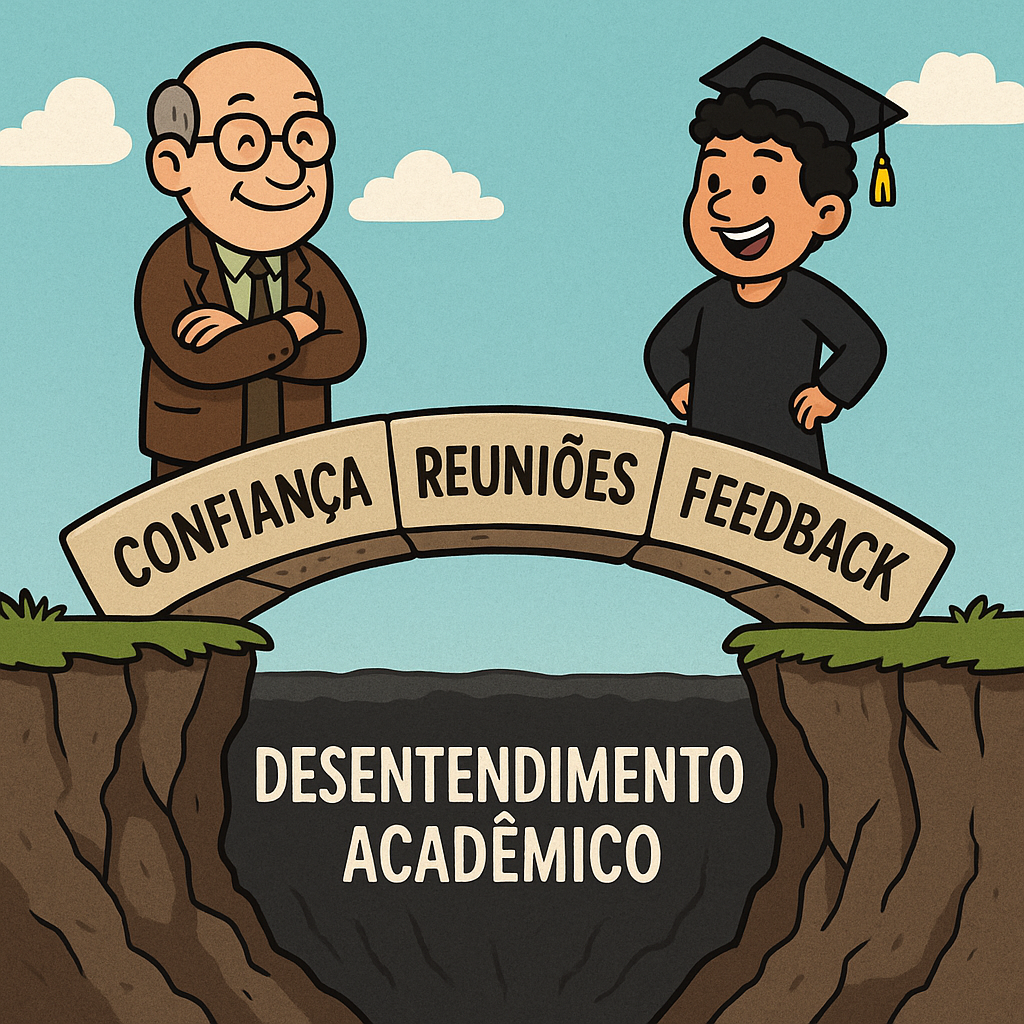
\includegraphics[width=0.5\linewidth]{Images/nos.png}    
\end{center}
\vspace{0.5cm}

\section{Eu - O Autor e Um Orientador}

Eu sou professor de graduação e pós-graduação, doutor, engenheiro e orientador em teses, dissertações e projetos finais. Tenho 30 anos de experiência nessa atividade. Para chegar a essa posição eu também tive que defender um projeto final e uma tese\footnote{Eu nunca fiz um mestrado!}. Vi também amigos meus passarem por essa experiência. Acompanho meus alunos e alunos de outros professores.

Falo com diferentes perspectivas. A primeira é de um autor genérico, descrevendo como as coisas são, ou como deviam ser. A segunda é como orientador, descrevendo como eu quero que as coisas sejam. A terceira é como professor do Programa de Engenharia de Sistemas da Coppe/UFRJ, trazendo informações específicas dessa instituição.

A maior parte do texto é atemporal. Muito pouco mudou nas relações humanas nos últimos 40 anos em que estou na academia, desde minha graduação. A tecnologia mudou a forma, mas a essência é a mesma. A parte relacionada a regras específicas sempre sofre com o tempo. Se você pegou este texto depois de 2025, talvez haja uma versão mais nova disponível. 



\section{Você – O Leitor e Um Orientado}

Você deve ser muito inteligente, já que se candidatou e foi aceito para a pós-graduação. Deve ter também um bom currículo e estar acostumado a ter sucesso em sua vida acadêmica e, se não for recém-formado, na profissional.
Nada disso será o fator determinante para você acabar sua tese e obter seu título.

Para defender sua tese você precisa escrever e, entre outras opções, construir um artefato, fazer um protótipo, executar experimentos computacionais ou uma pesquisa de campo.

Isso se resume a \textbf{trabalhar com dedicação}. A inteligência pode ajudar e até mesmo diminuir seu esforço, mas é a dedicação que fará com que você alcance seus objetivos.

Vários alunos inteligentes não conseguem obter seus títulos. Isso acontece porque eles caem em várias armadilhas, muitas causadas pela própria inteligência, ou o otimismo de achar que pode fazer tudo rápido. Porém, é raro ver um aluno dedicado que não defenda sua tese, inclusive com brilhantismo.

Esse texto pretende indicar alguns caminhos, apontar algumas armadilhas e auxiliá-lo, de várias formas, a se preparar para essa difícil tarefa.


\chapter{O Tema da Tese}

A tese obrigatoriamente tem que ter um assunto, que deve ser escolhido no início do trabalho. Essa escolha é importante e deve ser feita com cuidado, de modo a que permita ao candidato crescer academicamente, contribuir para o conhecimento e, ao mesmo tempo, evitar dissabores.

\gxatencao{O aluno deve se identificar com o tema de tese escolhido.}

Você não vai conseguir acabar uma tese da qual não goste do tema desde o início do seu trabalho. Mesmo gostando do tema inicialmente, é possível que no fim da tese você não queira ver mais o tema “nem pintado”, o que não é bom, mas pelo menos você terminou a tese.

O tema deve ser escolhido com muito cuidado. Primeiro, deve ser de seu interesse, praticamente uma paixão. Segundo, deve ser de interesse do orientador. Finalmente deve ser do interesse da comunidade científica.

Alguns temas, mesmo sendo de interesse pessoal, não interessam a ninguém.

Ou por já estarem resolvidos, ou por não serem ainda percebidos, ou pior, porque não têm valor científico, ou não têm valor na comunidade científica a que o candidato pertence.

Normalmente se faz um plano de tese no início. Esse plano nem sempre é seguido, pois com o tempo entendemos melhor o problema, suas formas mais genéricas ou mais específicas, e alterações de rota são feitas.

Não se preocupe muito no início, no primeiro ano do doutorado, ou nos três primeiros meses de pesquisa no mestrado, se seu tema é incerto. Seu objetivo deve ser fixado nesse prazo, mas o mais importante é entender o contexto do tema e os problemas importantes a serem resolvidos. Depois, nos próximos 2 ou 3 anos, você irá em direção a fechar a tese.

Para escolher o tema, é importante que você escolha cadeiras que tenham relação com assuntos de seu interesse. Não escolha cadeiras pela facilidade ou pelo horário disponível, escolha cadeiras que lhe ajudem a escolher e estudar temas de seu interesse.

% TODO: \usepackage{graphicx} required
\begin{figure}[hbt]
    \centering
    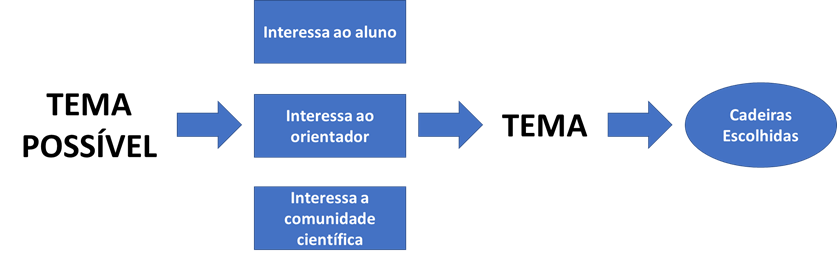
\includegraphics[width=0.9\linewidth]{Images/escolhatemacadeiras}
    \caption{Escolhendo tema e cadeiras. Fonte: o autor}
    \label{fig:escolhatemacadeiras}
\end{figure}


\section{O que é uma Contribuição Original}

Um dos requisitos da tese de doutorado é possuir uma contribuição original.

Eu confesso que contribuição original não é uma definição muito clara. Vamos analisar, então, o que é uma contribuição.

A professora Marta Mattoso diz que :
\begin{itemize}
\item	“Uma contribuição é um resultado que pode ser útil para outras pessoas.”
\item	“O resultado é uma novidade e não poderia ser afirmado sem o desenvolvimento da tese.”
\end{itemize}

Ou seja, uma contribuição pode se algo como encontrado na lista a seguir, levemente ordenada da maior para a menor e de forma não exaustiva.
\begin{enumerate}
\item	A solução de um problema em aberto;
\item	Uma melhoria comprovada a alguma prática da área;
\item	A proposta de uma metodologia, método ou processo que resolva um problema do mundo real, com uma abordagem científica;
\item	Aplicar uma prática da área em uma área de aplicação, de maneira não trivial;
\item	A investigação de um problema que descobre novas evidências na área;
\item	A criação de sistemas complexos envolvendo várias práticas até antes isoladas, com um resultado científico palpável;
\item	A comparação e análise de diferentes soluções computacionais para o mesmo problema, com consequente desenvolvimento de solução que as agregam de alguma forma;
\item	O levantamento de uma história, ou o estudo de casos, que trazem contribuição original para o entendimento de como algo aconteceu ou acontece, sempre de acordo com metodologias reconhecidas;
\item	A criação de novas bases de dados que podem servir para outros trabalhos.
\end{enumerate}

Porém, ao contrário de outras áreas, no Programa de Engenharia de Sistemas e Computação, e em toda COPPE, não é considerada uma contribuição;
\begin{itemize}
    \item 	Fazer a compilação de dados ou informações já existentes (como a criação de um review da área);
    \item	Desenvolver aplicações convencionais com software disponível amplamente;
    \item 	Desenvolver protótipos com tecnologia amplamente conhecida e divulgada.

\end{itemize}

Veja que a tese tem que comprovar a contribuição. Não basta dizer que algo é bom e original, é importante poder provar que é melhor (mesmo que dentro de alguns casos) e que não há outro resultado igual, ou ainda que abre um caminho novo de pesquisa.

\section{Como encontrar uma Contribuição}

Normalmente em uma tese de computação existe um problema, uma solução e uma comprovação ou validação da solução.

Assim, uma tese pode apresentar contribuições nessas três áreas. Lidando com o problema, podemos encontrar novos problemas ainda não tratados e modelar de formas diferentes problemas já tratados.

Na solução, podemos aplicar técnicas já existentes em problemas ainda não tratados com elas ou inventar novas técnicas. Finalmente, podemos trabalhar arduamente nas técnicas de comprovação de nossos resultados, principalmente quando esses resultados são experimentais ou empíricos\footnote{Em soluções teóricas é necessário provar que a solução é verdadeira, porém isso normalmente é parte da própria solução. Porém, existem teses teóricas que apresentam novas formas, mais simples, de provar um teorema já provado}.

O importante é ter um problema bem claro. Esse problema pode já ter sido proposto antes, ou pode ser levantado. Uma maneira de levantar problemas é estudar soluções já existentes e ver quando elas falham, ou que lacunas elas têm.

Listar as falhas ou lacunas de uma situação atual é um bom método de descobrir onde você pode trabalhar. As lacunas podem ser elencadas, algumas podem ser selecionadas, e toda a tese construída em torno desse conceito.

Muitos alunos querem começar pela solução, algo do tipo “quero usar a técnica X”. Esse não é um bom caminho, apesar de já ter funcionado para algumas pessoas. Porém, o que acontece normalmente é que o aluno fica com uma solução a procura de um problema e não tem como comprovar a qualidade ou a utilidade de sua solução.


\section{Pensando sua Tese}

Várias técnicas podem ser usadas para você pensar sua tese.

Algumas técnicas são muito úteis. Uma delas é a \gxdefine{5W2H}, responder as perguntas: Why, What, Who, When, Where, How e How Much. Essa é das técnicas mais gerais e mais úteis. Principalmente se perguntar “Por que estou fazendo isso” e “Quem vai ser beneficiado” permitem justificar plenamente o trabalho de sua tese, fazendo com que ela não fique perdida em um contexto vago.  A Figura \ref{fig:5w2h} mostra algumas perguntas possíveis nessa técnica.

% TODO: \usepackage{graphicx} required
\begin{figure}[hbt]
    \centering
    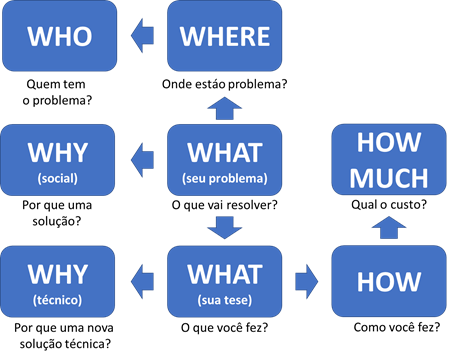
\includegraphics[width=0.7\linewidth]{Images/5w2h}
    \caption{Perguntas que devem ser respondidas antes de iniciar uma tese. Fonte: do autor.}
    \label{fig:5w2h}
\end{figure}




Algumas teses atuais têm proposto lacunas no estado da arte, e a partir dessas lacunas geram questões de pesquisa, que por sua vez podem gerar objetivos gerais e específicos. Esse é outro bom quadro teórico para trabalhar.

Entre meus alunos, o uso da \gxdefine{Design Science Research} (\gxdefine{DSR})\citep{Pimentel2020} também fornece caminhos para pensar sua tese . Eu estou me tornando cada vez mais um adepto dessa metodologia, dessa forma de fazer Ciência, que é realizada por meio de vários processos mais detalhados. Ou seja, não existe um método científico DSR, ele é mais uma filosofia de trabalho que fornece parâmetros para estabelecer um método específico.

Outra técnica possível, é desenhar um \gxdefine{Project Model Canvas}\footnote{\url{http://www.projectmodelcanvas.com/}} . Essa é uma proposta de José Finocchio Júnior e tem uma representação visual interessante, apresentada na Figura \ref{fig:pmc}.

% TODO: \usepackage{graphicx} required
\begin{figure}
    \centering
    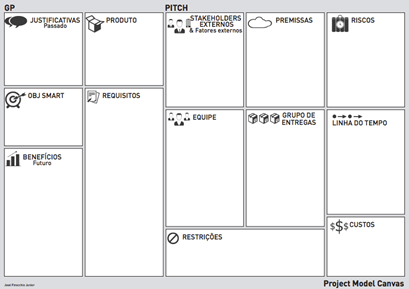
\includegraphics[width=0.7\linewidth]{Images/PMC}
    \caption{Representação do Project Model Canvas de José Finocchio Júnior (CC:BYNOND)}
    \label{fig:pmc}
\end{figure}


\section{Como descrever o que é a tese}

Algumas coisas são importantes para você definir sua tese.

Primeiro, você tem que \textbf{conhecer um problema} e o \textbf{estado da arte da solução} do problema. Se seu orientador trabalha com o problema, você ainda tem que conhecer bem o trabalho que ele tem feito, para entrar realmente no grupo.

Segundo, é interessante que você consiga dar um \textbf{valor} a esse problema\footnote{Você pode ouvir uma aula sobre valor em \url{https://youtu.be/aOQQHGzC-YE}, ou ler o capítulo sobre valor escrito em \url{https://github.com/xexeo/MaterialEducacional}} . O valor pode ser econômico, como a diminuição de um custo, pode ser um valor acadêmico, como um teorema em aberto a muito tempo, ou pode ser outra forma de valor, como social ou histórico. Uma visão rápida de Valor, típica da Engenharia de Software, é procurar 3 coisas: aumentar o faturamento (benefícios), reduzir custos e melhorar serviços.

Terceiro, você deve ter uma \textbf{proposta de abordagem ao problema}. Isto significa que você deve entender caminhos possíveis para resolvê-lo e ter uma ideia das técnicas que pretende adotar.

Todas essas coisas podem ser descritas de várias formas, tanto ao longo do trabalho em apresentações como no texto final. Algumas abordagens mais tradicionais que outras.

\section{A descrição da tese na introdução}

Na introdução da sua tese deve existir uma descrição do que ela é e que deixe o leitor totalmente ciente do que vai encontrar durante a leitura.

Por exemplo, é importante \textbf{definir o problema} que a tese trata. Esse problema deve ocorrer dentro de um \textbf{contexto}. Também deve ficar claro o \textbf{objetivo} da tese. Esse objetivo pode ser dividido em \textbf{questões de pesquisa}, que devem levar gradativamente ao objetivo, ou pode gerar \textbf{conjecturas} que precisam ser comprovadas ou pelo menos validadas, já que certas conjecturas são difíceis de serem comprovadas de forma absoluta, devido a incluírem, por exemplo, aspectos do comportamento humano.

Costumamos, reservar o termo \textbf{hipótese para conjecturas que podem ser provadas com experimentos} que incluem uma hipótese nula, por meios estatísticos, ou provada, ou negada, por meio de um teorema. Chamar de hipótese, no corpo da tese, algo que não pode ser comprovado dessa forma, cria uma expectativa errada no leitor. Caso não haja uma comprovação formal, devemos evitar o termo hipótese e usar outros como conjecturas ou questões de pesquisa.

Podem ser necessárias também a elaboração de uma ou mais \textbf{premissas}, que são afirmações consideradas válidas a priori para sua tese. Premissas não são questionadas ao logo da tese, e sim assumidas como válidas. Claro que se espera que as premissas tenham alguma evidência, ou seja, não sejam facilmente falseáveis.


\chapter{O Seu Objetivo}

\begin{center}
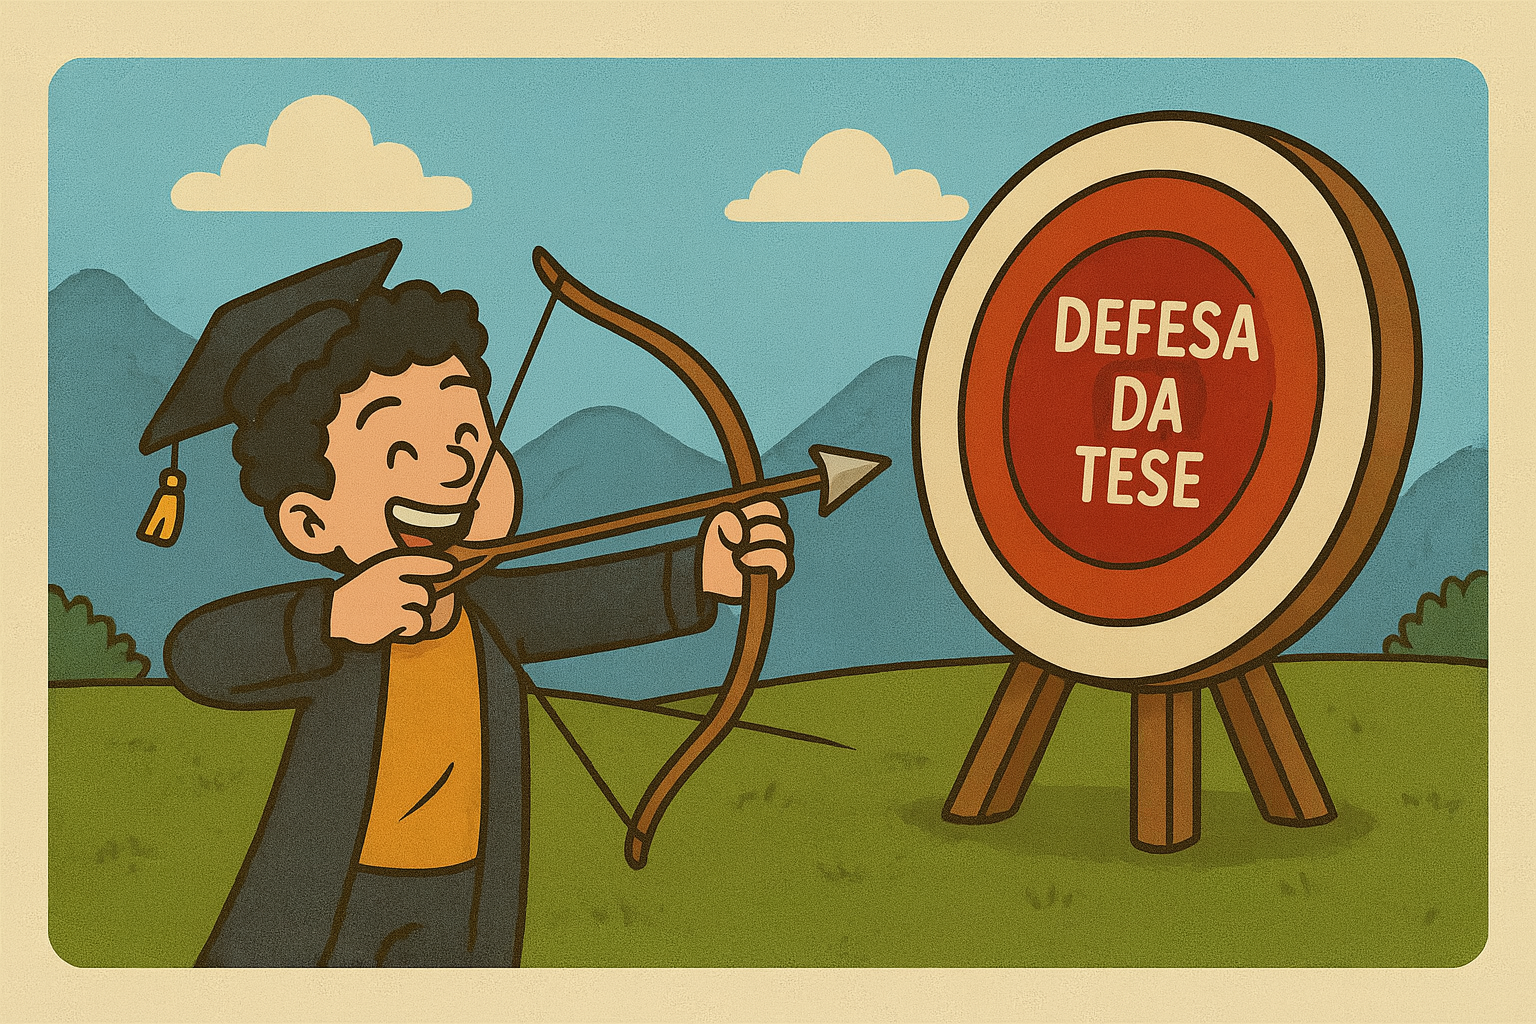
\includegraphics[width=0.5\linewidth]{Images/objetivoseta.png}    
\end{center}
\vspace{0.5cm}


Vamos deixar bem claro:

\gxatencao{O seu objetivo é defender a tese!}

Uma tese \textbf{não} é um trabalho completo que vai dar a melhor solução do mundo para o problema mais importante que existe.

\CoppeWay{Como é na Coppe}{
Na Coppe, uma tese tem objetivos definidos da seguinte forma :
\begin{itemize}
\item	``A Dissertação de Mestrado deverá demonstrar a aptidão do candidato para desenvolver atividades de pesquisa no tema escolhido e configurar uma contribuição significativa para o conhecimento na área correspondente''
\item	``A Tese de Doutorado deverá apresentar características de originalidade, demonstrando a aptidão do candidato para desenvolver atividades de pesquisa, e configurar uma contribuição significativa para o conhecimento nas áreas escolhidas de pesquisa''
\end{itemize}
}

Sua tese tem que ser uma \textbf{contribuição} para a área e, no caso do Doutorado, apresentar características de originalidade. É comum que uma tese de mestrado já apresente essas características, mas não é necessário.

Além disso, sua tese deve \textbf{acabar dentro do prazo}.

Alguns ditados que recolhi entre amigos orientadores e orientados deixam bem clara a importância de terminar a tese:

\begin{center}
``Tese não se termina, se entrega.''

``Tese boa é tese que acaba.''

``Você quer salvar o mundo ou tirar o título?''
    
\end{center}

Essas, e outras variações, são necessárias porque é comum o autor da tese achar que precisa ``resolver o problema do mundo'' ou que deve fazer uma tese perfeita. Isso é impossível, pois a tese está limitada em tempo.

Uma característica importante sobre teses de Doutorado: ao contrário do que muitos alunos pensam, uma tese que deixe muitos caminhos abertos é muito boa. Se isso acontece, o novo doutor é capaz de construir sua carreira, pelo menos inicialmente, resolvendo os problemas que ele mesmo descobriu ou tornou solucionáveis.

A professora Ana Regina Cavalcanti da Rocha costuma dizer:

\gxatencao{A Tese de Doutorado não é o último trabalho da vida de aluno, mas sim o primeiro trabalho da vida de pesquisador.}




\chapter{As Partes Interessadas na Sua Tese}

Toda tese é um projeto. As boas práticas de projeto sugerem que você levante, no início do projeto, e controle e gerencie, ao longo do projeto, as partes interessadas no projeto.
Mas o que são as partes interessadas? Não seriam apenas você, ou você e seu orientador, as únicas partes interessadas?

Uma parte interessada é qualquer pessoa ou grupo que afete ou seja afetado pela sua tese, de verdade ou por percepção. A partir dessa definição, vemos que existem muito mais partes interessadas.

Por exemplo, todos que se relacionam de maneira afetiva no dia a dia com você serão afetados pela sua tese, e alguns afetarão. 
Sua disponibilidade de tempo e atenção passará a ser dividida com a tese. 
Vários momentos que antes eram livres passarão a ser ocupados com pesquisas, leituras, programação, experimentos e outras atividades. 
Isso pode afetar os seus relacionamentos e você deve prestar atenção para que não prejudique fortemente sua vida pessoal.

Gostaria de contar o caso de um doutorando que mantinha um escritório fechado, para evitar que fosse desorganizado. 
Seu filho pequeno, ao ver a porta aberta, entrou e fez a maior confusão, porque tinha ``raiva'' do pai ficar no escritório e não com ele. Em outro exemplo, um mestre recém-formado ouviu um ultimato de sua esposa: ``Se você for fazer doutorado eu peço o divórcio''. Ele é doutor hoje em dia, e está feliz no segundo casamento.

O \textbf{principal interessado normalmente é você}. Mas não apenas o você científico ou profissional, mas o você ``completo''. Não só você afeta a tese, pois o sucesso dela depende do seu esforço, mas será também afetado por ela. O stress da pesquisa, da defesa, da dívida constante de trabalho, já causou problemas de saúde, física e mental, para muitos. Estudos mostram alarmantes  graus de depressão entre alunos de pós-graduação~\citep{walker2015}.

O \textbf{orientador é outra parte interessada óbvia}. Todo orientador realmente quer que todos orientados defendam sua tese. Porém, são também guardiões da qualidade do diploma, logo, querem que a tese seja boa. Um bom orientador deve reprovar um aluno que não alcance os padrões acadêmicos de sua instituição, mas isso sempre é feito com desgosto. Mais de uma vez compartilhei com colegas a sensação de tristeza de ter um aluno que prometia resultados, mas não consegue, por um motivo ou outro, atingir um padrão de qualidade que garanta sua defesa.

Os membros da banca darão a palavra final da aprovação da sua tese. A tese deve atender a padrões de qualidade, de honestidade científica, e eles são a barreira final. Muitas vezes, seu orientador sinalizará: você precisa atender aos padrões da banca, tem que ser capaz de convencer o leitor.

Depois desses grupos básicos, temos outras partes interessadas. Seu programa, os órgãos de fomento, a universidade, a sua comunidade científica e a sociedade em geral. Todos eles devem ser atendidos. 

Cabe então, a você, ao iniciar sua tese, pensar em como vai atender a todos. Seu orientador pode ajudar.

\section{Sua Família}
Família e tese são quase tão incompatíveis como trabalho e tese. A tese exige atenção. Nem sempre esposa, marido, filhos e filhas estão preparados para perder parte do tempo da atenção que lhes é normalmente dispensada para uma atividade intrinsecamente solitária.

A primeira coisa a lembrar é que você precisa também dar atenção à família. Se decidir estudar todo domingo, por exemplo, saia com as crianças de manhã cedo e só depois comece a estudar. 

Aproveite os momentos de descanso para fazê-los com sua família. 

Antes de começar uma tese, converse com sua família. Explique a necessidade de tempo, apoio e compreensão. Se necessário, deixe acordado desde o início que espaço de tempo será ``integral'' da família e não pode ser tocado. 

A hora de dormir com as crianças, o dever de casa, o cinema no sábado, o jantar romântico, tudo pode ter seu lugar se houver alguma organização de sua parte. 

\section{Seu Trabalho}

Se você trabalha, está em desvantagem. 
Em primeiro lugar, a pós-graduação não foi pensada, principalmente no Brasil, para quem trabalha, mas sim para quem se dedica exclusivamente a pesquisa. 

Além disso, mesmo que seu empregador ou seu chefe tenha prometido a liberação, deixá-lo realizar seu sonho, ele realmente precisa que você trabalhe e ganhe dinheiro para a empresa. Isso significa que todas as promessas do seu empregador serão esquecidas com o tempo.

Algumas organizações, principalmente as públicas, liberam você para fazer sua tese. Para sermos justos, uma liberação de 4 anos, 2 para o mestrado, atende às necessidades de qualquer aluno (mesmo que você tenha mais prazo). É vital acabar a tese antes do final da liberação. Voltar para o trabalho sem terminar a tese não só atrapalha o fim dela como pode ser considerado por seus colegas como uma espécie de ``derrota'', atrapalhando sua carreira. A pior situação possível seria você voltar e nunca acabar a tese! 

Também é comum que o aluno seja liberado para as cadeiras, mas não para o desenvolvimento da tese. Isso é um mau sinal. Caso seja liberado para as cadeiras apenas, tente pelo menos que o tempo de estudo seja incluído nessa liberação. Normalmente, aconselhamos o aluno a considerar que o tempo de estudo para uma cadeira é, no mínimo, duas vezes maior que o tempo de aula. Isso significa que, para cada hora de aula, você teria que ter mais duas horas liberadas, totalizando três horas! Você pode colocar algumas dessas horas de estudo a noite ou no fim de semana, mas não todas.

É importante que você tenha por escrito todas as promessas da companhia, assinadas por uma pessoa com autoridade sobre seu chefe imediato, pelo Diretor de Recursos Humanos ou pessoa comparável.
Se você pertence a uma instituição com atenção curta, que toda hora muda de foco, seus problemas serão maiores. Quanto menor a sua empresa, maiores serão seus problemas. Se seu cargo envolve viagens constantes, seus problemas serão tão grandes que talvez seja impossível você realizar seus cursos ou defender a sua tese.

Se você trabalha na Universidade, então certamente terá mais chances e muito menos problemas. Se você pretende arranjar bicos durante o curso, procure trabalhos ligados à educação.Lembre que, a princípio, investimento na pós-graduação tem muito mais valor que o salário que você deixa de ganhar. 

\section{Os Órgãos de Fomento}

Se você ganha uma bolsa de algum órgão de fomento, como FAPERJ, CAPES e CNPq, você tem a responsabilidade legal de acabar a tese. 
Apesar de não ter sido a prática por muito tempo, atualmente há investigações e pedidos de restituição dos valores pagos como bolsa para alunos que não terminaram suas teses e não possuem uma justificativa.

Atenção também à taxa de bancada. Ela não é um adicional à tese, mas uma verba destinada a gastos na sua pesquisa e que devem ser comprovados. Você terá que prestar um relatório final e pode ser auditado.





\chapter{Que Tipo de Aluno Você É?}

A tese é um projeto de uma só pessoa. Seu orientador, por mais interesse que tenha no assunto, não vai fazê-la por você. Isso seria, inclusive, antiético e ilegal.


A responsabilidade é basicamente sua e o sucesso será prioritariamente seu. Logo, a pessoa mais importante nesse projeto é você, pois é a única que pode completá-lo. Compreender a si mesmo é um fator importante nesse processo. Entender suas características, sejam elas positivas ou negativas, ajudará a alcançar seu objetivo.



\section{Conhecendo Suas Necessidades}

Antes de começar um projeto de mestrado ou doutorado, o aluno deve estar ciente de suas necessidades, limitações, restrições, capacidades e habilidades. Tudo isso deve ser levado em conta na sua preparação e mesmo na escolha se é o momento certo para realizar essa empreitada.

Em especial, quero chamar a atenção às necessidades. Um trabalho de extrema repercussão é o estudo de Maslow  sobre a hierarquia de necessidades das pessoas\footnote{Esse trabalho também foi muito criticado, mas certamente podemos utilizá-lo para exemplificar o fato de que você tem que estar bem em vários sentidos para ter a calma necessária para fazer sua tese.}. Ele é facilmente compreendido a partir da “pirâmide de Maslow”, que apresento na Figura \ref{fig:maslow}.

\begin{figure}
	\centering
	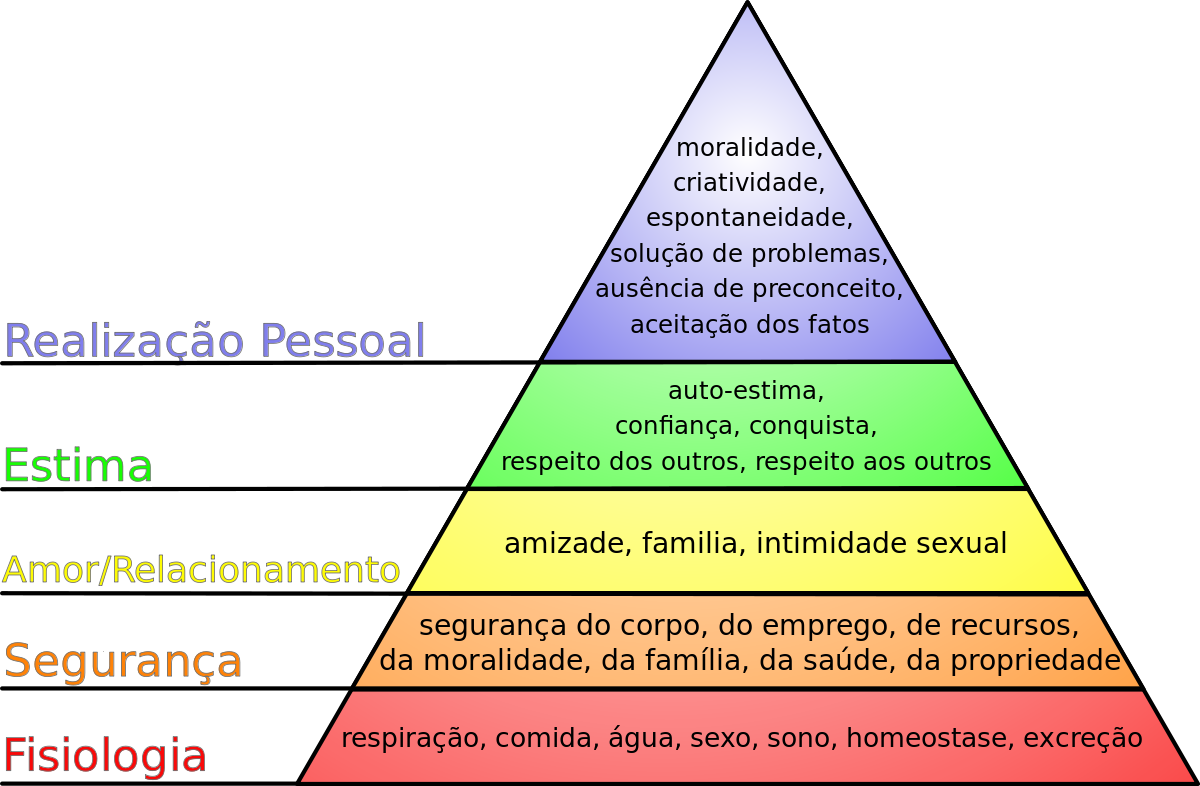
\includegraphics[width=0.7\linewidth]{Images/1200px-Hierarquia_das_necessidades_de_Maslow.svg}
	\caption{A pirâmide de Maslow.}
	\label{fig:maslow}
\end{figure}


Como se pode ver na Figura \ref{fig:maslow}, as necessidades são divididas em grupos e um grupo serve de base para todos os grupos superiores. Assim, as necessidades de realização pessoal (como fazer uma tese) são dependentes de todas as outras. 

Desse modo, podemos concluir que, para fazer uma pós-graduação, você deve garantir antes que tenha uma “boa base na pirâmide”. Isso significa garantir sua saúde, o modo de se manter, seus relacionamentos e sua autoestima.

Mesmo que você tenha começado sua dissertação ou tese em uma situação ideal, o longo prazo desse projeto, de 2 a 5 anos, implica em mudanças tanto no ambiente à sua volta quanto na sua própria vida. Alunos se casam, têm filhos, ficam doentes, se curam, precisam de mais dinheiro, se separam, trocam de emprego, tudo pode mudar nesse espaço de tempo.
Podemos citar como exemplo de acontecimento totalmente inesperado, e que afetou a todos em 2020/2021, a epidemia da Covid-19. Quantas vidas não foram mudadas? O impacto na vida dos mestrandos e graduandos foi muito variado e colocou um grande desafio para orientandos, orientadores e as instituições.

Voltando a pirâmide, ela indica que qualquer problema em uma camada inferior afeta diretamente a camada superior. Você deve estar consciente dessa estrutura e saber que problemas de qualquer tipo sempre afetarão seu rendimento na camada do topo, seja ocupando seu tempo, seja ocupando sua mente. Cabe ao aluno perceber e controlar o grau desse efeito e, quando necessário, interagir com o orientador.

Por isso não hesite em procurar seu orientador e avisá-lo do que está acontecendo com você. Mesmo que ele não possa ajudá-lo no problema específico, ele compreenderá e tentará ajudar no que for possível. 
Exemplos típicos de coisas que acontecem na vida de um aluno: um novo emprego ou uma situação de desemprego, troca de chefes que afeta a liberação ou o interesse da empresa, doenças mais ou menos graves consigo ou com parentes, perda de acesso aos dados prometidos por alguém, gravidez, casamento, etc.

O orientador não é um sargento empurrando você em uma marcha forçada. Ao contrário, ele é o guia que evita que você se perca em uma exploração. Ele está ali para auxiliá-lo nos percalços do caminho, até mesmo para dizer que está na hora de parar e tentar em outra expedição. 
Uma relação aberta com o orientador é uma das mensagens que quero passar nesse texto. Ela vai facilitar sua vida e chegar ao seu objetivo.

\section{Que Tipo de Aluno Você É?}

Uma maneira de compreender a si mesmo é conhecer estereótipos comuns das pessoas e ver até que ponto você se encaixa nesses estereótipos. 


Existem muitos tipos de alunos. Um orientador, com o tempo, desenvolve sua fórmula pessoal para tratar cada um deles. No texto a seguir, apresentarei alguns estereótipos. Raramente um aluno segue fielmente um desses estereótipos, mas eles servem como referência.


Apresentarei também algumas maneiras de se autoavaliar. Fique certo que muitos irão avaliar seu desempenho, principalmente seus orientadores. Muitas vezes receberá críticas, algumas justas, outras não. Entender a si mesmo e entender por que as pessoas o percebem de certa forma o ajudará a progredir.


Os alunos têm diferentes graus de dependência, ou independência, do orientador. A maioria dos alunos passa, durante a tese, por vários desses “graus”. Vamos analisar como funcionam os alunos estereotipados: o totalmente dependente e os totalmente independentes.


\subsection{O estereótipo independente}


O aluno totalmente independente é normalmente uma pessoa com interesses bem específicos. Escolhe um tema que o orientador pode auxiliar, mas não é necessariamente especialista. Sua relação de orientação é feita a partir da comunicação de tempos em tempos, ao orientador, do que está fazendo. Nessa conversa, tem sempre uma proposta de solução quando apresenta um problema e procura conhecer a opinião do orientador. 


Tive bons alunos desse tipo. Talvez todos eles tenham se envolvido, em alguma parte da tese, em problemas.


Um dos problemas que podem acontecer é que esse aluno, por se manter distante do orientador, tanto fisicamente quanto em relação ao tema de tese, não consiga imprimir um ritmo adequado sozinho. Isso se torna mais crítico quando o aluno tem alguma dificuldade pessoal grave e acaba “sem tempo” de informar o orientador.


\gxatencao{O aluno deve informar imediatamente ao orientador de qualquer problema pessoal que esteja dificultando ou impedindo seu progresso.
}

Principalmente com problemas emocionais, de saúde e financeiros graves, com si mesmo ou com sua família, o aluno deve informar o orientador e tomar com ele decisões como continuar trabalhando, ou suspender o trabalho ou até mesmo, e muito raramente, abandonar a tese. 

\gxatencao{O importante é que o aluno traga o problema ao orientador antes de criar um problema com seu prazo ou com suas avaliações}.


Outra coisa que pode acontecer é o aluno independente achar que o orientador o abandonou. Ele nunca fala com o orientador e, nas raras vezes que fala ou tenta falar, o orientador está muito ocupado. O orientador pode achar que o aluno o abandonou também, já que o aluno nunca o procura. Na verdade, pode ser que ambos tenham razão. 


Se houver alguma comunicação entre os dois e essa comunicação for clara, e a iniciativa do aluno for boa, a tese deve ser concluída. Se o aluno perder a iniciativa, o orientador terá trabalho para recolocá-lo nos trilhos, talvez não consiga. Se a comunicação for pequena o aluno corre o risco de querer fazer coisas demais e não acabar a tese ou fazer tudo errado, pois não sabe algum detalhe importante que o orientador já estudou.


No limite, alguns alunos desprezam a orientação, acham que o orientador não sabe o que está fazendo, ou simplesmente não ligam para a orientação.


Isso é péssimo. O orientador é mais experiente que o aluno e, se não tem a percepção localizada do assunto, por estar estudando menos o tema que o aluno naquele instante, tem a percepção generalizada bem mais apurada que a do aluno. Por isso que um é orientador e o outro aluno.


Um ditado típico da minha família é:


\gxatencao{O diabo não é perigoso por ser mais inteligente. 
O diabo não é perigoso por ser mais forte. 
O diabo é perigoso porque é mais velho.}


O orientador é mais velho, ou pelo menos está há mais tempo na área. Ou seja, o aluno independente tem muitas características boas, porém tem um risco muito alto.


\subsection{O estereótipo dependente}


Do outro lado do espectro, existe o aluno totalmente dependente. Esse aluno não faz nada sem perguntar ao orientador. Não tem ideias próprias. Desenvolve trabalhos a partir da orientação do orientador e fazendo implementações segundo algoritmos definidos pelo orientador. Nunca perde o contato. 


Supondo que esse aluno é competente, ele é um aluno de risco baixo. Tem grandes chances de acabar a tese, porque faz tudo que o orientador manda e o orientador deve saber em que direção vai à tese. 


Os riscos em relação a esse aluno ocorrem se orientador estiver em uma fase muito criativa, mas sem foco ou sem tempo. 


Outro risco importante é o aluno não se identificar com a tese, porque foi escolhida pelo orientador. 


\subsection{O aluno real}


Se você olhar as descrições acima com cuidado vai perceber algo estranho: o aluno independente, supostamente o melhor aluno, é o que corre mais riscos. Isso acontece porque tanto a construção de uma dissertação ou tese quanto a orientação são processos. Quanto mais o orientado faz parte do processo, mais chances têm que terminá-lo de forma satisfatória.


Obviamente, nenhum aluno é totalmente independente ou dependente. Pessoalmente, tive boas relações com alunos em vários pontos do espectro. O importante é que o aluno permaneça em contato com o orientador. 


Aviso aos orientados que é o aluno que se mantém em contato com o orientador, não o inverso. É o aluno que deve procurar, marcar reuniões, trazer o trabalho. É o orientado que deve esperar pelo orientador na porta de sua sala. O orientador possui vários alunos e tarefas, dificilmente consegue controlar a frequência de cada um. Lembre-se, você é um dos alunos de seu orientador, enquanto seu orientador é o único que você tem.


\gxatencao{O aluno deve se manter em contato com o orientador.}


Uma história pessoal: quando queria falar com meu orientador sozinho, sem interrupção, eu pegava uma carona. Era a única forma de ter um “tempo só para mim”. E nem sempre dava certo.


\subsection{Como se avaliar quanto à independência}


Tente responder as seguintes perguntas:
\begin{itemize}
	\item Eu converso com meu orientador com uma frequência fixa?
	\item Quantas vezes por mês eu converso com meu orientador?
	\item Meu orientador é capaz de dizer em que ponto eu estou na minha tese?
	\item Meu orientador é capaz de falar sobre minha tese?
\end{itemize}





\chapter{Hábitos e Práticas}


Ao ingressar em um programa de pós-graduação, o aluno deixa de ser apenas um receptor de conhecimentos e passa a atuar como um produtor de saberes. Esse processo exige o desenvolvimento de hábitos e práticas que sustentem uma formação científica sólida, crítica e produtiva. Neste capítulo, discutimos duas dessas práticas fundamentais: a leitura e a escrita.

Não se trata apenas de habilidades técnicas, mas de atitudes intelectuais que definem a postura do pesquisador diante do conhecimento. Ler é muito mais do que coletar informações — é construir um repertório teórico, compreender o estado da arte, dialogar com outros autores e localizar sua própria pesquisa dentro da comunidade científica. Escrever, por sua vez, é articular ideias com clareza, defender argumentos com coerência e contribuir para o avanço da ciência por meio da comunicação dos resultados.

Estes hábitos, quando cultivados com disciplina e intencionalidade, tornam-se ferramentas poderosas para a construção da autonomia acadêmica. O objetivo deste capítulo é apresentar orientações práticas para que o aluno desenvolva essas competências com consciência de sua importância e com estratégias que possam ser incorporadas à rotina de trabalho acadêmico.


\section{Ler}


A leitura é a única forma do candidato a um título alcançar a maturidade necessária para defendê-lo. Muitos alunos têm uma boa ideia e acreditam que realizá-la e descrevê-la caracteriza uma tese. Isso não é verdade. 


\gxatencao{O aluno deve ler.}


Uma tese tem que ser colocada no contexto científico atual e comparada com os trabalhos já realizados sobre o assunto ou sobre temas similares ou análogos. Deve ficar claro, na tese, qual a colaboração que o trabalho traz à ciência. Obviamente, só é possível fazer isso se o aluno tiver um conhecimento da área, que deve ser, na maior parte das vezes, até mesmo superior ao conhecimento do orientador.


Quando o aluno não lê o suficiente isso fica muito claro para o orientador. Há uma falta de capacidade de argumentação, uma falta de base teórica para o trabalho. Um dos principais sinais de maturidade que um orientador percebe é a capacidade de argumentação baseada em evidências científicas.


É importante notar que não basta ler, mas é necessário ler publicações atualizadas (além dos textos clássicos da área).


Se você achar que está lendo pouco, ou se seu orientador reclamar disso, aqui estão algumas dicas:

\begin{outline}	
\1	Levante uma lista de congressos e revistas relativas à área de sua tese.
\2	Faça um mix com o máximo possível de publicações da área específica com publicações importantes da área mais geral.
\1	Obtenha os últimos cinco anos desses congressos e revistas.
\1	Liste todos os artigos disponíveis que possam servir para sua tese.
\1	Obtenha esses artigos.
\1	Leia os resumos e os organize de alguma forma, priorizando a leitura.
\2	Procure tutoriais e reviews para o início da leitura.
\2	Leia alguns artigos clássicos citados nos artigos obtidos.
\2 Leia os artigos específicos, com foco nos mais atuais.
\1	Mantenha o controle dessa lista e faça o acompanhamento com o orientador.
\end{outline}

A maioria dos textos de metodologia científica recomenda o fichamento dos artigos lidos. Essa prática é importante, porém não é mais necessário usar fichas. Você pode usar um banco de dados, um sistema de referência ou até mesmo um ou mais arquivos de documento, como arquivos Word. Até mesmo “Post-it” pode gerar um bom sistema de fichamento. 


\subsection{O Aluno que só lê português (e não conta ao orientador)}


Dificilmente você será aceito no mestrado se sua capacitação em inglês não permite uma leitura em ritmo razoável, porém isso pode acontecer.


Nesse caso, deixe bem claro ao orientador sua dificuldade. Esconder qualquer dificuldade de leitura ou compreensão, seja ela de inglês ou de alguma matéria específica, fará com que seu orientador avalie sua dificuldade como falta de dedicação.


O resultado é que, em vez de o orientador ajudá-lo nessa dificuldade, ele tornará as coisas cada vez mais difíceis.


Por sinal, se esse for seu caso, entre imediatamente em um curso de inglês. Qualquer melhoria, junto com a leitura de textos da área, implicará em um rendimento maior do seu trabalho. Existem cursos gratuitos ou muito baratos na universidade.


\section{Escrever}


É quase impossível seguir uma carreira acadêmica em qualquer área de sem escrever bem, pelo menos em português. 


Se você acha que escreve mal, ou se os outros acham que escreve mal, tente corrigir o mais rápido possível. Faça cursos e se esforce. Muitos alunos simplesmente acham “normal” um profissional de área técnica escrever mal. Isso demonstra uma falta de compreensão das necessidades do mundo real: apresentar e defender, de forma clara, suas ideias. 


Como diria o Chacrinha\footnote{É provável que alguns dos leitores mais novos não tenham conhecido o “Chacrinha”. Ele foi por muitos anos um apresentador de programa de auditório de muito sucesso, usando uma fantasia e utilizando bordões engraçados. Certamente foi uma das figuras mais conhecidas na TV brasileira do século XX.}: 


\gxatencao{Quem não se comunica, se trumbica}


Uma das principais indicações da educação de uma pessoa é sua capacidade de se expressar em sua língua mãe.


Ao estudante universitário, essa característica é muito desejada. Ao aluno de mestrado e doutorado, é indispensável.


Contribuição de um aluno que aprendeu a escrever.

\begin{quote}

Só consegue escrever quem consegue dizer o que pensa e quer.  Fale, diga o que pensa, conte para seu orientador suas ideias e busque clareza ao dizer.

Escreva simples.  Uma tese é, antes de qualquer coisa, uma coleção de folhas de papel com um monte de letrinhas em cima.  

Ler é, depois de falar, uma das melhores ajudas para quem quer aprender a escrever.  Ler tudo, de jornal a bula de remédio, passando por contos, poesias, história em quadrinhos, artigos e, naturalmente, uma tese ou outra de vez em quando.

Depois fica-se assim, querendo escrever em qualquer lugar, em qualquer oportunidade, em qualquer Wiki que se abra.

Desejo boa sorte a nós todos.

\textit{Bebeto}

\end{quote}

\chapter{O Orientador}



\section{A expectativa do Orientador}

O orientador espera que o aluno seja ético, trabalhador e inteligente, provavelmente nessa ordem. Esse é o parâmetro que orientadores tentam prever no processo de seleção, tanto no inicial, quando o aluno se candidata ao curso, quanto na escolha dos orientantos\footnote{No PESC os alunos são selecionados por linha e escolhem os orientadores ao longo do curso.}

A ética é necessária tanto na pesquisa quanto no relacionamento. O orientador espera que o aluno seja honesto e transparente quanto às suas atividades e resultados. Quando o aluno fiz ``eu fiz isso'' o orientador acredita. Porém, se o aluno não tem como mostrar que fez, ou não é capaz de desenvolver raciocínios e propostas sobre o que disse ter feito, o orientador começa a duvidar e o relacionamento se degrada.

O orientador espera que o aluno trabalhe. Isso significa que ele espera um fluxo de entregas periódico, de acordo com a carga de trabalho esperada implicitamente em função do tipo de matrícula (tempo integral ou parcial). 

Finalmente, o orientador espera um grau de inteligência e conhecimento razoável. A verdade é que muitos associam o título de mestre ou doutor a uma inteligência  supostamente superior, mas na verdade isso não é necessário. O que é necessário é um grau de conhecimento suficiente para trazer uma contribuição relevante, e dedicação. 

Uma outra expectativa do orientador é que o aluno seja pró-ativo e não-dependente. Leia o texto ``Mensagem a Garcia'' no autoref{chap:garcia}.

\section{O que você espera do orientador?}

No mínimo você deve exigir que o orientador seja ético e que respeite o aluno como ser humano. Práticas abusivas, apesar de serem comuns, não podem ser toleradas e devem ser denunciadas pelos canais oficiais.

Em segundo lugar, o aluno deve esperar que o orientador aloque ao seu atendimento um tempo proporcional a duas coisas:
\begin{itemize}
    \item A quantidade de alunos e outras tarefas do orientador
    \item A capacidade de resposta, ou ritmo de interação, do aluno
\end{itemize}
Isso quer dizer que um aluno que demora três meses para trazer um resultado não pode esperar que o orientador o avalie no mesmo dia. Na verdade, já conheci orientadores que tinham como norma demorar o mesmo tempo que demorou para um trabalho ser entregue para avaliar o trabalho. Há um pouco de exagero nessa regra, porém posso, como orientador, entender o porquê dessa exigência.

Assim, não se iluda, se seu orientador tem um cargo administrativo, vários projetos, muitos alunos, seu tempo será menor. Provavelmente, nesse caso, ele é um orientador experiente e seu tempo também será \textbf{melhor}, mas nem sempre isso é verdade.

O aluno também deve esperar que o orientador \textbf{oriente}, ou seja, indique caminhos para seguir e para evitar. Para isso ser bem feito, depende também da experiência do orientador, então se você escolhe um orientador muito novo, pode ter uma resposta de menor qualidade em relação a isso, mas melhor em relação a outros fatores.

Além desses avisos, a pergunta é: o que você espera do orientador? Que tal fazer uma lista, para ajudar no processo de escolha?


\section{Qual a Função do Orientador}

A função do orientador é orientar, mostrar caminhos, estimulá-lo a pesquisa, gerar problemas que você possa resolver. Ele também deve ajudar com a burocracia e com problemas relacionados à universidade. 

Não é função do orientador resolver os problemas da sua tese. Porém, ele pode, eventualmente, dar contribuições essenciais.

Alguns orientadores vão ajudá-lo a resolver problemas pessoais, provavelmente apenas com conselhos, mas não é essa sua função. Ele deve conhecer os problemas para entender a sua produtividade, mas não é sua obrigação resolvê-los. Se o faz, faz por vontade própria e solidariedade.

A relação orientado/orientador é muito variada, porém deve ser sempre cordial. Faça todos os esforços possíveis para não iniciar uma discussão pessoal com seu orientador. 

\gxatencao{O respeito é essencial}

A primeira coisa a entender é que o orientador não é orientador por ser mais inteligente que você, mas por ter mais experiência que você em uma área específica. Muitas vezes os orientadores são mais novos que os orientados e mesmo assim alcançam bons resultados. É claro que é importante que você respeite a inteligência do seu orientador, mas esse não é o fator de diferença entre orientado e orientador.

\section{Dificuldades comuns com os orientadores}


Normalmente, seu orientador o tratará com respeito, porém os seguintes problemas podem aparecer:

\begin{outline}
\1	O orientador não tem tempo para você
\1	O orientador não leu o que você escreveu
\1	O orientador não entende o que você faz
\end{outline}

\subsection{O Orientador sem tempo}


É comum um orientador ter pouco tempo disponível. Ele tem que dar aulas, participar de reuniões, orientar outros alunos e realizar atividades como pesquisa e consultoria. Você deve se adaptar ao tempo disponível de seu orientador. 

\gxatencao{O orientado deve se adaptar aos horários do orientador, não o contrário.}

Algumas desculpas são inaceitáveis pelo orientador e entre elas está que ``você não pode sair de seu trabalho nessa hora''. Afinal, você está ou não fazendo uma tese? É possível, porém, que seu orientador concorde em o orientar na casa dele, após o expediente, e, em casos excepcionais, no fim de semana. Não é o meu caso e acredito que, tirando condições excepcionais, não devia ser o caso de nenhum orientador.

Caso seu orientador tenha problemas graves na agenda, tente marcar um almoço com ele. Outra opção é conseguir um coorientador, outro professor da mesma área ou um aluno de doutorado, caso você seja aluno de mestrado. Muitos orientadores gostam de trabalhar no regime de dupla orientação.


\subsection{O orientador que não leu o que você escreveu}


Se o orientador não leu o que você escreveu é porque não teve tempo ou esqueceu. Se ao encontrar seu orientador ele não tiver lido o que você escreveu, faça um resumo mostrando o texto para ele. Raramente o orientador é ``preguiçoso'' ou ``desatento'', mas frequentemente é sobrecarregado. 


\gxatencao{Sempre leve uma cópia do trabalho que você está fazendo para as reuniões. }


Aparecer em uma reunião sem isso é demonstrar desinteresse pela reunião, falta de preparação ou, pior, que você não fez nada.

Muitos orientadores leem um texto por alto e ficam com uma ideia muito clara do que foi feito. Principalmente nos casos de revisão bibliográfica e resultados demonstrados em gráficos, o orientador pode, em 10 ou 15 minutos, ter uma ideia clara do seu trabalho e contribuir para o seu desenvolvimento. 


É importante entender que o esforço do orientador é muito relacionado ao esforço do aluno. Alguns alunos parecem frustrados porque o orientador, na segunda ou terceira vez que eles aparecem com o trabalho no mesmo estágio, não está disposto a conversar por muito tempo ou dar ideias. Essa reação não é nada surpreendente, se você não faz o seu trabalho, o orientador não tem como fazer o dele.


\gxatencao{Um processo de orientação se baseia na evolução do trabalho do orientado.}


\subsection{O orientador que não entende o que você faz}

Das três situações que citei, essa é a mais difícil de resolver.

Não é raro que um aluno desenvolva um assunto de tese que foge dos conhecimentos do orientador. Nesse caso, muitos orientadores coíbem o desenvolvimento da tese, enquanto outros buscam soluções de compromisso. Outros podem entender como uma oportunidade de abordar novas áreas. Na verdade, dependendo do assunto, a disposição do orientador pode mudar.

Uma coorientação pode, novamente, ser uma boa solução. Uma revisão bibliográfica também pode dar ao orientador as ferramentas necessárias para auxiliar no seu trabalho. Em geral, um orientador fica feliz se seu aluno sabe mais que ele sobre um assunto.


\section{Mais sobre os orientadores}


Os orientadores também passam por ciclos de alta imaginação e excessiva realidade. Muitas conversas serão ``viagens'' e outras serão ``convocações para pôr o pé no chão''. De certa forma, essa é a tarefa do orientador. Se você estiver viajando pouco, ele vai tentar desenvolver os limites da sua imaginação; se você estiver passeando no espaço sideral, ele vai tentar trazê-lo de volta para a realidade.


As conversas com o orientador devem ser plenamente documentadas, pelo aluno, mesmo que o orientador faça isso. Se os dois estiverem documentando a conversação, compare as notas no final. 


\gxatencao{O aluno deve sair de cada conversa com uma lista de itens a fazer}


Se seu orientador não criar essa lista, pergunte diretamente quais devem ser seus próximos passos ou sugira você mesmo uma lista de ações. 


Entre duas sessões de orientação, seu orientador certamente mudará de ideia. 


\gxatencao{Nunca jogue fora um trabalho anteriormente descartado}


Caso um assunto previamente descartado como ``ruim'' seja considerado ``bom'' em uma reunião posterior, verifique em suas anotações o motivo da decisão anterior e discuta-os com o orientador. Porém, tente não questionar a mudança de opinião, pois isso só vai levar a um sermão sobre a necessidade de se ter uma mente aberta e pronta para mudanças. Revise os defeitos e qualidades da opção sendo estudada e tome uma nova decisão.


Existem muitos tipos de orientadores: o viajante, o amigão, o carrasco, o executivo, o objetivo etc. Todos esses têm suas vantagens e desvantagens, cabe a você descobrir quais os defeitos do seu orientador e evitar que eles tenham má influência na sua tese. Se seu orientador tem muitas ideias, você deve ser objetivo, se seu orientador é relapso com prazos, você deve cumprir todos. Orientadores são seres humanos e têm defeitos, muitas vezes graves. 


Só você pode evitar que esses defeitos influenciem na sua tese. Quanto aos seus defeitos, fique certo de que o orientador irá apontá-los no decorrer do relacionamento, algumas vezes até de maneira um tanto rude.


\section{Confiança no orientador}


O maior desejo do orientador é que o aluno termine a tese. É quase inconcebível imaginar que um orientador não deseje que o aluno complete o mais rápido possível e da melhor forma, o seu trabalho. 

Por que falo isso com tanta certeza? Porque os professores são avaliados, parcialmente, pela capacidade de fazer seus alunos defenderem suas teses e publicarem artigos sobre elas.

Alguns alunos, porém, imaginam que o professor está contra eles. Acham que estão pedindo trabalhos impossíveis, apenas para o benefício próprio, ou pior, para atrapalhá-los.

A verdade é que cada orientador determina um nível de qualidade aceitável para o trabalho do aluno. Esse nível é compatível com as características do aluno. 
Assim, um aluno capaz de fazer ótimos programas de computador, mas péssimo em teoria, é estimulado, e cobrado, a explorar suas qualidades ao máximo e a lutar, na medida do possível e do aceitável, contra suas dificuldades.

O orientador trabalha \textbf{sempre a favor do aluno}, dentro de algumas restrições pessoais e institucionais. 
Essas restrições envolvem a área de pesquisa, a qualidade do resultado, a dedicação ao trabalho e muitos outros fatores. 
Poucas vezes um orientador reprova ou abandona um aluno.
 Ele sempre tenta ao máximo encontrar um caminho de sucesso. 
 Essa é a tarefa principal do orientador.

Uma restrição importante que todo aluno deve estar atento é que a carreira acadêmica do orientador é fortemente, se não unicamente, influenciada pela quantidade e qualidade de suas publicações. 
O orientador é um professor que tem que arcar com muitas responsabilidades: aulas, administração da faculdade, orientação e escrever artigos. 
Assim, os orientadores normalmente esperam que o orientado os auxiliem na tarefa de escrever artigos. 

Os alunos que desejam seguir carreira acadêmica devem ficar especialmente preocupados em publicar, afinal, eles também serão julgados por sua capacidade de produção de artigos.

\gxatencao{Assim, o aluno deve estabelecer uma relação de confiança e colaboração com seu orientador.}


\section{A Escolha}


A escolha do orientador é um processo bastante complicado. Alguns alunos não têm essa opção, pois são selecionados desde o início para serem orientados por um professor. 


Você pode analisar um orientador de acordo com as seguintes facetas:
\begin{enumerate}
	\item 	Compatibilidade pessoal
	\item 	Assuntos comuns
	\item 	Qualidade como orientador
	\item 	Qualidade como professor
	\item 	Qualidade como pesquisador
	\item 	Opinião pessoal
\end{enumerate}

Existem muitas maneiras de iniciar essa seleção. Normalmente você deve ter como opção os professores com qual já fez alguma cadeira ou trabalho. Seus colegas mais antigos também são capazes de dar informações sobre os professores disponíveis. Além disso, muitas vezes outros professores podem recomendar um colega, de acordo com seus objetivos como aluno.


Um conselho importante é não se assustar muito com orientadores com fama de durões. Um orientador durão pode ser um ótimo orientador e manter você nos ``trilhos certos''. Cuidado, porém, com os que têm fama de mal-educados.


\section{Problemas com o orientador}


Aconteceu! Você discutiu com seu orientador de forma irreconciliável ou se acha prejudicado fortemente. O que fazer?

Primeiro, respire. É importante parar para pensar, pois existe um registro histórico que é desfavorável a você: seu orientador já orientou diversos alunos e trabalhos, você não fez nenhuma tese.

É fato que todo relacionamento de longo prazo está sujeito a turbulências. Namoros e casamentos acabam, por que uma orientação não pode acabar? O problema é que, nesse caso, normalmente apenas um lado é prejudicado: o aluno.

Para resolver o problema, temos que pensar em um escalonamento de soluções. 

Por incrível que pareça, a primeira pessoa que pode ajudá-lo é o próprio orientador. Tente marcar outra reunião e de forma educada dizer que não consegue mais trabalhar nas condições atuais. Lembre-se que, sendo a parte mais frágil, acusar pouco vai servir a você. Seu orientador então pode se propor a buscar um novo orientador ou um coorientador. Essa solução é a mais fácil.

A seguir, caso isso não funcione, você deve caminhar lentamente pelas instâncias superiores da instituição. Na COPPE existe um chefe de linha, a coordenação acadêmica e o coordenador, dentro do Programa. No nível de diretoria ainda existe o Coordenador Acadêmico e o Conselho de Pós-Graduação e Pesquisa(CPGP).


\chapter{Dedicação Para a Tese}

\begin{center}
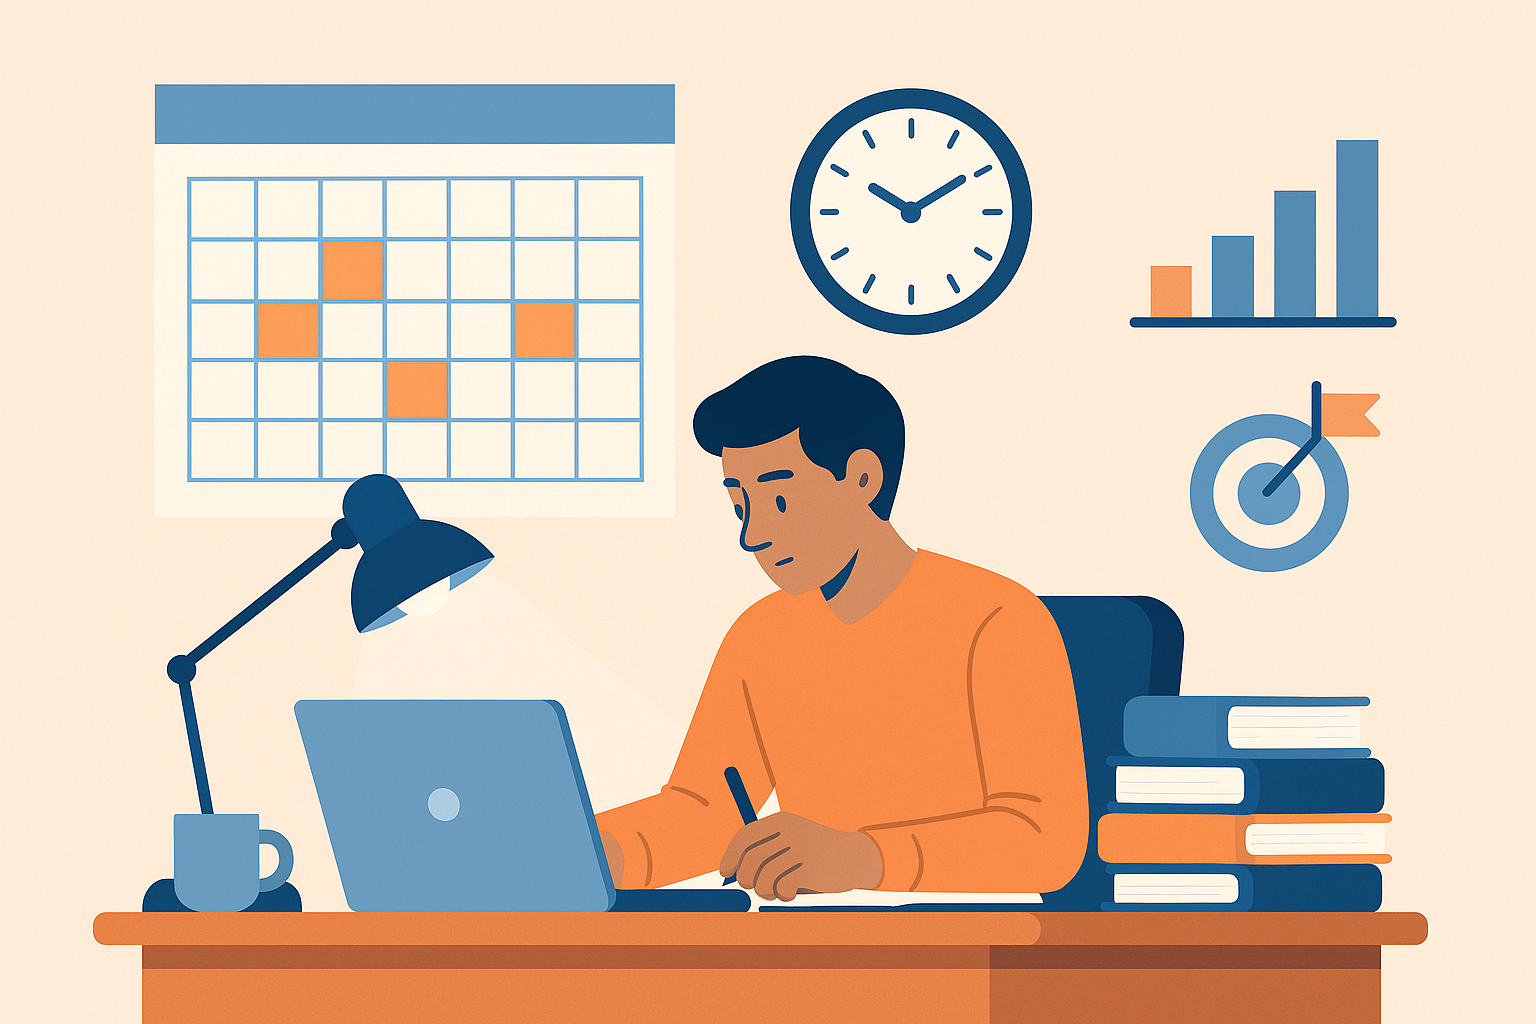
\includegraphics[width=0.5\linewidth]{Images/dedicacao.png}    
\end{center}
\vspace{0.5cm}



\gxatencao{A única maneira de se acabar uma tese é com dedicação.}


Dedicar-se significa reservar horas para seu trabalho de tese. A tese não pode ficar relegada às horas livres, pois essas tendem a sumir rapidamente. 


Dedicar-se significa se esforçar para obter informações, descobrir que informações são necessárias e manter um ritmo de trabalho constante no início e crescente do meio para o final. 


É importante estar preparado para dedicação exclusiva nos dias finais que antecedem a entrega da tese e lembrar de reservar alguns dias para fazer as correções solicitadas pela banca.


A melhor maneira de se dedicar é ter um plano de horários e obedecê-lo, planejar a tese como se fosse um dia de trabalho e cumprir o planejamento. Devo dizer que nunca vi alguém fazer isso, pois as necessidades do dia a dia acabam se encaixando com a flexibilidade dos horários de estudo e “bagunçando o coreto”. Mas aqui vão algumas dicas para organizar sua dedicação:

\begin{outline}
\1	Carga Horária


\2	Determine uma carga horária mínima por dia, por semana e por mês. Tente cumprir todas as cargas horárias. Nunca deixe a carga mínima do mês atrasar.


\1	Metas Específicas


\2	Defina metas específicas, principalmente quando relacionadas à parte do texto da tese e parte do software. Dê um prazo para essas metas. Tenha metas objetivas para cada final de período letivo.


\1	Horário de Trabalho


\2	Defina um horário de trabalho preferido. Você pode ser do tipo madrugador ou noturno. Aproveite a flexibilidade para trabalhar na hora que produz mais. 


\3	Ao longo do tempo, apesar de madrugador, passei a considerar que é mais produtivo que a tese seja seu primeiro trabalho do dia, de modo que você não esteja nem cansado, nem influenciado por outros problemas. Assim, recomendo a meus alunos que têm atividades paralelas acordar pelo menos uma hora mais cedo todo dia para trabalhar na tese.


\1	Aos que dormem tarde, garanto que com o tempo passarão a dormir mais cedo.
\end{outline}

\section{Avaliando Seu Trabalho}


Uma maneira de saber como seu trabalho está andando é avaliá-lo periodicamente. Todo dia se pergunte: eu fiz algo para atingir meu objetivo?


Duas perguntas são importantes em relação aos seus objetivos de tese:

\begin{outline}
\1	O que você escreveu?


\2	Tem relação ao seu trabalho escrevendo capítulos da tese, programas, especificações e artigos em revista. 


\2	Responda à pergunta: em quantos trabalhos desse tipo eu coloquei algum esforço hoje e produzi algum resultado palpável?


\1	Com quem você colaborou?


\2	Tem relação aos tipos de colaborações que você fez nesse dia, semana ou mês. Formas de colaboração possível são:


\3	Fiz algo para meu orientador?


\3	Fiz algo para um colega?


\3	Pedi algo para um colega? 


\3	Dividi algo com um colega?
\end{outline}

\section{Objetivos S.M.A.R.T.}


Um método interessante de criar objetivos em seu trabalho, ou em sua vida em geral, é lembrar do acrônimo S.M.A.R.T. Segundo essa teoria, um objetivo deve ser:

\begin{outline}
\1	S – eSpecífico (Specific)


\2	O objetivo deve ser específico e não generalizado. Ou seja, deve ser algo que pode ser claramente atingido. Um bom exemplo é “entrar em uma academia e me exercitar 3 vezes por semana” e não “malhar”. 


\1	M – Mensurável (Measurable)


\2	Deve ser possível avaliar que ele foi atingido. O exemplo típico é ótimo: “perder 5 quilos”.


\1	A – Atingível (Attainable)


\2	O objetivo tem que ser alcançável. Você tem que se propor a realizá-lo e tem que compreender suas dificuldades.


\1	R – Realista (Realistic)


\2	O objetivo tem que ser realista. Não adianta querer perder 50 quilos em uma semana. 


\1	T – limitado no Tempo (Time Bound)


\2	Você tem que dar um prazo para o objetivo acontecer. Por exemplo “Perder 5 quilos em 3 meses”.


\2	Alguns autores consideram T para “Tangível”, no sentido de ser algo que possa ser avaliado de acordo com os 5 sentidos (tato, paladar, visão, audição e olfato). 
\end{outline}

Relacionados à tese, bons objetivos podem ser:

\begin{itemize}
	\item	Escrever um capítulo de revisão bibliográfica de 15 páginas em um mês.
	
	
	\item	Escrever um artigo descrevendo a experiência realizada até dia 30 de setembro.
	
\end{itemize}


Devemos lembrar que os prazos que recebemos da instituição e de congressos e revistas são ótimos mecanismos para determinar nossos limites no tempo.



\section{Técnicas de Estudo e Trabalho}


Existem muitas maneiras de trabalhar e estudar, principalmente na frente do computador. Quero chamar atenção a uma técnica e uma teoria que são muito difundidas, mas que são opostas, respectivamente, Pomodoro, Flow (ou Fluxo).


Fluxo é uma teoria proposta por Mihaly Csikszenbtmihalyi que diz que existe um estado de alta concentração onde entramos em fluxo. O fluxo é um estado da mente onde estamos altamente focados no trabalho, não sentimos o tempo passar. Para alcançar o fluxo cada pessoa precisa de um certo tempo, que pode chegar a 30 minutos. Porém, se perdemos a concentração, saímos imediatamente do estado de fluxo e voltamos a precisar do mesmo tempo para entrar de novo nele. 


Seguindo esse caminho, é importante reservar momentos mais longos e com nenhuma interrupção. Se desligar do celular e das redes sociais é essencial para atingir o Fluxo.


Pomodoro é uma prática de estudo onde treinamos o cérebro para funcionar focado em curtos períodos. Tradicionalmente se usa 25 de trabalho por 5 de descanso por ciclo, mais 15 a 20 minutos de descanso depois de 3 ciclos. A principal parte dessa técnica é gerenciar as distrações.


Claramente a técnica Pomodoro interrompe o estado de fluxo. Não está claro qual escolher, talvez algumas tarefas sejam adequadas a procurar o fluxo e outras a técnica de Pomodoro. Pessoalmente eu reconheço minha capacidade de entrar em estado de fluxo quando faço tarefas como escrever algo ou programar, conseguindo grande concentração. Confesso que as vezes, ao sair do fluxo, tenho até dificuldade de entender de novo o código que escrevi. Já a técnica Pomodoro não funciona bem comigo, que tenho tendência a procurar desculpas para exceder o tempo de descanso, me envolvendo com outras atividades.


Sugiro aos leitores que se aprofundem mais nas duas técnicas, façam experimentos consigo mesmos e escolham a que mais se adapta ao seu estilo.


\section{Ambiente de Estudo}


Uma das coisas mais importantes é ter um ambiente de estudo onde você se sinta bem. Alguns preferem o silêncio, outros necessitam de música, cada um tem um gosto pessoal. Aqui vão algumas dicas: 

\begin{itemize}
\item	Tenha um computador próprio e exclusivo. 


\item	Lembre-se: você é um aluno de Computação, o mínimo que pode ter é um computador próprio.


\item	Isso também é uma defesa, já que você não quer que outros destruam sem intenção o seu trabalho.


\item	Tenha um ambiente de estudo em casa e um na faculdade. 


\item	Cultive esses ambientes, retirando dele tudo que pode atrapalhar sua concentração e usando-os prioritariamente. 


\item	Em cada início de período dê uma “arrumada” no seu computador, evitando assim problemas graves no meio do período. 


\item	Evite estudar em uma posição que leve ao sono. 


\item	Tenha uma estante reservada para o material de estudo. 


\item	Mantenha seus artigos organizados. Encaderne-os ou coloque-os em fichários, ou em diretórios organizados. Eu uso o software Calibre para todos meus PDFs, por exemplo.
\end{itemize}

\section{O Método do Tadeu}


Um dos alunos mais organizados que tive foi o Tadeu Classe. Ele me mandou esse relato sobre como se organiza.

\begin{quote}
Desde que comecei meu doutorado constantemente vinha percebendo que precisava organizar melhor as minhas tarefas. Sou um doutorando que não faz somente a sua pesquisa, pois preciso me manter na cidade onde vivo, e tenho outras atividades, como treinos esportivos, lecionar em instituições de ensino superior e trabalhar como analista de sistemas.

\begin{figure}[hbt]
	\centering
	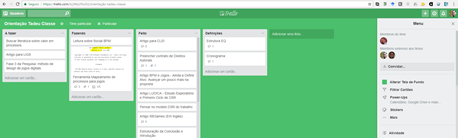
\includegraphics[width=0.7\linewidth]{Images/Trello}
	\caption{Imagem do Trello, software que o Tadeu usou durante sua tese. Fonte: imagem fornecida por Tadeu Classe}
	\label{fig:trello}
\end{figure}

Devido a isso, a minha desorganização vinha tomando conta, e não conseguia desempenhar nenhumas das atividades que realizava com qualidade. Um dos meus orientadores, a Profª. D.Sc. Renata Araujo da UNIRIO, sempre sugeriu desde o início dos meus estudos, que eu tentasse me organizar usando o programa Trello (https://trello.com/), que é um quadro virtual de atividades, onde você consegue organizar e grupos e ir colocando lembretes para a realização das atividades, porém, pessoalmente não gostei muito de usar a ferramenta. Pois mesmo organizando as tarefas, e o que eu precisava fazer, eu não lembrava de acessá-la e atualizá-la.

\begin{figure}[hbt]
	\centering
	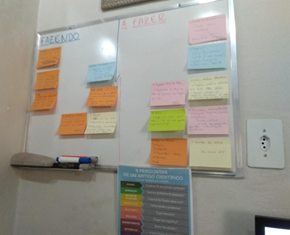
\includegraphics[width=0.7\linewidth]{Images/quadroorganizacao}
	\caption{Quadro de organização de Tadeu Class. Fonte: imagem fornecida por Tadeu Classe.}
	\label{fig:quadroorganizacao}
\end{figure}

Entretanto, me baseando no Trello e para que eu conseguisse organizar melhor os meus afazeres durando meu dia a dia como doutorando, analista de sistemas e professor, decidir colocar em meu escritório de trabalho um quadro branco. Neste quadro eu fiz a sua divisão em duas áreas (“A FAZER” e “FAZENDO”) no qual eu anexo “post-its” com as tarefas que eu preciso realizar [Figura 2], trocando entre os lados as prioridades, sendo que as tarefas que forem sendo realizadas, jogo o post-it no lixo. Meus post-its são coloridos, e cada cor indica o grau de urgência da atividade a ser realizada, por exemplo: laranja: URGÊNCIA, azul: PRECISAM SER FEITOS, rosa: FAZER ASSIM QUE SOBRAR UM TEMPO, amarelo: SEM URGÊNCIA, e verde: UM DIA EU FAÇO.

Desta maneira consegui ter um quadro de tarefas onde consigo organizar tudo o que precisa ser feito em meu dia a dia, com a vantagem de que o mesmo está sempre na minha frente fazendo com que eu sempre esteja olhando para ele. Minha produtividade melhorou muito desde então, e ele me auxiliou a entregar todas as demandas nos prazos corretos.

\end{quote}

\chapter{O Ótimo é Inimigo do Bom}

Se eu tivesse que resumir tudo em uma frase, escolheria 

\gxatencao{O ótimo é inimigo do bom.}


Vamos ver três objetivos durante o curso de pós-graduação:
\begin{itemize}
\item	Você tem que acabar a sua tese. 
\item	Acabar a tese é a coisa mais importante. 
\item	Nada é mais importante que acabar a tese.
\end{itemize}

Está claro? 
A tese é o mais importante!

Para que você possa acabar sua tese, ela tem que estar bem delimitada. Isso não precisa ser feito no início de tudo, mas pelo menos seis meses antes do seu prazo terminar, a tese tem que estar totalmente delimitada. 

Uma tese também não é a palavra final sobre o assunto. É muito pouco provável que você tenha um resultado em sua tese que mude a história da ciência ou o dia a dia das pessoas. 

Sua tese é uma contribuição ao conjunto de trabalhos existentes. Se você acha que sua tese mudará tudo, é bom ter uma conversa séria com seu orientador. 

Quando digo séria, digo uma conversa em que você vai extremamente preparado para provar sua tese ou a possibilidade dela e que levará argumentos e contra-argumentos que apoiem sua previsão. Para falar a verdade, é importante fazer isso qualquer que seja sua tese.

É importante cortar. Sempre queremos escrever mais do que devemos, queremos estudar um pouco mais, queremos entender um pouco melhor aquele detalhe. Porém, o que é realmente importante? Acabar a tese. 

Se a tese só crescer, ela nunca terá fim. Cortando, geramos o foco que permitirá que a tese chegue ao seu bom termo.
Você não precisa ser inteligente para acabar a tese. Precisa ser dedicado e trabalhar muito. Porém, sempre que tomar uma decisão lembre-se dessas regras simples, sugeridas por orientadores e orientados:
\begin{itemize}
    \item A tese tem que acabar. 
    \item O ótimo é inimigo do bom.
    \item Você é humano.
   \item 	Apenas com trabalho se alcançam resultados.
\item	Entre um conjunto de soluções, a mais simples deve ser a primeira a ser tentada.
\item	Quem não se comunica se trumbica
\end{itemize}
	

A experiência diz que os alunos quebram todas essas regras em vários momentos do processo de construção da tese. Eles querem fazer coisas demais, querem ser perfeitos demais, assumem compromissos demais, esperam resultados de graça e tentam soluções complicadas antes de tentar as fáceis. Não quebrando essas seis regras, você facilitará muito o seu trabalho e o do seu orientador.

Também é importante limitar o número de assuntos a serem estudados profundamente. O número ideal é um, mas dois é um número possível. Tentar tratar profundamente de três assuntos está definitivamente fora de questão. Se sua tese é multidisciplinar, escolha assuntos principais e trate os outros como ferramentas ou área de referência.

Para sua tese acabar, você ou seu orientador têm que tomar uma decisão importante: é o fim. Geralmente, em uma reunião se combinam todos os pontos a serem costurados, terminados e abandonados para a tese terminar. A partir desse ponto, o orientador espera apenas verificar o seu texto e resultados, mas não ter nenhuma novidade no processo. Alcançar esse momento é um sinal importante de que você irá defender sua tese logo.

\begin{itemize}
    \item Escreva uma sentença de até 25 palavras sobre o tema da sua tese.
    \item Não misture mais de 2 áreas de pesquisa.
    \item Encontre primeiro o problema, depois a solução.
\end{itemize}

\chapter{Publicando}

\begin{center}

\includegraphics[width=0.5\linewidth]{Images/publicando.png}    
\end{center}
\vspace{0.5cm}


Só existe uma maneira verdadeiramente honesta de avaliar um trabalho científico: submetê-lo a revisão de seus pares. 
Por isso existe uma banca de mestrado e doutorado. Por isso cada vez mais é importante publicar seus resultados.

Na forma atual que alunos, professores e programas de pós-graduação são avaliados é impossível imaginar uma tese onde não houve uma publicação.
A política correta de um orientador deve ser não permitir a defesa de uma tese que não tenha nenhum artigo publicado. Para isso dou dois motivos: se nenhum trabalho foi apresentado para a publicação, então o aluno não demonstrou interesse, se nenhum trabalho foi aceito, a tese não demonstrou capacidade.

Publicar é responsabilidade do aluno. Cabe ao orientador auxiliá-lo nessa tarefa. Claro que, dependendo da capacidade do orientador na área, ele pode ser a força motriz do artigo. Porém, é importante que o aluno tenha a experiência de conduzir a parte principal do trabalho de publicação.

Uma tese de doutorado tem uma obrigação ainda maior: publicar artigos em revista.

Publique sempre. Antes de acabar a tese, depois de acabar a tese. A única maneira de seu trabalho ficar conhecido e você ser reconhecido é por meio de publicações. Aceite ligeiros atrasos em sua tese (que não interfiram com seu prazo) se for para publicar. Publicar dará pontos em concursos públicos para professor e tornará você conhecido na comunidade.

Ao publicar, não esqueça que os autores são, pelo menos, você e seu orientador. Geralmente o aluno vem em primeiro lugar, mas algumas vezes, principalmente quando a ideia principal vem do orientador, o nome dele vem em primeiro. Publicar sem o nome do orientador é um dos maiores pecados que um aluno pode fazer contra a relação aluno/orientador na área da Computação.

A questão da publicação está se tornando cada vez mais séria no Brasil. Tanto a CAPES quanto as universidades estão avaliando seus pesquisadores principalmente em função da quantidade e qualidade das publicações.

 \needspace{5\baselineskip}\section{A Pressão para Publicar Frequentemente}

Devido às metodologias de avaliação a que estão submetidos os diversos programas de pós-graduação, publicar se tornou uma atividade imperativa ao longo de dissertações de mestrado e teses de doutorado.

Normalmente são feitas as seguintes avaliações que consideram as publicações:

\begin{itemize}
  \item Os professores são avaliados dentro de seus programas de pós-graduação, para poder orientar
  \item Os professores são avaliados para promoções
  \item Os professores são avaliados quando fazem pedidos de bolsa ou projetos
  \item Os programas são avaliados pela Capes e pelo CNPq
  \item As universidades são avaliadas pelo MEC, por organismos nacionais e internacionais 
\end{itemize}

 \needspace{5\baselineskip}\section{As Regras da Publicação}

As regras da publicação são:
\begin{enumerate}
    \item Escrever sempre;
    \item Relacione como autores todos os envolvidos;
    \item Sempre envolva seu orientador, e
    \item Escute os revisores.
\end{enumerate}

Tudo que você fizer no mestrado deve levar em conta a possibilidade de uma publicação. Se não permite uma publicação é porque provavelmente não há contribuição.

 \needspace{5\baselineskip}\section{Autoria}

Na Computação é praxe que os artigos sejam feitos com a colaboração direta dos orientadores e alunos.
Em outras áreas isso pode não ser verdade, e os textos podem ter um autor só. Na Medicina, por outro lado, é comum artigos com muitos autores, e existem até regras específicas para colocar uma pessoa como autor ou não\furl{https://www.icmje.org/recommendations/browse/roles-and-responsibilities/defining-the-role-of-authors-and-contributors.html}.


O comportamento esperado é avisar o orientador do artigo desde o início e manter ele dentro do \textit{loop}. Além disso, nunca deixe de apresentar o artigo ao orientador antes de submetê-lo a um congresso ou revista. Só retirar o nome se o orientador pedir.  
Um orientador espera que você trabalhe com ele, e não que saia fazendo trabalhos isolados com outras pessoas. Ele também evitará que você cometa erros grosseiros por inexperiência. 

É melhor errar por incluir algum autor que não merecia estar citado do que excluir um que merecia. 
Não se esqueça de enviar o artigo a todos os autores, pedir sua colaboração e aceitação. 
Não coloque pessoas como autoras sem avisá-las.
Cabe a quem não se interessar solicitar a retirada do seu nome do artigo, e a quem se interessar, participar ativamente.

Sempre se pergunte: esse texto seria produzido, da forma como está, caso a pessoa específica não tivesse dado sua colaboração? 

\subsection{Ordem de autores}

A questão da ordem de autores é normalmente resolvida colocando em ordem decrescente de manipulação do texto. Normalmente, o autor principal é aquele que contribuiu mais para as partes mais importantes do texto. Os orientadores costumam ficar no final.

 \needspace{5\baselineskip}\section{Escolhendo onde publicar}

Para publicar são usados os seguintes critérios na escolha da revista ou congresso:
\begin{itemize}
    \item A adequação do tema ao veículo;
    \item A comunidade a que pertence o pesquisador, que pode se interessar no artigo e como o veículo a atende;
    \item O impacto do veículo na área, seja ela específica ou geral, já que algumas revistas de baixo impacto em geral tem alto impacto em uma área específica, por exemplo, porque essa área tem menos pesquisadores;
    \item A taxa média de aceitação;
    \item O estilo de artigos da revista, já que alguns veículos usam linguagens mais formais, ou mais matemáticas, e outros são mais informais, mesmo que ainda acadêmicos;
    \item A linguagem do veículo;
    \item A velocidade do processo de revisão e publicação, e
    \item O custo de publicação ou apresentação em congresso.
\end{itemize}


Muitas universidades têm acesso a sistemas que permitem verificar o impacto das publicações, como o \textit{Web of Science}. Além disso, quase todas as áreas já conseguiram organizar seu ``Qualis'', uma lista mantida pela CAPES classificada das publicações que tem como objetivo indicar sua qualidade. Essa lista, porém, tem falhas e foi anunciado em 2025 que não será mais mantida.

\gxatencao{O primeiro alvo de suas publicações deve ser os mesmos congressos e revistas que você usa na sua bibliografia.}

\subsubsection{Revistas e congressos predatórios}

Ao buscar onde publicar os resultados de sua pesquisa, é imprescindível estar atento às chamadas \textbf{publicações e eventos predatórios}.
Esse termo refere-se a revistas científicas e congressos que se aproveitam da pressão por publicações acadêmicas para explorar autores, muitas vezes oferecendo visibilidade em troca de pagamento, sem garantir os padrões mínimos de revisão por pares ou curadoria científica.

 Essas revistas e eventos costumam aceitar artigos com critérios mínimos (ou inexistentes) de avaliação de qualidade, desde que o autor pague uma taxa de publicação. 
 É comum que enviem convites genéricos por e-mail, muitas vezes com elogios ao seu ``excelente trabalho'', mesmo sem citar um título específico. 
 Algumas chegam a informar que seu artigo já foi ``pré-selecionado'' e que a publicação ocorrerá rapidamente, mediante o pagamento de uma taxa, geralmente com valores entre 50 e 500 dólares.

\textbf{Sinais de alerta incluem:}
\begin{itemize}
  \item Ausência de revisão por pares ou um processo extremamente rápido de aceitação;
  \item Convites genéricos para submissão enviados por e-mail em massa;
  \item Convites repetidos para diferentes trabalhos em Congresso feitos pela mesma editora;
  \item Convites para revistas com nomes muito genéricos ou para revistas com nomes que não têm relação com seu artigo;
  \item Promessa de publicação garantida ou prazos de resposta muito curtos;
  \item Taxas elevadas sem justificativa, cobradas logo na submissão;
  \item Títulos enganosos que imitam revistas renomadas;
  \item Sites com informações vagas sobre o corpo editorial, indexadores ou política de ética.
\end{itemize}

Eventos predatórios também merecem atenção. Alguns congressos internacionais, muitas vezes organizados por empresas comerciais, agregam dezenas ou centenas de trilhas temáticas desconexas, com nomes genéricos como \textit{``World Congress on Advances in Science, Engineering and Technology''}. 
Esses eventos geralmente aceitam qualquer resumo e cobram taxas de inscrição elevadas, oferecendo pouco retorno acadêmico. Frequentemente, os anais nem sequer são indexados em bases reconhecidas.

\textbf{Como se proteger:}
\begin{itemize}
  \item Consulte seu orientador ou colegas mais experientes.
  \item Verifique se a revista está indexada em bases respeitadas como \textit{Scopus}, \textit{Web of Science}, ou tem fator de impacto no \textit{Journal Citation Reports}.
  \item Consulte o site do \textit{Committee on Publication Ethics} (COPE)\footnote{\url{https://publicationethics.org}} e a lista de revistas confiáveis mantida por universidades.
  \item Verifique se a editora é associada a organizações legítimas como o \textit{Directory of Open Access Journals} (DOAJ).
  \item Desconfie de congressos com escopo excessivamente amplo e sem revisão técnica clara.
\end{itemize}

O conceito de publicação predatória foi inicialmente formalizado por Jeffrey Beall, bibliotecário da Universidade do Colorado, que manteve por anos uma lista pública de editoras e periódicos suspeitos. Apesar da lista original ter sido descontinuada, versões arquivadas e alternativas ainda são úteis como ponto de partida.

Lembre-se que publicar em revistas ou congressos predatórios pode comprometer sua credibilidade acadêmica. 
Uma publicação nesse tipo de veículo não apenas não é valorizada, como pode prejudicar sua avaliação em seleções de bolsas, concursos ou progressões acadêmicas.


 \needspace{5\baselineskip}\section{Plágio e Citações}

Basicamente, plagiar significa apresentar como seu trabalho que foi feito e já publicado por outro. 
No mundo acadêmico, o plágio é considerado uma desonestidade séria e é punido de várias formas, formais e informais, como a exclusão de um curso, a reprovação de um trabalho ou em uma cadeira, a demissão de professores e até mesmo, em alguns casos, sendo levado à justiça comum.

Isso significa que todo texto para o qual assumimos a autoria deve ser original, sob o risco de incorrer em plágio. 
Obviamente, não é possível fazer trabalho científico sem se utilizar de ideias e textos de outros autores como ponto de partida e apoio, logo existem regras claras de como realizar \textbf{citações e referências}, isto é, como descrever o trabalho de outro de forma que fique clara a atribuição de autoria.

No Brasil existe uma norma de citação mantida pela ABNT e muitas universidades mantêm versões próprias, inspiradas na ABNT. Nessas normas se descrevem, de forma bastante detalhada, as várias maneiras de se declarar uma citação. Nem sempre, porém, fica claro o que é uma citação.

Existem duas formas de citação: a citação direta e a citação indireta. 

Na citação direta copiamos diretamente o texto do autor e, por causa disso, devemos marcar de forma clara que estamos fazendo essa cópia. Segundo a norma ABNT isso é feito pelo uso de aspas, quando a citação tem até 3 linhas, ou usando um parágrafo com recuo de 4 cm da margem esquerda]\citep{abnt10520_2023}.

\begin{quote}
``citações indiretas (ou livres) são a reprodução de algumas idéias, sem que haja transcrição das palavras do autor consultado. Apesar de ser livre, deve ser fiel ao sentido do texto original. Não necessita de aspas.'' \citep{abnt10520_2023}
\end{quote}

Nos dois parágrafos acima fizemos uma citação indireta ao descrever a direta e uma citação direta ao descrever uma indireta. 

 \needspace{5\baselineskip}\section{Como trabalhar um artigo em grupo}

Apesar de facilitar o trabalho, escrever um artigo em grupo, principalmente se feito remotamente, cada um em um local diferente, não é uma tarefa fácil. O trabalho de um pode destruir o trabalho de outro, estilos podem ficar misturados, etc.

Algumas recomendações:

\begin{itemize}
  \item É possível fazer grande parte do trabalho textual em um editor on-line. Hoje é minha opção preferida, usando o \textit{Overleaf}, um ambiente para escrever em \LaTeX. As opções são: Google Docs e a versão nuvem do Microsoft Word. 
  \item Overleaf é uma boa opção para o mundo \LaTeX, porém para compartilhar entre muitas pessoas, deve ser pago. Eu pago, e costumo abrir projetos para meus alunos poderem fazer sua tese e artigos. Nem todas revistas aceitam artigos em PDF ou em formato \LaTeX.
  \item A versão final deve provavelmente ser feita em LaTeX ou Word, devido a capacidade de formatação. Para isso use serviços com Google Drive e OneDrive, compartilhando pastas. Algumas revistas aceitam vários formatos, outras apenas um.
  \item Use um sistema de controle de versão, como git e GitHub, ou, se não usar o controle de versão, use nomes para controlá-la. O nome do arquivo deve ser algo do tipo \texttt{Nome do artigo – parte – versão – autor que fez a versão.docx}.\\
  Exemplo: \texttt{theboss texto v10 xexeo.docx}. 
\end{itemize}

\subsection{Organização e versionamento}

Mantenha a última versão do artigo na raiz do seu diretório, junto com a template original da revista ou congresso e o call for papers.

Mantenha diretórios separados que indicam o que está nele, como em:
\begin{itemize}
  \item \textbf{Versões antigas}
  \item \textbf{Subsídios} (contendo cópias de todas as referências usadas e até mesmo algumas não usadas, como referência de escrita)
  \item \textbf{Dados} (todos os dados usados para escrever o artigo, na medida do razoável pelo consumo de espaço)
  \item \textbf{Programas} (todos os programas usados para processar os dados)
  \item \textbf{Resultados} (todos os resultados obtidos)
  \item \textbf{Software} (links ou software usado no processamento, na medida do razoável para utilização)
\end{itemize}

Além disso: 

\begin{itemize}
  \item Mantenha a revisão ligada no Word e no Overleaf.
  \item Sempre que mudanças forem feitas, faça uma nova versão do artigo, criando uma versão e passando as velhas para o diretório de versões antigas, ou fazendo commit.
  \item Possivelmente quebre o artigo em partes.
  \item Mantenha o formato da conferência o mais cedo possível, para ter ideia de tamanho.
  \item Se comunique via meios eletrônicos para registrar as comunicações. 
  \item Em certo ponto, congele o crescimento do artigo, para se preparar apenas para revisões e correções. 
  \item Ao congelar, peça para todos os autores fazerem sua última revisão. 
  \item Tente dar ao menos 24 horas para isso.
  \item Marque uma reunião final para fechar o arquivo e para que todos possam submeter conjuntamente ou concordar que um será responsável pela submissão.
\end{itemize}

Não se esqueça que existem softwares muito poderosos de controle de referência que serão essenciais à sua tese. Em especial, o uso do bib\LaTeX e bib\TeX no \LaTeX, com apoio do JabRef e o uso do controle de referências com Zotero instalado no Word são meus preferidos.


 \needspace{5\baselineskip}\section{Submissão}

Nada revela mais sobre a maturidade de uma pesquisa do que apertar o botão ``submit''. O processo costuma ser:

\begin{enumerate}
\item Definição do artigo;
\item Início da escrita ou de uma versão inicial de trabalho;
  \item Escolha  do periódico ou conferência, analisando
        fator de impacto, escopo temático e tempo de resposta;
    \item Determinação de como deve ser um artigo para o meio escolhido;
    \item Escrita do artigo de acordo com o estilo do meio;
  \item Checklist de integridade: ORCID, conflitos de interesse, aprovações do comitê de ética, declaração de dados abertos;
  \item Ajuste fino de formatação, cuidando do template, formatos de referência, figuras em alta resolução;
  \item Submissão; 
  \item Acompanhamento da revisão; \label{passo:acompanhar}
  \item Se irritar com as respostas, mesmo quando positivas em geral;
  \item Realização os acertos necessários; 
  \item Envio a versão (supostamente) final;
  \item Espera da publicação, e
  \item Atualização do Lattes e divulgação entre os pares.
\end{enumerate}

\gxatencao{Nunca submeta um mesmo artigo para dois lugares simultaneamente.}


 \needspace{5\baselineskip}
 \section{Revisão por pares}

Após uma primeira vista do Editor, que pode devolver, por achar que o artigo não cabe na revista, ou recusa imediata, normalmente a revisão é feita por dois ou mais revisores, no formato ``duplamente cego''.  Isso significa que os revisores não sabem quem são os autores e vice-versa. 

O processo, apesar de buscar garantir a qualidade das publicações, é muito cansativo para os editores e revisores e traumático para os revisados. 

É comum que, ao ler uma revisão, os autores encontrem erros, falta de respeito com o trabalho e pedidos absurdos, como refazer todos os experimentos, considerar uma teoria completamente diferente ou genérica demais. 
Já recebi revisões que simplesmente diziam que um bom resultado devia ser mentira e recusavam o artigo com base nessa hipótese, e revisões de outro artigo, como se fossem o meu. Em congressos, onde o processo é massivo e rápido, os erros são mais comuns.

As respostas normalmente se enquadram em: aceitação, aceitação com revisões menores (\textit{minor revision}), o que é praticamente a aceitação, aceitação com revisões maiores (\textit{major revision}), o que pode variar entre uma recusa educada ou uma aceitação com grandes exigências, o que até mesmo pode levar a desistência dos autores de seguir o processo com aquela revista, recusa pelo resultado da revisão, recusa pelo editor (por não ser do tema da revista ou não atingir parâmetros mínimos, até de formatação), ou ainda devolução pelo editor por não encontrar revisores ou achar que o artigo não é do tema da revista.

Mesmo aceitos, muitos artigos passam ainda por um processo de publicação que inclui revisões simples, provas de impressão ou outros pedidos de revisão.

Ao receber o parecer, e este não foi uma recusa, siga esta sequência de sobrevivência:

\begin{enumerate}
  \item Leia tudo uma primeira vez.  
  \item Deixe a raiva decantar por 24 h.  
  \item Construa uma tabela \textit{Pedido do Revisor, Proposta de Resposta}. Considere que alguns pedidos podem não ser realizáveis, e possivelmente representam na prática uma recusa. 
  \item Chame os co-autores para discutir o que será feito, que inclui:
  \begin{itemize}
      \item Fazer as revisões, possivelmente todas,  para a mesma revista, se isso é possível;
      \item Fazer as revisões e enviar para outra revista;
      \item Fazer algumas revisões, e
      \item Variações sobre o tema...
  \end{itemize}
\end{enumerate}

É importante enviar, junto com o novo artigo, uma carta explicando tudo que foi feito, o que foi atendido e contrapondo o que decidiram não fazer. 
A tabela ajuda a escrever a carta. 
Faça isso mesmo que ela não seja obrigatória. 
Essa carta deve ser muito detalhada, apontando e repetindo, se possível, as modificações no texto. 
Por exemplo, você não deve só dizer que trocou a figura 1, mas também mostrar a anterior, a nova, e escrever como as modificações atendem o pedido do revisor.

\gxatencao{Se seu artigo foi recursado, aproveite os comentários e faça uma versão para uma nova revista ou congresso.}


 \needspace{5\baselineskip}\section{A lenda do Revisor 2}

No folclore acadêmico, sempre há um Revisor 2 pronto a criticar seu trabalho de forma errônea ou cruel. Entre os poderes dessa super-vilão estão:
\begin{description}
  \item A Onisciência, pois conhece todos os \emph{state of the art} publicados na semana passada;
  \item A Limitação, pois desconhece outras áreas e tem dificuldade de entender abordagens interdisciplinares;
  \item A Telepatia, pois detecta suposições não escritas e quer ver todas testadas, e 
  \item A Contradição, pois pede mais informações, mas sugere reduzir o artigo.
\end{description}

Para lidar com isso:
\begin{enumerate}
  \item \textbf{Não personalize}, o ataque ao trabalho não é um        ataque à pessoa;
  \item \textbf{Busque a causa raiz} do ataque e como pode ser resolvido;
  \item \textbf{Converta sugestões em ação}, se a amostra é pequena,    inclua análise de poder estatístico; se faltam referências, cite-as;
  \item \textbf{Negocie com dados}, quando discordar,
        explique por que determinada modificação comprometeria o método ou extrapolaria os limites do estudo.
\end{enumerate}

Submissão e revisão compõem um ciclo virtuoso: 
construímos, testamos, corrigimos, reconstruímos.  
E, à medida que enfrentamos cada novo Revisor 2, fica claro que
publicar é menos sobre ser perfeito e mais sobre ser 
\emph{iterativamente melhor}. Muitas vezes, um artigo recusado se torna muito melhor quando as sugestões são seguidas e fazem sucesso em outro lugar.


\chapter{Metodologia Científica}

\begin{center}
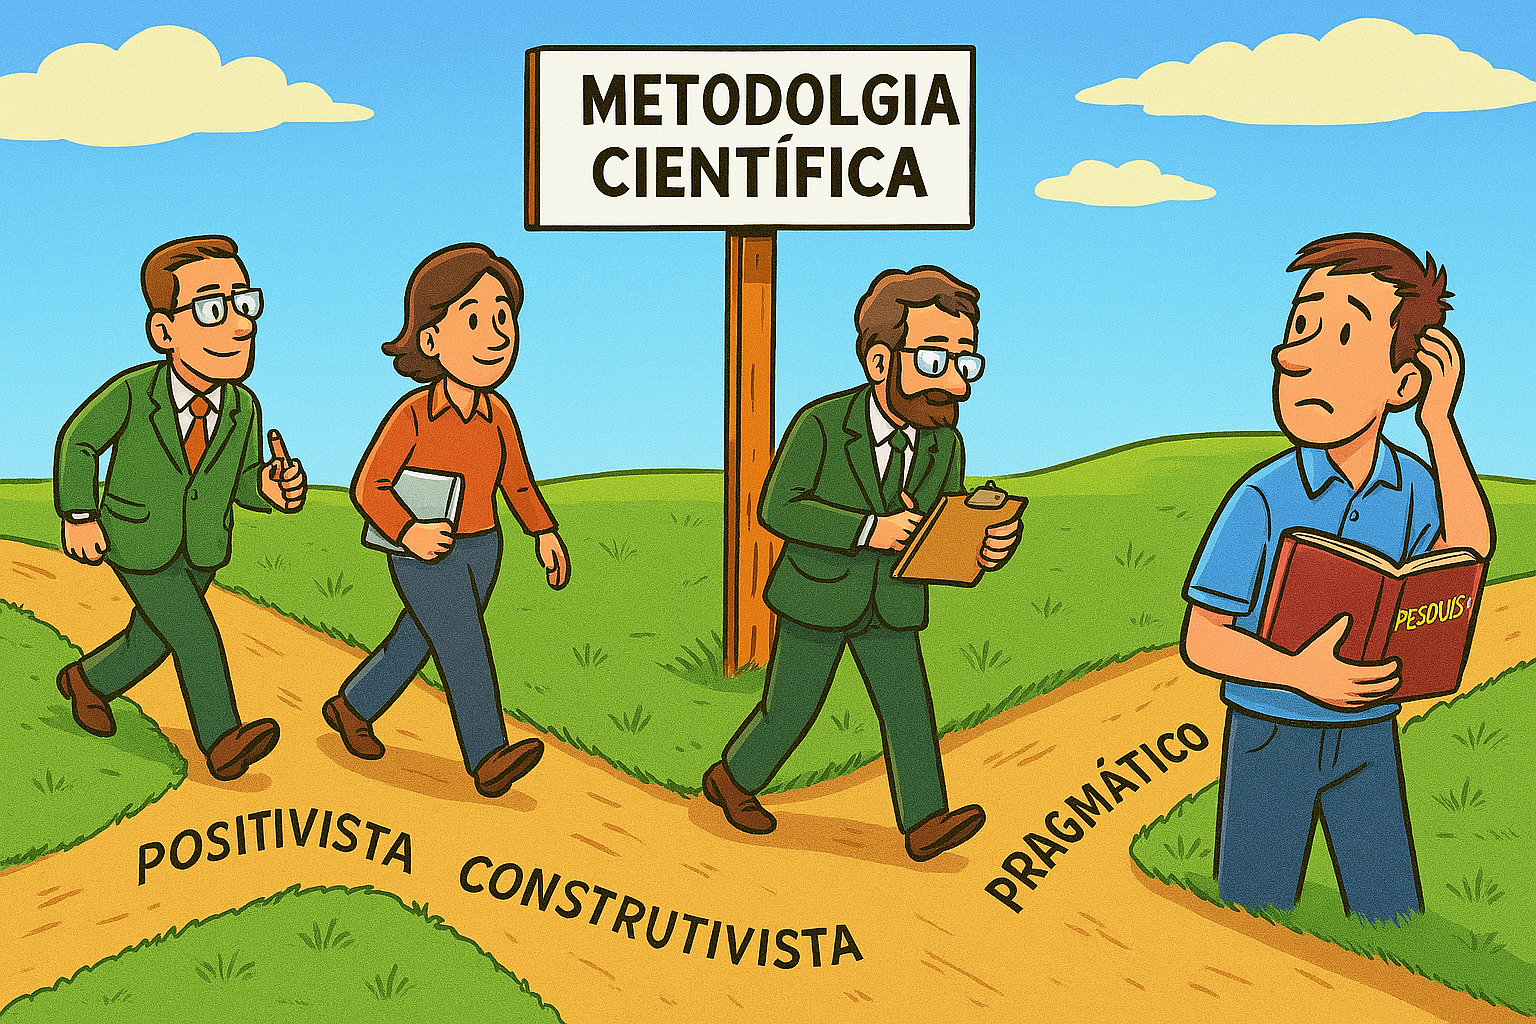
\includegraphics[width=0.5\linewidth]{Images/metodologia.png}    
\end{center}
\vspace{0.5cm}



Não pretendemos, neste capítulo, fazer uma discussão complexa do que é o método científico, mas mostrar algumas noções básicas que devem ser pensadas \textbf{antes} ao começar o trabalho. 

A escolha explícita e consciente do método científico frente a um contexto e questão de pesquisa é complexa e depende de vários fatores. 
Porém, na prática, ela acaba sendo muitas vezes implícita, pois é feita na base da cópia, adaptação e evolução das práticas usadas pelo grupo com que trabalha, que têm grande impacto nessa escolha. 

Uma pesquisa se baseia em uma perspectiva filosófica, ou paradigma filosófico, que muitas vezes é implícita. 
Existem várias perspectivas filosóficas, e \citet{creswell2021projeto} chamam a atenção para quatro: a positivista e pós-positivista, a construtivista, a transformativa e a pragmática. 

Esses quatro paradigmas diferem fundamentalmente em suas concepções de realidade, conhecimento e o papel do pesquisador. O \gxdefine{paradigma positivista} e pós-positivista busca a objetividade, baseando-se em métodos quantitativos para testar hipóteses e estabelecer leis gerais por meio de mensuração e experimentação. Já o \gxdefine{paradigma construtivista} enfatiza a construção social da realidade, valorizando a subjetividade e a interpretação, com forte predileção por métodos qualitativos, como entrevistas e observações. \gxdefine{O paradigma transformativo}, por sua vez, está comprometido com a justiça social e a emancipação de grupos marginalizados; ele frequentemente adota métodos mistos, combinando abordagens quantitativas e qualitativas para dar voz a participantes e provocar mudanças estruturais. Por fim, o paradigma pragmático é orientado pela resolução de problemas e pela utilidade prática do conhecimento, e por isso tende a adotar métodos mistos de forma flexível, escolhendo técnicas com base em sua eficácia para responder às questões de pesquisa~\citet{creswell2021projeto}.

Não cabe a este texto entrar profundamente no tema, mas é possível que seu  grupo de trabalho, mesmo não ``sabendo'', esteja envolvido com um paradigma específico. 
Por exemplo, é comum que pesquisas em Engenharia sigam a perspectiva positivista ou pós-positivista, enquanto as áreas de Humanas têm escolhido muitas vezes o paradigma transformativo.
Principalmente o candidato ao doutorado tem muito a ganhar entendendo qual o paradigma de pesquisa que segue, ou que deveria estar seguindo, e quais métodos e atividades de pesquisa são mais adequados no contexto.

Fica aqui, porém, um aviso: é difícil defender uma tese dentro de um ambiente que adota um paradigma filosófico usando outro paradigma. 

\section{O Método Científico}

Partimos de uma visão do método científico que é bastante geral, apresentada por \citet{Bunge2002}, que é uma visão epistemológica da investigação científica como uma sequência de atividades~\citep[p. 39-40]{Bunge2002}\footnote{Tradução livre do autor}:
\begin{quote}
\begin{enumerate}
    \item Descobrimento do Problema ou lacuna em um conjunto de conhecimentos. Se o problema não está enunciado com clareza, se passa à etapa seguinte, se não, à subsequente;
    \item Descrição precisa do problema, se possível em termos matemáticos, mas não necessariamente quantitativos, ou uma nova descrição de um velho problema a luz de novos conhecimentos 
    \item Busca de conhecimentos ou instrumentos relevantes ao problema (por exemplo, dados empíricos, teorias, aparatos de medida, técnica de cálculo ou de medida). Ou seja, inspeção do conhecido para ver se é possível resolver o problema;
    \item Tentativa de solução do problema com ajuda dos meios identificados. Se essa tentativa falha, passasse à etapa seguinte, se não, à subsequente.
    \item Invenção de novas ideias (hipóteses, teorias ou técnicas) ou a produção de novos dados empíricos que prometam resolver o problema;
    \item Obtenção uma solução, exata ou aproximada, do problema com auxílio do instrumental conceitual ou material disponível;
    \item Por a prova a solução, por exemplo, com ensaios de laboratório ou de campo, e
    \item Correções necessárias nas hipóteses ou técnicas, ou mesmo na formulação do problema original.
\end{enumerate}
\end{quote}

Essa descrição, ilustrada na Figura \ref{fig:bunge}, é o que se chama na Engenharia de Software de um processo Linear ou em Cascata, mas é óbvio que isso é só uma abstração que facilita a descrição a nível epistemológico. A pesquisa científica é um processo de aprendizado constante, e muitas vezes é necessário, após uma etapa, voltar atrás, ou pular à frente, de forma a melhorar a compreensão do problema, das soluções possíveis, corrigir experimentos, etc.

\begin{figure}[hbt]
    \centering
	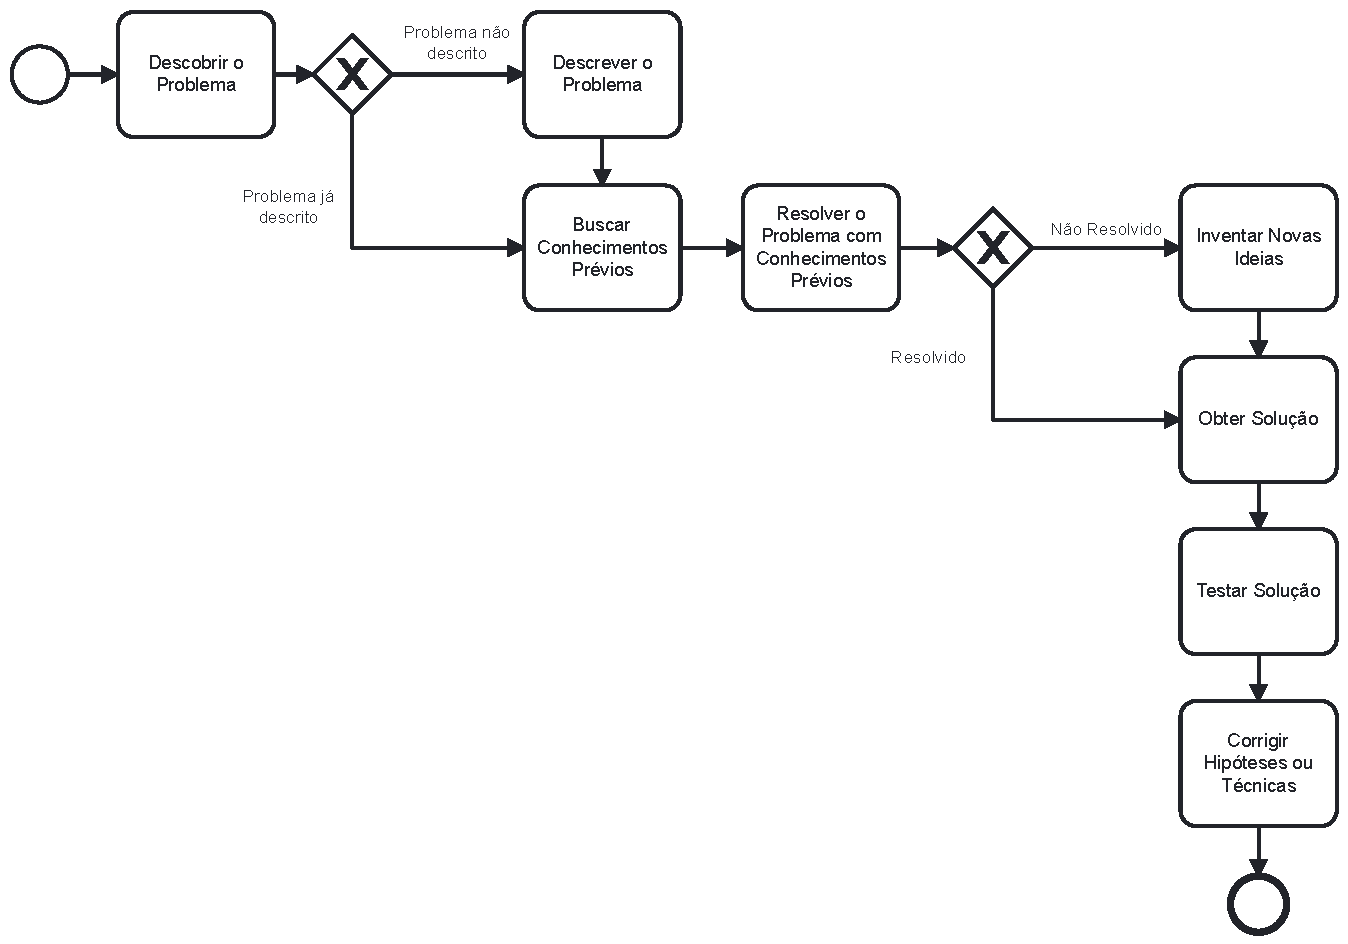
\includegraphics[width=0.7\linewidth]{Images/metodologiabunge.pdf}
    \caption{Metodologia Científica segundo \citet{Bunge2002}, descrita em BPMN~\citep{omg2013bpmn}. Fonte: Do Autor}
    \label{fig:bunge}
\end{figure}

O Mario Bunge ainda diz que para que uma ideia seja considerada científica é necessário, mas não suficiente, que ela seja objetivamente testável com dados empíricos~\citep[p. 37]{Bunge2002}\footnote{Essa sentença segue um dos princípios centrais do realismo científico sistemático e do pós-positivismo crítico caracterizado por Bunge.}.

Ainda mais, \citet[p. 40]{Bunge2002} cita \citet{Kuhn1970}, que diz que a melhor forma de aprender a planejar e resolver problemas científicos não é estudar um manual de metodologia, mas \textbf{estudar e imitar paradigmas ou modelos de investigações que tiveram êxito}. \citet{Kuhn2018}, em seu posfácio de 1969, cita outro autor, Michael Polanyi,  e defende o conhecimento tácito,  dizendo que ele ``é aprendido fazendo ciência, ao invés de adquirindo regras para fazê-la''~\citep[p. 160]{Kuhn2018}\footnote{O que é um sinal de aviso sobre este texto!}. 

Analisando estas falas, podemos concluir que mais do que decorar métodos e segui-los rigidamente, o importante é praticar a ciência e se aproveitar das lições aprendidas.

Escolhendo um método científico muito específico, por exemplo, uma variante da\textit{ Design Science Research}\citep{hevner2004design,Pimentel2019}, o candidato deve estar ciente das questões envolvidas, e ao seguir ou adaptar método, compreender o motivo de suas decisões. 

Essa questão precisa ser discutida, e tratada entre orientador e orientado.

\section{Propor e Comprovar}

Uma tese é uma proposta científica que avança o estado da arte. 
Ou seja, ao escrever sua tese você está se propondo a melhorar alguma coisa. 
Mas não basta apenas a sua opinião de que algo realmente melhorou, ou seja, que sua contribuição é útil: é necessário comprovar essa melhora.

Na abordagem empírica, é necessário construir um experimento ou fazer uma observação. Em uma abordagem teórica, as necessidades podem incluir provar um teorema.

Basicamente existem duas formas de comprovar algo: quantitativamente ou qualitativamente. No primeiro caso, você terá números claros que indicam a melhoria. Por exemplo, após rodar várias vezes dois algoritmos, em diferentes bases de dados, você pode concluir que um é duas vezes mais rápido do que o outro. Já ao comparar duas interfaces em um sistema, você pode fazer perguntas em aberto e fazer, qualitativamente, comparação subjetiva.


Lembre-se do que falou Werner Von Braun:
\gxatencao{Um resultado de um teste vale um milhão de opiniões de especialistas.}

Experimentos se tornam cada vez mais essenciais como forma de comprovação nas teses de STEM e que propõem artefatos. Se no passado a própria proposta era considerada uma contribuição, ou se em alguns lugares isso ainda é aceito, principalmente para níveis de TCC e mestrado, a tendência atual é que um aluno não vá defender um trabalho científico sem algum tipo de tentativa de comprovação científica de sua proposta, mesmo que seja limitada a um contexto específico.

Nesse ponto, é importante lembrar que propostas de artefatos, como softwares dedicados a melhorar algum desempenho humano, dificilmente podem ser comprovadas como melhorias absolutas em todos os casos, já que seus testes são feitos com grupos limitados de pessoas, dentro de contextos específicos. Mesmo sistemas testados com grandes bases de dados estão limitados, em suas conclusões, aos dados usados.

% Não confie cegamente na Internet.  Utilize o senso crítico e analise a importância da referência que está usando. Revistas indexadas são importantes fontes, congressos também. Outra fonte boa de artigos, principalmente para se aprofundar em um tema, são os relatórios técnicos produzidos pelas universidades. 

\section{Termos Importantes}
\begin{itemize}

    \item \textbf{Empírico}: Termo usado para designar conhecimentos ou abordagens baseados em observação direta, experimentação ou análise de dados reais. Na pesquisa científica, métodos empíricos são fundamentais para validar hipóteses, avaliar fenômenos e sustentar conclusões com evidências concretas.

  \item \textbf{Premissa}: Proposição aceita como verdadeira ou ponto de partida lógico sobre o qual se baseia um argumento ou raciocínio. Exemplo: ``Algoritmos de aprendizado de máquina podem ser aplicados à detecção de doenças cardíacas.''

  \item \textbf{Hipótese}: Suposição fundamentada que se pretende testar empiricamente. É uma afirmação passível de verificação que busca explicar um fenômeno ou prever um resultado. Exemplo: ``A aplicação da Transformada Wavelet melhora a acurácia da detecção de arritmias.''

  \item \textbf{Hipótese Nula} (\textit{H\textsubscript{0}}): Formulação contrária à hipótese de pesquisa, utilizada como ponto de comparação estatística. Assume que não há efeito, relação ou diferença significativa. Exemplo: ``A Transformada Wavelet não tem impacto significativo na acurácia da detecção de arritmias.''

  \item \textbf{Tese}: Afirmação central que será defendida ou demonstrada ao longo do trabalho. Pode sintetizar a conclusão antecipada da pesquisa. A tese é uma proposição central que o pesquisador defende ao longo do trabalho. Ela expressa a ideia principal ou conclusão que será sustentada com base em argumentos, dados e evidências. Pode ser resultado da validação de uma hipótese, mas também pode emergir de interpretações teóricas ou reflexões críticas. A tese representa o posicionamento do autor após o processo investigativo.

  \item \textbf{Objetivo}: Intenção geral que orienta a pesquisa; representa o que se busca alcançar de forma ampla. Exemplo: ``Propor uma estratégia eficiente para a classificação de arritmias em sinais de ECG.''

  \item \textbf{Objetivo Específico}: É um desdobramento operacional do objetivo geral da pesquisa. Define, de forma clara, concreta e mensurável, as etapas intermediárias que devem ser alcançadas ao longo do trabalho. Cada objetivo específico deve contribuir diretamente para o cumprimento do objetivo geral, orientando atividades como levantamento bibliográfico, desenvolvimento de métodos, experimentação e análise dos resultados. Eles devem ser redigidos com verbos no infinitivo (como ``analisar'', ``comparar'', ``desenvolver'', ``avaliar'') e evitar ambiguidade ou formulações excessivamente amplas.

  \item \textbf{Meta}: Resultado específico, mensurável e atingível dentro de um prazo determinado. Geralmente associada ao planejamento e execução do projeto. Exemplo: ``Treinar um modelo com acurácia superior a 90\% em um conjunto de validação.''

  \item \textbf{Questão de Pesquisa}: Pergunta central que guia a investigação e delimita o escopo do estudo. Exemplo: ``É possível classificar arritmias em sinais de ECG com alta precisão usando apenas recursos computacionais locais?''
\end{itemize}


\section{Caminhos Que Podemos Tomar}



% Não quero fazer aqui uma grande descrição desses paradigmas, mas a pós-positivista é a mais tradicional e muito ligada às abordagens quantitativas, enquanto a construtivista é mais ligada às qualitativas. 
% A transformativa tem relação com perspectivas sobre os grupos tradicionalmente marginalizados. Finalmente, a pragmática, ligada a métodos mistos e que surge de ações e consequências mais do que condições anteriores. 

O trabalho científico pode ser classificado segundo diferentes critérios, dependendo da natureza do problema, dos objetivos do estudo, do tipo de dado coletado, do papel do pesquisador, etc. 
Embora não exista uma única taxonomia universal aceita, a literatura de metodologia, apresenta algumas divisões amplamente utilizadas. 
A seguir, mostro escolhas que podem ser feitas ao fazer sua tese, e como são denominadas. 
Elas são melhor discutidas em outros livros, mas esta introdução pode ajudá-lo a pensar.

%\subsection{Teórico vs. aplicado}

% A primeira distinção relevante é entre pesquisa teórica e aplicada.

% A pesquisa teórica concentra‑se na formulação, abstração e análise de conceitos, modelos e algoritmos.  
% Busca gerar conhecimento fundamental, caracterizado por provas formais, generalidade e rigor lógico.  
% Resultados típicos incluem teoremas, \textit{frameworks} conceituais ou modelos preditivos cuja validade independe de aplicações imediatas.

% A pesquisa aplicada é direcionada à resolução de problemas práticos com base em teorias existentes ou artefatos novos. 
% Ela é predominante nas dissertações de mestrado profissional e trabalhos de Engenharia.

% Uma tese pode ter um lado teórico e um prático. Por exemplo, pode ser proposto um algoritmo que resolve um problema real, mas propriedades desse algoritmo podem ser provadas por meio da prova formal de teoremas.
\subsection{Teórico vs. Aplicado}

Uma distinção fundamental nas ciências é entre pesquisa teórica e pesquisa aplicada.

A \gxdefine{pesquisa teórica} concentra-se na formulação abstrata de problemas, na definição rigorosa de conceitos e na análise lógica de modelos, algoritmos ou sistemas formais. 
Seu objetivo é produzir conhecimento fundamental, caracterizado por generalidade, coerência interna e validade lógica. 
Resultados típicos incluem teoremas, \textit{frameworks} conceituais e modelos preditivos cuja validade pode ser avaliada independentemente de sua aplicação imediata. 
Embora nem toda pesquisa teórica envolva provas matemáticas formais, ela se baseia fortemente em métodos dedutivos e em argumentos racionais internamente consistentes.

Por outro lado, a \textbf{pesquisa aplicada} é orientada para a solução de problemas concretos, geralmente com relevância prática. 
Ela busca desenvolver ou adaptar artefatos, como algoritmos, ferramentas, processos ou sistemas, para contextos específicos, muitas vezes avaliando sua eficácia em ambientes reais ou simulados. 
Predomina em áreas de Engenharia e Computação aplicada, bem como em dissertações de mestrado profissional. 
Embora se fundamente em teorias, sua ênfase está na utilidade, na viabilidade técnica e no impacto prático.

Apesar da distinção conceitual, essas abordagens não são excludentes. 
Muitas teses e projetos científicos combinam elementos teóricos e aplicados. 
Por exemplo, um trabalho pode propor um algoritmo inovador para um problema real, avaliando sua performance empiricamente e, ao mesmo tempo, demonstrando formalmente propriedades como corretude ou complexidade assintótica.

Na pesquisa aplicada, o componente empírico é geralmente essencial, pois envolve a observação sistemática, experimentação e coleta de dados para validar ou comparar soluções. 
Isso inclui testes com usuários, benchmarks, experimentos controlados ou simulações computacionais. 
Já na pesquisa teórica, o empirismo pode estar ausente ou limitado, mas ainda assim pode desempenhar um papel secundário, por exemplo, na ilustração de propriedades por meio de exemplos empíricos ou na motivação de uma modelagem conceitual.

A boa ciência frequentemente integra o raciocínio teórico com a validação empírica. A separação entre teoria e aplicação é útil como ferramenta analítica, mas, na prática, as fronteiras são porosas e a fertilização cruzada entre as abordagens é não apenas possível, mas desejável.


% \begin{table}[hbt]
%   \centering
%   \caption{Exemplos de pesquisa teórica e aplicada em diferentes áreas do conhecimento}\label{tab:teorapp}
% \begin{tabular}{|p{0.15\textwidth}|p{0.4\textwidth}|p{0.4\textwidth}|}
%     \hline
%     \textbf{Área} & \textbf{Pesquisa Teórica} & \textbf{Pesquisa Aplicada}\\
%     \hline
%     Matemática & Demonstração de um Teorema & Modelagem da Propagação de Doenças\\
%     \hline
%     Física & Formulação da Teoria Quântica de Campos & Projeto de lasers de fibra de alta potência\\
%     \hline
%     Biologia & Modelos de genética de populações & Desenvolvimento de terapia gênica para anemia falciforme\\
%     \hline
%     Economia & Modelos de equilíbrio geral dinâmico estocástico & Avaliação de impacto de programas de transferência de renda\\
%     \hline
%     Sociologia & Teoria do capital social & Pesquisa de campo sobre efetividade de políticas habitacionais\\
%     \hline
%     Computação & Classificação de complexidade P vs.\ NP & Sistema de detecção de fraudes em tempo real \\
%     \hline
%     Medicina & Modelagem estrutural de proteínas alvo & Ensaio clínico de uma nova vacina de mRNA\\
%     \hline
%     Engenharia Civil & Teoria de estabilidade de estruturas & Construção de pontes utilizando materiais compósitos\\
%     \hline
%   \end{tabular}
% \end{table}

\needspace{5\baselineskip}
\subsection{Abordagens de pesquisa}

A distinção entre dados e métodos quantitativos e qualitativos é uma das mais tradicionais na metodologia científica. 
Embora essa separação não seja absoluta, já que muitos estudos contemporâneos adotam abordagens mistas, ela é útil para indicar diferenças de ênfase na coleta e análise de dados.

Pesquisas quantitativas lidam com dados numéricos e mensuráveis. São orientadas por hipóteses previamente formuladas e visam testar teorias ou comparar alternativas usando métodos estatísticos. São típicas em experimentos controlados, \textit{benchmarks} de desempenho e avaliações empíricas de algoritmos.

Pesquisas qualitativas, por outro lado, buscam compreender fenômenos complexos a partir da interpretação de dados não numéricos (entrevistas, textos, observações). 
São úteis para explorar fenômenos emergentes, compreender o comportamento de usuários ou identificar padrões em práticas sociais e organizacionais. 
Em Computação, são comuns em estudos de usabilidade, etnografias digitais, análise de \textit{logs} e pesquisa-ação.

Em Computação, especialmente em Engenharia de Software e Sistemas de Informação, é comum empregar métodos qualitativos para levantar hipóteses ou compreender o contexto, e métodos quantitativos para testá-las, seguindo um ciclo iterativo.

\needspace{5\baselineskip}
\subsection{O objetivo da pesquisa}

Outra divisão tradicional é pelo \textbf{objetivo da pesquisa}. A pesquisa exploratória visa proporcionar maior familiaridade com o problema, levantando hipóteses ou identificando variáveis relevantes. É comum no início de um estudo, especialmente quando se conhece pouco sobre o fenômeno.

Já a pesquisa descritiva tem como objetivo principal a descrição de características, comportamentos ou padrões. Pode assumir tanto formas quantitativas (como surveys) quanto qualitativas (como análises de logs ou entrevistas estruturadas).

Temos também a pesquisa explicativa que busca entender as causas ou os mecanismos por trás dos fenômenos observados. Em geral, envolve a formulação e teste de hipóteses, com um forte componente de validação.

Essas categorias não são mutuamente exclusivas: uma pesquisa exploratória pode evoluir para descritiva e, posteriormente, explicativa.

\subsection{Quanto ao uso de experimentos}

A \gxdefine{pesquisa experimental} acontece quando o pesquisador manipula variáveis independentes e observa os efeitos em variáveis dependentes, normalmente em um ambiente controlado. Exemplos: comparação de desempenho de algoritmos, avaliação de interfaces com usuários, testes A/B.

Na \gxdefine{pesquisa quase-experimental} há alguma manipulação, mas sem total controle das variáveis externas (como em ambientes organizacionais reais).

Finalmente, a \gxdefine{pesquisa não-experimental}  inclui métodos observacionais ou baseados em dados existentes, como logs, entrevistas, estudos de caso, etc.

Também se fala em experimentos ``\textit{in silica}'', ``\textit{in vitro}'' e ``\textit{in vivo}'':
\begin{itemize}
\item \textbf{\textit{In silico}} refere-se a experimentos conduzidos por meio de simulações computacionais. É típico, por exemplo, em modelagem de sistemas complexos, redes neurais ou testes massivos de parâmetros via algoritmos.
\item \textbf{\textit{In vitro}} alude a experimentos controlados fora do ambiente real de aplicação, como em bancos de dados sintéticos ou ambientes laboratoriais simulados.
\item \textbf{\textit{In vivo}} indica a realização de experimentos no ambiente real de uso, como em sistemas em produção, usuários reais ou plataformas ativas, sendo mais comum em pesquisas aplicadas e avaliações de impacto de sistemas no mundo real.
\end{itemize}

\section{Métodos De Pesquisa}

Os métodos de pesquisa envolvem formas de coleta, análise e interpretação dos dados que os pesquisadores propõem para seus estudos\citep{creswell2021projeto}.

Exemplos de métodos são Estudo de Caso, Pesquisa de Campo, Pesquisa-Ação, etc.

\subsection{Métodos Empíricos em Computação Aplicada}

A literatura recente em Engenharia de Software, Informática na Educação, Design de Jogos, e Interação Humano-Computador enfatiza o uso de métodos empíricos com foco prático. 

Alguns dos métodos mais recorrentes incluem:

\begin{itemize}
\item \textbf{Estudo de Caso (Case Study)}: método qualitativo ou misto, que analisa profundamente um ou poucos objetos de estudo em seu contexto natural. Usado para entender fenômenos complexos, é comum em avaliações de ferramentas, processos e organizações.
\item \textbf{Relato de Experiência (Experience Report)}: descreve o uso de uma tecnologia, ferramenta ou método em um cenário prático. Pode ser útil para documentar lições aprendidas, mas deve seguir critérios de rigor para evitar viés anedótico.
\item \textbf{Pesquisa-Ação (Action Research)}: o pesquisador atua diretamente no ambiente estudado, intervindo para solucionar um problema real e, ao mesmo tempo, gerar conhecimento científico. É apropriado em contextos educacionais, organizacionais ou comunitários.
\item \textbf{Survey}: coleta de dados estruturada com questionários, geralmente com objetivos descritivos ou correlacionais. Amplamente utilizada para obter a percepção de usuários ou desenvolvedores sobre práticas ou tecnologias.
\item \textbf{Grounded Theory}: permite derivar teorias emergentes a partir da análise de dados qualitativos. É recomendada para explorar fenômenos ainda não estruturados teoricamente\citet{glaser1967discovery}.
\item \textbf{Experimentos Controlados}: envolvem manipulação deliberada de variáveis e medição de impacto. São comuns em testes de algoritmos, desempenho de sistemas, ou avaliação de abordagens didáticas.
\item \textbf{Revisões Sistemáticas}: fundamentais para identificar lacunas no conhecimento e sintetizar o estado da arte, como também descrito anteriormente.
\end{itemize}

\section{Design Science Research}
\label{sec:dsr}

A \gxdefine{Design Science Research} (DSR) é uma ``abordagem que legitima o desenvolvimento de artefatos como um meio para produção de conhecimentos científicos''~\citep{Pimentel2019}. 

\citet{Pimentel2019} diz que o pesquisador ao usar a DSR se compromete com ``resolver um problema prático num contexto específico por meio de um artefato'' e ``gerar novo conhecimento científico''.

Seu uso, porém, implica em criar um modelo correto do trabalho a ser feito, incluindo descrições do problema, do artefato e conjecturas teóricas sobre o contexto onde o artefato será usado.

Apesar de atraente como metodologia de pesquisa, muitos dos trabalhos que tentam justificar sua metodologia por essa abordagem acabam por falhar, sendo bastante criticados, principalmente pela falta de uma formalização científica. É dado muito foco ao artefato, mas não a Ciência\citet{Pimentel2019}.

%O aluno pode tentar outras abordagens, partindo, por exemplo, diretamente da obra de \citet{Hevner2004}, ou ainda de \citet{Wieringa2014}. 

% Chamamos a atenção que uma pesquisa em DSR precisa, por sua natureza, de ciclos de proposta e avaliação, o que pode não caber no tempo destinado a uma dissertação de mestrado. 
% Além disso, o problema precisa ser avaliado em seu contexto, o que pode exigir um passo adicional aos experimentos.

\subsection{Como Usar a DSR}

A proposta aqui delineada busca estabelecer um modelo comum de trabalho para garantir coerência, rigor científico e alinhamento às melhores práticas internacionais na área, a partir da adoção da DSR. 

Este texto é um guia inicial para o uso do DSR e outros métodos associados, exigindo a leitura da documentação sobre os métodos.

Design Science Research (DSR) é uma abordagem metodológica que visa a construção e avaliação de artefatos para resolver problemas complexos no contexto das ciências aplicadas, como a Engenharia de Software, Sistemas de Informação e Ciência da Computação em geral~\citep{hevner2004design}. 

A DSR diferencia-se das abordagens tradicionais por focar não apenas na compreensão do fenômeno, mas na intervenção com base em um conhecimento científico rigoroso \citep{hevner2004design, peffers2007design}. Assim, ela busca contribuir tanto para a prática quanto para a teoria.

A minha orientação atual ao adotar a DSR é modelar o trabalho com o método MODEL-DSR~\citep{pimentel2019dsr,pimentel2023} e produzir os artefatos segundo o \textit{Framework de Pesquisa em Tecnologia da Informação}\citep{march1995design}. Isso vem mudando ao longo do tempo, e isso é o que considero a melhor prática em 2025.


\subsection{Um Modelo de Pesquisa em DSR - MODEL-DSR}

O MODEL-DSR é uma proposta metodológica desenvolvida por \citet{pimentel2019dsr,pimentel2023}, com o objetivo de orientar pesquisas em Informática na Educação a partir dos princípios da Design Science Research. 

Segundo os autores, ``O modelo consiste em um conjunto de elementos que precisam estar coerentemente inter-relacionados'' \citep{pimentel2023}. Dado um problema que existe dentro de um contexto, um artefato é construído direcionado por conjecturas comportamentais. O artefato então permite a avaliação do problema em contexto e da conjectura (ver \autoref{fig:dsrmodel})

\begin{figure}
    \centering
    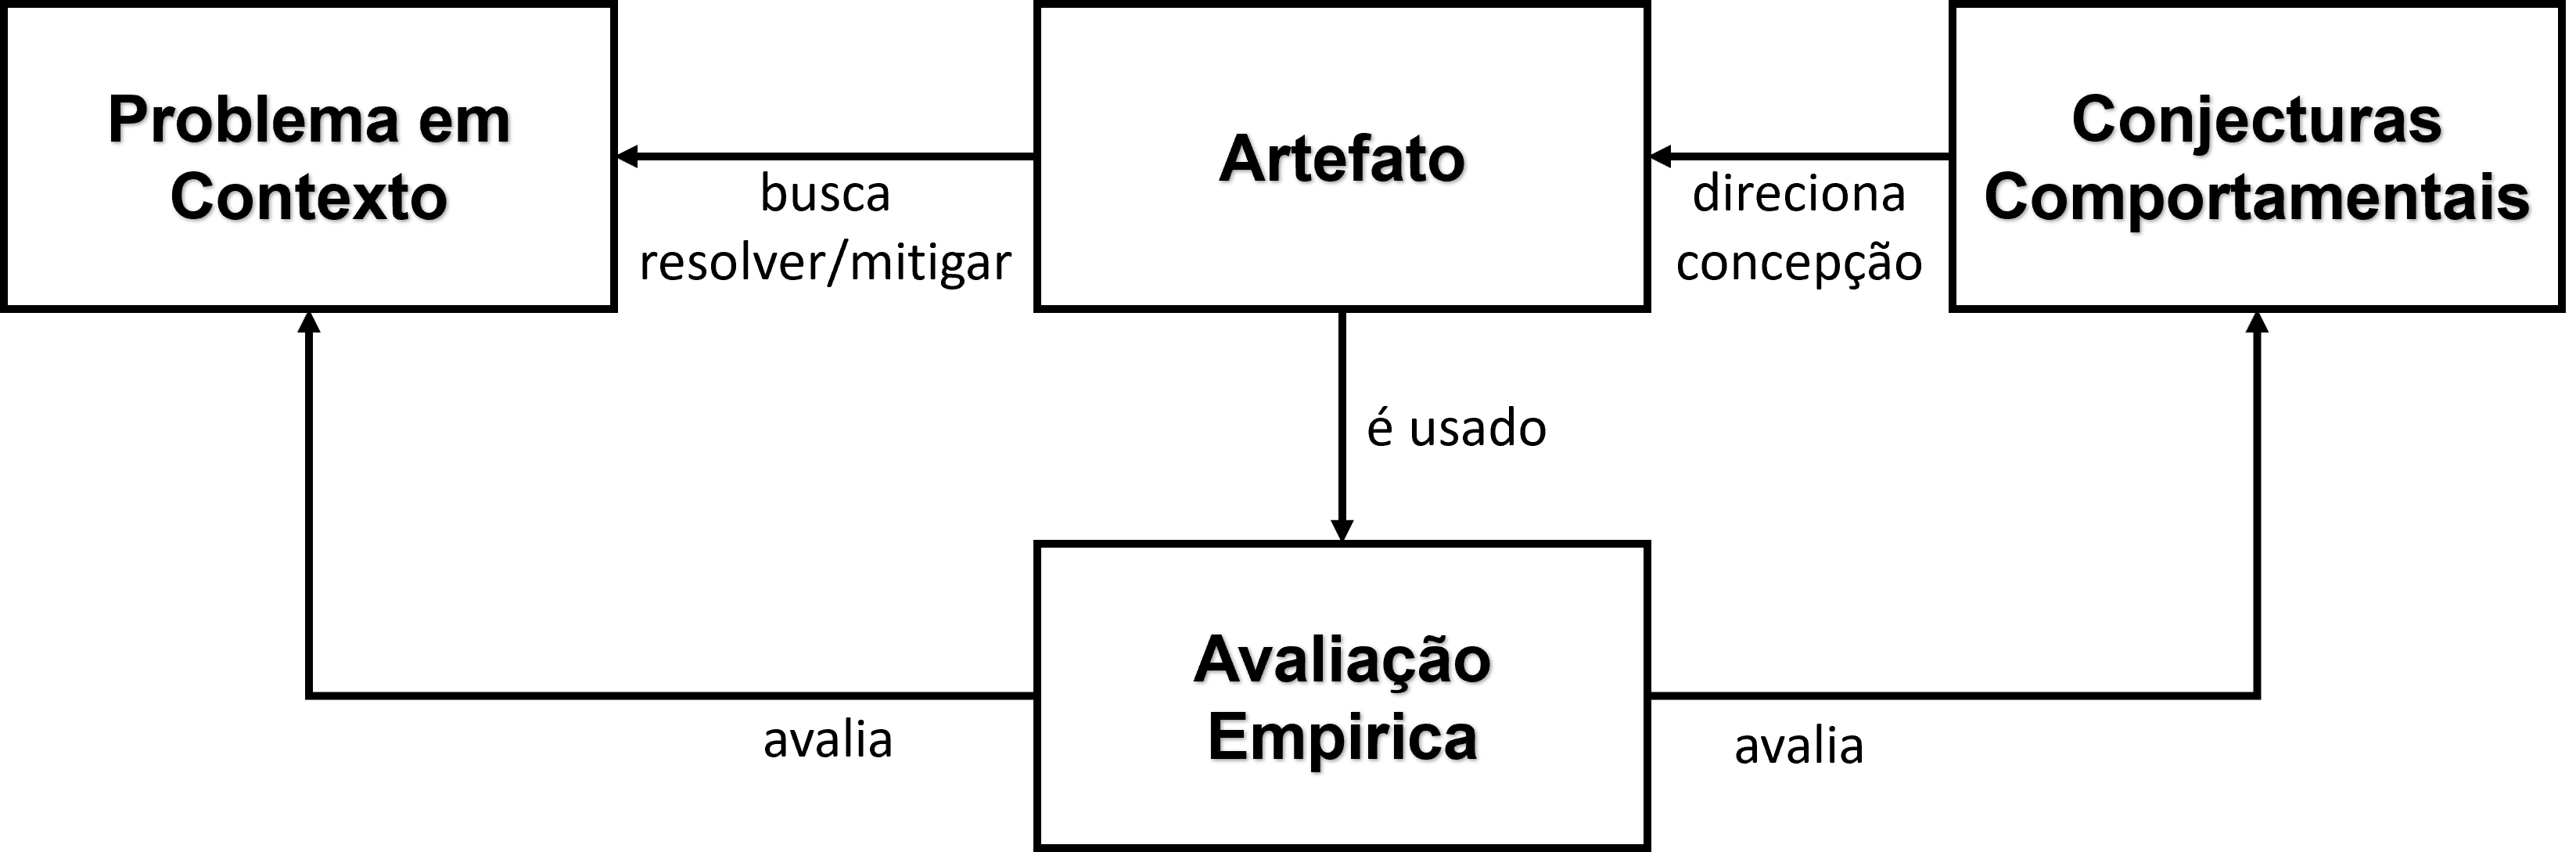
\includegraphics[width=0.5\linewidth]{Images/dsr pimental.png}
    \caption{Elementos centrais do Model-DSR. Baseado em \citep{pimentel2023}}
    \label{fig:dsrmodel}
\end{figure}

O modelo também propõe um diagrama que explicita de forma resumida as conexões entre teoria, problema, solução e contexto. Esse diagrama, junto com sua explicação no formato de texto, é adotado em vários trabalhos do meu grupo para definir a pesquisa que está sendo feita. Exemplos foram dados por \citet{pimentel2019dsr} e \citet{pimentel2023}.

Ao destacar a produção de conhecimento científico como elemento central da DSR, o MODEL-DSR contribui para diferenciar claramente pesquisa de desenvolvimento tecnológico. Ele é especialmente adequado a pesquisas aplicadas em educação mediada por tecnologia, promovendo o rigor metodológico e a relevância prática.

\subsection{Framework de Pesquisa em Tecnologia da Informação}

\citet{march1995design} propuseram um framework bidimensional (ver \autoref{tab:marchsmith}) para pesquisas em Tecnologia da Informação que distingue entre tipos de artefatos produzidos e atividades de pesquisa realizadas. Os artefatos incluem:
\begin{itemize}
    \item \textbf{Construtos}: são os conceitos que formam a linguagem da área de estudo, usados para descrever problemas e formular soluções.
    \item \textbf{Modelos}: expressam relações entre construtos e servem como representacões de situações-problema ou de soluções.
    \item \textbf{Métodos}: são sequências de passos ou algoritmos utilizados para resolver tarefas específicas.
    \item \textbf{Instâncias}: são realizações concretas de sistemas, ferramentas ou protótipos que demonstram o uso prático dos construtos, modelos e métodos.
\end{itemize}

As atividades de pesquisa compreendem:
\begin{itemize}
    \item \textbf{Construção (build)}: desenvolvimento dos artefatos para um objetivo específico, demonstrando sua viabilidade.
    \item \textbf{Avaliação (evaluate)}: análise sistemática do desempenho dos artefatos em função de métricas e critérios estabelecidos.
    \item \textbf{Teorização (theorize)}: construção de explicações que descrevem como e por que os artefatos funcionam em seu ambiente.
    \item \textbf{Justificativa (justify)}: verificação empírica ou formal das teorias propostas, com base em evidências.
\end{itemize}

Esse framework contribui para organizar e avaliar as pesquisas em TI segundo seu tipo de contribuição, facilitando a compreensão e a comunicação dos resultados científicos.

\begin{table}[hbt]
    \centering
    \begin{tabular}{|c|c|c|c|c|}
    \hline
       & Construção & Avaliação & Teorização & Justificativa  \\    \hline
    Construtos &&&&\\     \hline
    Modelo &&&&\\    \hline
    Método &&&&\\    \hline
    Instâncias &&&&\\    \hline
    \end{tabular}
    \caption{O \textit{Framework} de pesquisa em tecnologia da informação proposto por \citet{march1995design}}
    \label{tab:marchsmith}
\end{table}

Além disso,  \citet{hevner2004design} destacam que a contribuição para o corpo de conhecimento científico é um critério essencial para a validade de uma pesquisa baseada em DSR.

\subsection{Como Não Usar  DSR}

A DSR não é uma solução mágica, principalmente não é uma resposta para ser dada no final de uma tese feita por tentativa e erro. 

O principal problema metodológico é o \textit{retrofit}. O candidato, que foi tateando em busca de uma solução para um problema que o agradava, e acabou por esquecer a metodologia, acaba tentando explicar o que fez com uma DSR ``mais ou menos''.

Claro que há uma culpa do orientador, porém quero lembrar que não só o único responsável pela tese é o orientado, como ele é o único que sofre consequências graves pelo seu erro.




\section{A Revisão Bibliográfica}


São dois os objetivos da revisão bibliográfica:
\begin{itemize}
    \item primeiro, ela deve comprovar que o futuro mestre cumpriu bem as fases iniciais da metodologia científica, isso é, o descobrimento e a descrição do problema e a busca de conhecimentos ou instrumentos relevantes ao problema;
    \item realizado isso, ela deve contextualizar o leitor no domínio do conhecimento. 
\end{itemize}

Uma dissertação de mestrado, porém, não é um documento fechado, que tudo explica, mas sim uma revisão dos conceitos do problema e da solução, e um guia para leituras mais detalhadas. 
Elas são similares a artigos de \textit{survey} e deviam, na prática, ser dignas de publicação como tal.

Seus leitores são de dois tipos principais: a banca, que tem alta especialização, e outros pesquisadores que podem buscar a dissertação como referência e modelo de como fazer o trabalho.

A revisão bibliográfica deve ser focada e deve tentar evitar discutir profundamente assuntos não diretamente correlacionados a dissertação.
É importante que a revisão sirva como um guia de leitura dos assuntos, comentado e fazendo ponderações em relação aos documentos citadas.

É costume separar a divisão, possivelmente em dois capítulos, entre a revisão do problema e a revisão das técnicas usadas na dissertação. A abordagem, em geral, é \textit{top-down}, fazendo uma descrição do mais geral ao mais específico.

Na prática, ela não deve ser uma lista de quem disse o quê, mas uma \textbf{revisão global e comparativa do conhecimento}, inclusive com uma visão histórica, e das relações entre aos problemas e propostas analisados.

Nas dissertações onde se resolve um problema específico, esse problema deve ser bem analisado e explicado, e, possivelmente, bem definido, caso não seja definido de forma apropriada na literatura, atendendo ao passo 2 do método científico. 

Finalmente, uma dos objetivos importantes da revisão bibliográfica é fazer uma análise da contribuição de cada texto revisto, de modo a poder contextualizar a contribuição apresentada na dissertação.


\subsection{Revisões Sistemáticas}

Revisões sistemáticas são ferramentas essenciais para a identificação de lacunas no conhecimento e para fundamentar a construção de artefatos na DSR.  \citet{kitchenham2004procedures} definem revisões sistemáticas como um processo rigoroso, transparente e reprodutível de seleção e análise de literatura.

Existem vários modelos similares com estruturas semelhantes que podem ser usados, mas são mais rápidos, como revisões de escopo e revisões rápidas.

A integração de revisões sistemáticas, ou similares, à DSR assegura que a pesquisa se apoie em uma base sólida de conhecimento existente, aumentando sua relevância e contribuição científica.

Para escolher uma forma de revisão, o artigo de \citet{grant2009typology} lista 14 tipos. A partir daí é necessário buscar a descrição da forma mais adequada de fazê-lo. A Linha de Engenharia de Software trabalha há algum tempo com revisões sistematizadas e é possível encontrar não só definições de como devem ser feitas, mas também bons exemplos entre as teses, dissertações e relatórios técnicos do PESC~\footnote{\url{https://cos.ufrj.br/index.php/pt-BR/publicacoes-pesquisa}}

\section{Leituras Adicionais}


O mercado está cheio de livros sobre ``Como fazer uma tese'' e ``Metodologia Científica'' que pouco ajudam. Muitos são voltados para a burocracia da escrita, ensinando quantos centímetros deve ter uma ficha e o formato de uma bibliografia. O problema é bem maior.

Para a área de STEM, esqueça o famoso livro de Umberto Eco, ``Como Fazer uma Tese'', ele é antigo, não é bom para teses de mestrado e doutorado, fala sobre uma ``tesi di laurea'', que é equivalente a um projeto final no Brasil. O livro tem muitos comentários que não se aplicam à engenharia, outras áreas técnicas, e ao Brasil. 

Entre os bons livros que encontrei, estão:
\begin{itemize}
    \item \citet{freitas2001} apresenta um livro prático, de certa forma com uma abordagem similar a este texto, em seu livro \citetitle{freitas2001}. É uma leitura fácil e bastante útil.
\item \citet{woodwell2014} em seu livro \citetitle{woodwell2014} apresenta uma boa introdução à pesquisa e a busca da causalidade, principalmente ligada ao pós-positivismo.
\item \citet{creswell2021projeto} apresentam em \citetitle{creswell2021projeto} uma boa introdução a métodos qualitativos, quantitativos e mistos dentro de vários paradigmas.
\item \citet{Wazla2021} apresenta uma abordagem sobre a metodologia voltada para Computação em seu livro \citetitle{Wazla2021}.
\end{itemize}

Existem outros bons livros no mercado e, possivelmente, seu orientador pode indicar algum.

Se você está interessado em entender melhor como funciona a Ciência, existe uma ampla literatura. 
Para uma visão introdutória e sistemática, recomenda-se a leitura de \citet{chalmers1999o} em sua obra \citetitle{chalmers1999o}, que apresenta e discute o método científico de maneira acessível. 

Um livro  de leitura mais díficil, é \citetitle{Popper1972} de \citet{Popper1972}. 
Já para uma crítica radical à ideia de método fixo na ciência, \citet{feyerabend1975contra} argumenta em \citetitle{feyerabend1975contra} que a ciência avança por vias muitas vezes anárquicas. 
Em outra linha, mas igualmente influente, \citet{kuhn1962estrutura} propõe em \citetitle{kuhn1962estrutura} a noção de paradigmas e revoluções científicas, destacando a descontinuidade no desenvolvimento do conhecimento. Esses três livros compõe uma biblioteca básica e clássica sobre o assunto.

Se a crítica sociológica à ciência te interessa, \citet{collins1993golem} desconstroem o ideal de objetividade científica em \citetitle{collins1993golem}, mostrando como práticas cotidianas e falhas estão presentes até nos experimentos mais renomados, principalmente por meio de estudos de caso. 
De maneira ainda mais provocativa, \citet{latour1987science} examina em \citetitle{latour1987science} como o conhecimento científico é realmente produzido, destacando as redes de atores, laboratórios, disputas e negociações que tornam uma ideia aceita como ``fato''. Ao invés de tratar a ciência como um corpo fixo de verdades, a obra propõe acompanhar a ciência ``em ação'', antes que seus resultados sejam estabilizados. Essa abordagem inaugura os chamados Science and Technology Studies (STS), rompendo com a imagem idealizada de método científico. 
Na mesma direção crítica, \citet{davis1990sonho} refletem sobre os limites da matematização do mundo e a influência do racionalismo cartesiano em \citetitle{davis1990sonho}, questionando se a matemática é descoberta ou invenção, e como ela molda — ou distorce — nossa compreensão da realidade.
\chapter{Ambiente Universitário}

É importante participar do ambiente universitário. Vá sempre a sua universidade, encontre seus colegas. Vá ao laboratório. Assista a seminários. Troque artigos.


Você não pode faltar de jeito nenhum aos seguintes eventos:
\begin{itemize}
    \item 	Eventos promovidos por seu orientador
    \item 	Eventos promovidos pelo grupo do seu orientador
    \item 	Defesas de tese orientadas por seu orientador
    \item 	Defesas de tese de seus colegas de turma
\end{itemize}

No final, quando você souber qual a formação de sua banca, procure defesas de tese com os mesmos integrantes. Isso ajudará você a conhecer a sua banca.

Seus colegas podem fornecer muita informação para você e você deve fornecer para eles também.

Não se torne um “capacitor” de informações, acumulando-as sem passar para ninguém. O pior tipo de pesquisador é aquele que sabe algo e não divulga.

\chapter{Os Ritos de Passagem}


\begin{center}
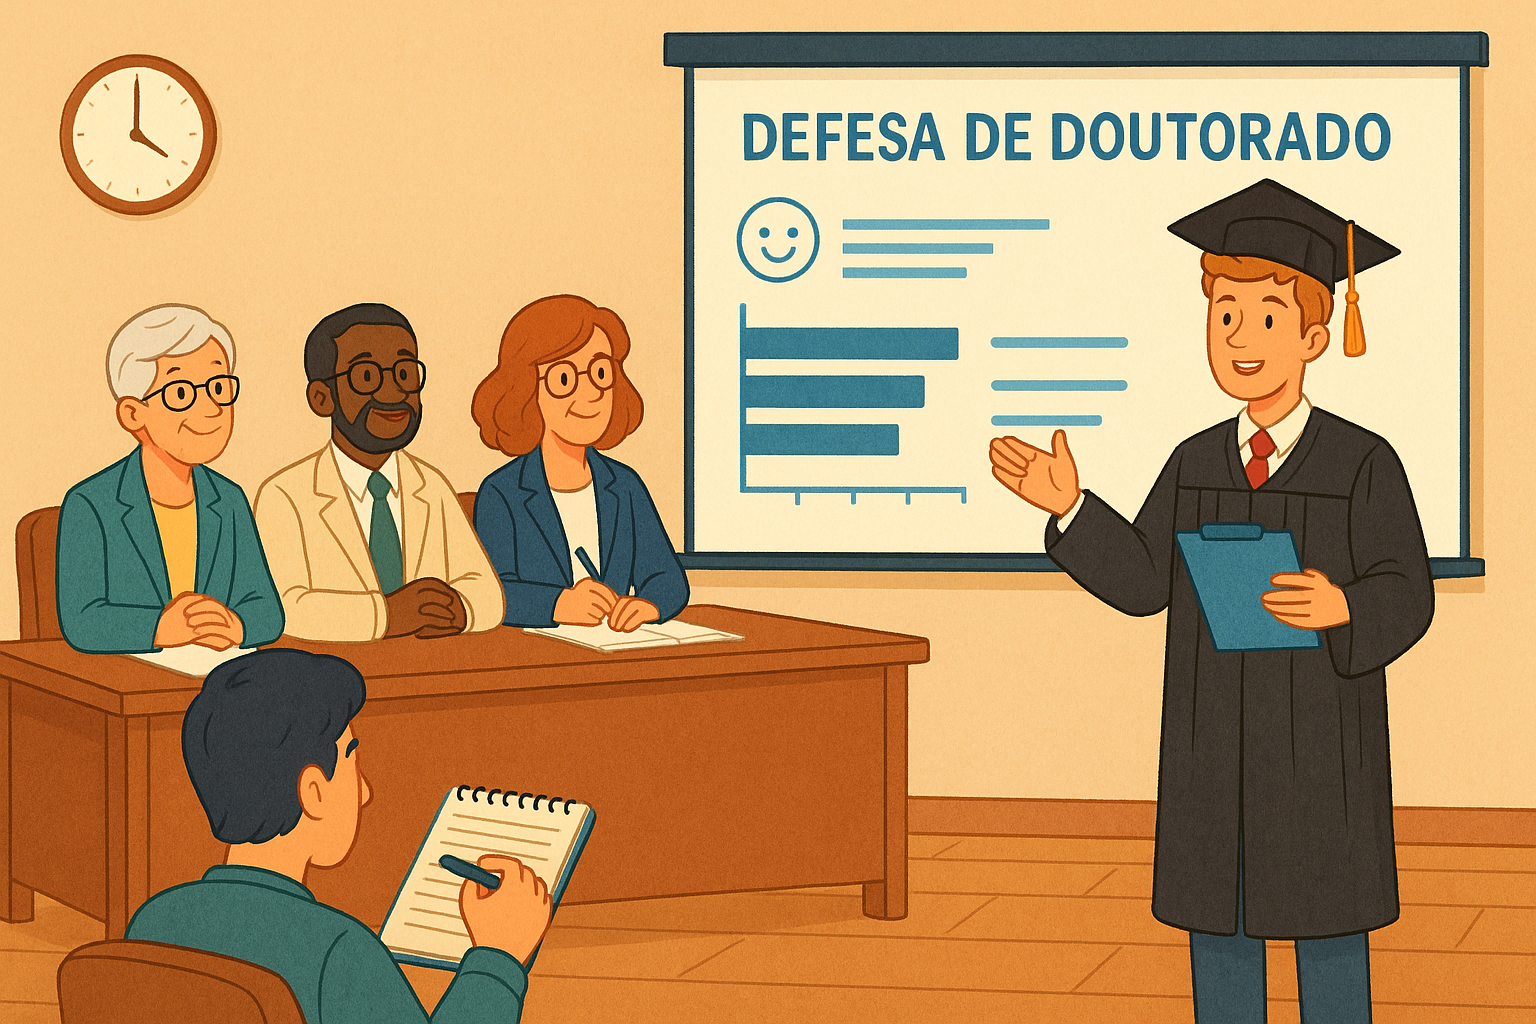
\includegraphics[width=0.5\linewidth]{Images/ritos.png}    
\end{center}
\vspace{0.5cm}

Existem dois importantes ritos de passagem no processo de obter o seu título: a qualificação e a defesa de tese. Normalmente, o aluno passa a ser considerado candidato ao título apenas após um exame de qualificação. 

Praticamente em todos os programas de doutorado, o aluno deve ser aprovado em um exame de qualificação para se tornar um candidato ao doutorado. Já no mestrado, essa obrigação é menos presente\footnote{Para saber mais sobre como as coisas acontecem no PESC/Coppe, veja o \autoref{app:coppedef}}.

\section{O Exame de Qualificação}

O exame de qualificação normalmente busca avaliar 3 quesitos:

\begin{enumerate}
\item	O aluno tem conhecimento suficiente para realizar o doutorado?
\item	O tema de tese conterá uma contribuição original?
\item	O tema de tese é factível?
\end{enumerate}

O momento desse exame varia de programa para programa, e mesmo dentro de um programa, entre os orientadores e alunos. Normalmente, espera-se que se passe um prazo mínimo entre o fim das cadeiras e a realização do exame, para que o aluno tenha um tempo para pesquisar e desenvolver seu tema. 

Em alguns programas, esse exame é feito cedo, tendo mais uma característica de proposta, com muitas suposições. Em outros, ele é feito bem tarde, com o aluno já tendo a tese quase pronta. Esse momento define também o tom do exame.

Um exame mais cedo tem um tom de proposta, e leva muitas vezes a várias discussões, do candidato e da banca, para onde a tese deve se direcionar, que oportunidades são mais claras, e que teorias e métodos podem ser usados. Apesar de eu usar aqui a palavra discussão, deve ser visto como uma discussão colaborativa, onde a banca busca ajudar o futuro candidato. 

Nesse caso, um cuidado a ser tomado é não pensar que o exame de qualificação é como uma tese. Como documento, ele deve ser bem menor; como assunto, ele deve ser focado na proposição e na avaliação de viabilidade. 

Um exame mais tardio tem um tom de pré-defesa, onde a banca já está olhando de forma mais crítica e faz pedidos específicos e orientações mais precisas do que deve ser feito pelo aluno para que ele seja aprovado.

Há locais onde, para o exame ser feito, a tese já tem que estar toda estabelecida e só estejam faltando coisas como partes do experimento final comprobatório ou mesmo uma redação final, funcionando praticamente como um sinal verde para a defesa, ou um sinal de que falta algo importante. 

Para mim, um exame de qualificação de doutorado deve ter pelo menos uma tentativa de solucionar o problema, ou uma investigação na dificuldade de fazê-lo, por meio de tentativas mais ou menos sofisticadas, dependendo do tempo que já foi gasto do prazo da tese.

\subsection{Um Exame para Favorecer o Candidato}

Uma característica do evento de qualificação, seja ele o seminário ou exame, é que a banca é vista como um órgão consultor, ou seja, espera-se que os membros da banca deem sugestões para que o produto final seja melhor. Espera-se que os membros dessa banca participem, mais tarde, da defesa da tese.

Além disso, a banca pode indicar limites, tanto mínimos quanto máximos do que espera da tese ou dissertação. É mais comum que a proposta seja muito ampla, e é costume da banca avisar ao candidato para estreitar seu foco. Raras vezes a banca espera que seja feito mais do que é proposto, mas também é comum que a banca indique caminhos alternativos, ou caminhos adicionais que o candidato pode ou deve seguir, por exemplo, chamando a atenção para um artigo, método ou teoria que o candidato não demonstrou ter conhecimento.

Em todo caso, se espera que esse exame seja para ajudar o candidato, e que, mantendo um padrão de qualidade, permita o que se espera dele na defesa.

\section{A Defesa de Mestrado e Doutorado}

Uma defesa de tese é uma \textbf{apresentação formal} da mesma, na forma de um seminário, pelo candidato, a uma banca de doutores.

Esses doutores são propostos pelo orientador, normalmente, mas não necessariamente, em acordo com o orientado, a um órgão colegiado\footnote{Na Coppe, a CPGP}, que aprova, ou não, a escolha. O orientador escolhe os membros da banca conforme o tema, a experiência e o reconhecimento dos professores convidados, e questões de logística, como disponibilidade nas datas previstas, disponibilidade de verba, etc.

Dependendo do programa, a defesa pode ser realizada na forma presencial, remota ou híbrida. Após a pandemia, e também por dificuldades de verba para viagem de professores, as formas remota e híbrida passaram a ser muito mais aceitas entre os programas.

O candidato deve entregar a sua tese  à banca alguns dias antes, porém esse prazo pode ser menor ou maior de acordo com as circunstâncias e o regulamento\footnote{Na Coppe, o prazo mínimo é 15 dias}. 


\section{Como as Coisas Acontecem na Defesa}

Nesta seção se faz uma narrativa do processo específico da defesa.

\begin{enumerate}
    \item O presidente da banca anuncia o início da defesa, indicando o candidato, o nome da tese, o orientador (normalmente o próprio presidente da banca), a banca (agradecendo a presença) e passa a palavra ao candidato;
    \item O candidato faz a apresentação, na forma de uma palestra de 40 a 50 minutos, onde não pode ser interrompido;
    \item O presidente inicia o processo de comentários e arguição, passando a palavra ao primeiro membro a falar, normalmente ordenando do membro mais externo para o mais interno, sendo os orientadores os últimos a falar;
    \item em sua vez de falar, os membros da banca podem, ou não, fazer perguntas para ser respondidas imediatamente, ou no final de sua fala, ao candidato;
    \item após os membros da banca comentarem a dissertação ou questionarem os candidatos sobre a mesma, a palavra é passada a plateia, que pode ou não se manifestar (normalmente não se manifesta);
    \item o candidato e a plateia se retiram da sala para a banca deliberar (ou banca se retira, principalmente em defesas virtuais);
    \item a banca convoca o candidato e plateia para ler o resultado;
    \item o resultado é lido;
    \item a ata é assinada e se encerra a defesa.
\end{enumerate}

%\needspace{5\baselineskip}
\section{Comportamento e Preocupações do Candidato}

Você deve se preparar para a defesa. No caso de defesa em sala de aula, você deve chegar mais cedo (talvez ir alguns dias antes) para ver como é a sala. 

Deve levar seu próprio computador, um pen-drive de reserva com a apresentação. Não conte com a internet funcionando (Google Slides, por exemplo). Não conte com um computador a sua disposição (apesar de normalmente haver um). 

No caso de defesa remota, você deve ter como fazer a defesa de ``qualquer maneira'', para isso:
\begin{itemize}
    \item Tenha um acesso de internet alternativo. Celulares, por exemplo, podem ser ligados a um computador via USB para funcionarem como modem, ou podem oferecer uma rede wi-fi com a funcionalidade de ``tethering''.
    \item Tenha um computador reserva, pois a casos que o computador dá problema
    \item Verifique antes se câmera, microfone e fone estão funcionando. É essencial que a defesa possua a câmera.
    \item Prepare o celular para backup de câmera, fone e microfone.
    \item Tenha um lugar reserva, pois já aconteceu de ser necessário por falta de luz, internet, etc. 
\end{itemize}

Alguns orientadores fazem uma apresentação prévia\footnote{Não é o meu caso}, outros discutem os slides\footnote{Eu posso rever algumas vezes}. Pergunte o que seu orientador deseja.



\subsection{Slides}

Veja as dicas em \expurl{https://github.com/xexeo/DicasSlidesAcademicos/blob/main/DicasSlidesAcademicos.pdf}{Dicas de Slides Acadêmicos}.

Em especial:
\begin{itemize}
    \item Cuidado com ortografia e gramática;
    \item Cuidado com o tamanho de imagens, principalmente nas letras das imagens, para que sejam legíveis;
    \item Numere os slides, e coloque o total de slides;
    \item Não encha os slides de texto;
    \item Não use corpo de fonte menor que 16;
    \item Tente usar corpo 30;
    \item Não faça show de efeitos especiais, mas use se necessário;
    \item Não se esqueça de dar a atribuição de todas as imagens;
    \item Não se esquecer de agradecer os órgãos financiadores, e
    \item Use as logomarcas institucionais.
\end{itemize}

\subsection{Ao apresentar}

Não fique de costas para a banca lendo os slides. Sua apresentação deve ser de frente para a banca e a plateia, sabendo o que vai falar, por isso deve treinar. Não precisa saber de cor. A \autoref{fig:comparacao-apresentacoes} ilustra esse assunto. 

Nem para apontar para o slide fique de costas para a banca, no máximo fique de lado. Olhe para todos na plateia ao longo da apresentação.

Se preciso, faça anotações sobre o que deve falar, mas não para ler as anotações, mas de forma que elas possam guiá-lo. Os slides devem funcionar da mesma forma.

\begin{figure}[hbt]
    \centering
    \begin{subfigure}[b]{0.45\textwidth}
        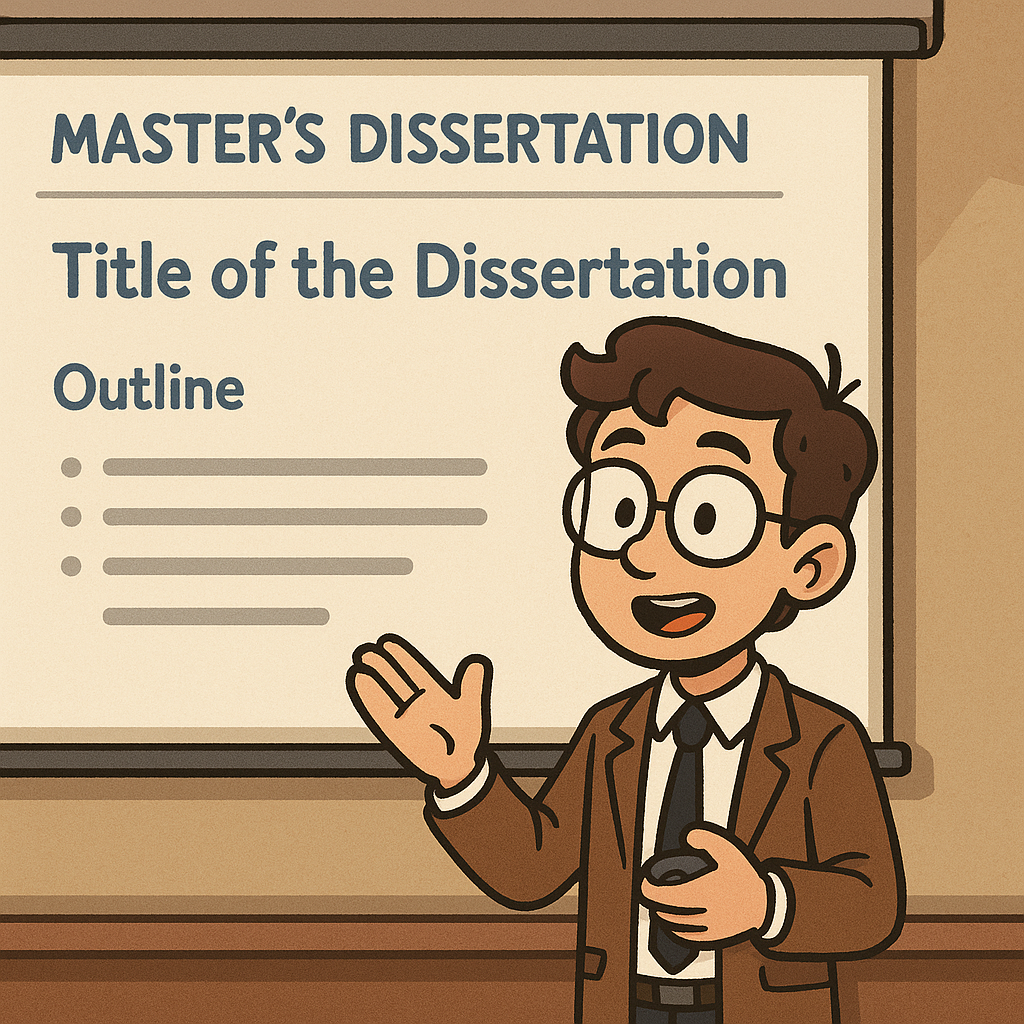
\includegraphics[width=\linewidth]{Images/dandoaulacerto.png}
        \caption{Posicionamento correto do candidato.}
        \label{fig:apresentacao-correta}
    \end{subfigure}
    \hfill
    \begin{subfigure}[b]{0.45\textwidth}
        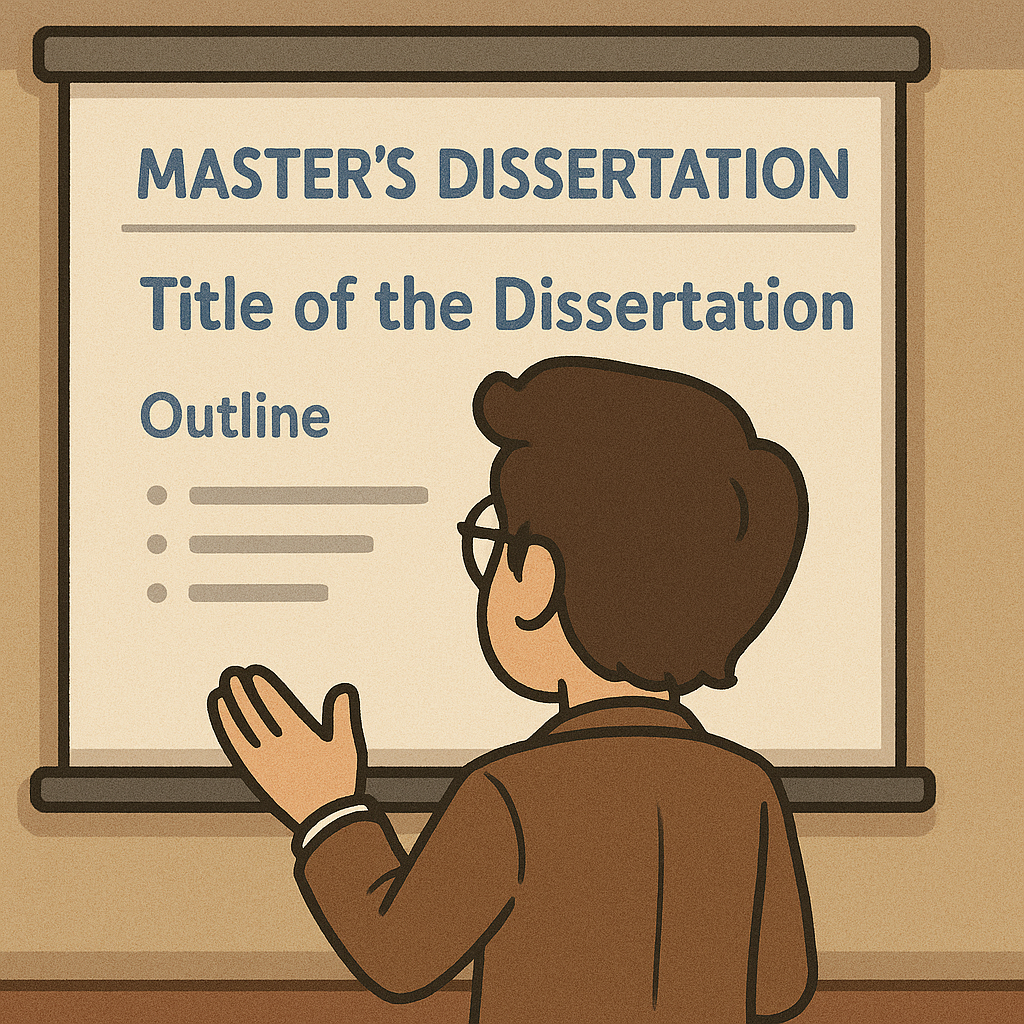
\includegraphics[width=\linewidth]{Images/dandoaulaerrado.png}
        \caption{Posicionamento indevido do candidato.}
        \label{fig:erro-apresentacao}
    \end{subfigure}
    \caption{Comparação entre uma apresentação correta e uma com erro.}
    \label{fig:comparacao-apresentacoes}
\end{figure}



\subsection{Demonstrações de Software}

A melhor forma de demonstrar software é por meio de gravações do sistema funcionando e não rodar diretamente. A experiência prova que é comum que aconteçam problemas de última hora que devem ser evitados. Grave uma utilização e de preferência faça cortes que reduzam os tempos de espera, digitação, etc...

\subsection{Para ficar mais calmo}

É normal ficar nervoso, mas há formas de ajudar a acalmar.
\begin{itemize}
    \item Treine antes, principalmente para fazer a apresentação no tempo. Se você está treinado, vai ficar mais calmo, porque sabe o que tem que fazer.
    \item Tenha com você um copo/garrafa de água, se ficar nervoso, se perder, ou algo assim, pare, respire, tome um gole de água, veja em que ponto está, e então continue com mais calma. O copo de água está ali tanto para matar a sede, como para servir de intervalo sem causar polêmica.
    \item Pelo menos uma vez, no treinamento, grave e veja você apresentando e tente corrigir depois os maus hábitos.
\end{itemize}

\subsection{Durante as perguntas e comentários}

\textbf{Você deve anotar} os que os membros da banca falam. Para isso leve um caderno e caneta. Se quiser gravar (não deixando de anotar), deve pedir autorização. Não anotar é até uma falta de respeito aos comentários da banca. Não é para copiar todas as falas, mas sim deixar um guia para você responder, seja na hora, seja nas correções da dissertação.

Mesmo que o membro da banca fale ``Não precisa anotar porque eu coloquei tudo na dissertação'' ou ``Eu vou te mandar tudo'', anotar é importante para entender o que o membro da banca acha importante, e que perguntas foram feitas.

\section{Os Resultados}

Normalmente os programas admitem três resultados possíveis:
\begin{itemize}
    \item \textbf{Aprovação da dissertação por unanimidade}: significa que você foi aprovado sem modificações de relevância. A banca, e a instituição, ainda esperam que algumas modificações sugeridas sejam feitas, e o aluno tem 30 dias para depositar a versão final no registro e no PESC. O orientador pode ou não auxiliar nas modificações, dependendo da importância delas.
    \item \textbf{Aprovação  somente  após  satisfazer  as  exigências que constam 	 na  folha  de   modificações  no  prazo   fixado  pela  banca    ( não superior  a   uma quantidade de  dias)}: nesse caso, que é comum, será criada uma ata adicional com uma lista de mudanças, e haverá um ou dois indicados para verificar as modificações foram feitas. Normalmente isso significa que a banca reconhece que foi feito um trabalho que quase atingiu o nível necessário do mestrado, mas que precisa de esforços adicionais, ou que precisa de grandes correções de texto. Algumas vezes isso é usado como uma última chance ao candidato e as modificações são de grande monta, podendo resultar na reprovação. Outras vezes é usado como uma forma de garantir um prazo hábil para o candidato fazer mudanças de grande monta no texto, mas considerando que sua aprovação é muito provável.
    \item \textbf{Reprovação da dissertação}: uma ocorrência rara, mas possível, e provavelmente indicada anteriormente pelo orientador sobre sua possibilidade. Indica que o aluno não atingiu o mínimo desejável para o bter o título de mestrado. Já vi algumas reprovações, sendo que os motivos incluíram plágio, experiências não realizadas, e baixa qualidade total do trabalho que tinha sido avisada pelo orientador.
\end{itemize}

Normalmente a reprovação é final, porém eu conheço pelo menos um programa que permite uma nova defesa em um prazo máximo de 6 meses.



\chapter{Resultados}

Só existe uma maneira verdadeiramente honesta de avaliar um trabalho científico: submetê-lo a revisão de seus pares. Por isso existe uma banca de mestrado e doutorado. Por isso cada vez mais é importante publicar seus resultados.

Na forma atual que alunos, professores e programas de pós-graduação são avaliados é impossível imaginar uma tese onde não houve uma publicação. A política correta de um orientador deve ser não permitir a defesa de uma tese que não tenha nenhum artigo publicado. Para isso dou dois motivos: se nenhum trabalho foi apresentado para a publicação, então o aluno não demonstrou interesse, se nenhum trabalho foi aceito, a tese não demonstrou capacidade.

Publicar é responsabilidade do aluno. Cabe ao orientador auxiliá-lo nessa tarefa. Claro que, dependendo da capacidade do orientador na área, ele pode ser a força motriz do artigo. Porém, é importante que o aluno tenha a experiência de conduzir a parte principal do trabalho de publicação.

Uma tese de doutorado tem uma obrigação ainda maior: publicar artigos em revista.

Publique sempre. Antes de acabar a tese, depois de acabar a tese. A única maneira de seu trabalho ficar conhecido e você ser reconhecido é por meio de publicações. Aceite ligeiros atrasos em sua tese (que não interfiram com seu prazo) se for para publicar. Publicar dará pontos em concursos públicos para professor e tornará você conhecido na comunidade.

Ao publicar, não esqueça que os autores são, pelo menos, você e seu orientador. Geralmente o aluno vem em primeiro lugar, mas algumas vezes, principalmente quando a ideia principal vem do orientador, o nome dele vem em primeiro. Publicar sem o nome do orientador é um dos maiores pecados que um aluno pode fazer contra a relação aluno/orientador na área da Computação.

A questão da publicação está se tornando cada vez mais séria no Brasil. Tanto a CAPES quanto as universidades estão avaliando seus pesquisadores principalmente em função da quantidade e qualidade das publicações.

\chapter{Hardware e Software}

Quando comecei a escrever esse guia, ainda havia alunos que chegavam na pós-graduação e não tinham um computador conectado na Internet. Nem posso imaginar que alguém esteja nessa condição hoje em dia.

Porém, seu computador está apto a atender as exigências da sua tese? 

Se necessário, compre um computador novo. Basicamente, verifique que computadores as pessoas do seu grupo utilizam. PCs são mais comuns do que Macs no Brasil e geralmente são utilizados nas áreas de engenharia.




\section{Aplicativos Básicos}

Durante a tese você precisará certamente de um editor de textos, um editor de apresentações e, na maioria esmagadora dos casos de pesquisa, uma planilha eletrônica. O Microsoft Office é uma excelente opção. Muitos alunos conseguem fazer tudo usando apenas os aplicativos da Google, mas é quase impossível formatar uma tese corretamente no Google Docs.

Não gosto do Open Office Write e outras ferramentas livres que tentam imitar o Word e Excel , oferecendo funcionalidades similares, porém em geral de pior qualidade e com sérios problemas de compatibilidade até entre si. Não recomendo o uso dessas ferramentas para o texto da tese.

\subsection{Planilha}

Muitas teses precisam de apresentar alguns resultados na forma de tabelas e gráficos. O programa de escolha genérico é, com larga margem, o Microsoft Excel, com o Google Sheet vindo em segundo lugar. 


Existem, porém, programas melhores que as planilhas para fazer gráficos a partir de números. Gnuplot é um programa livre que, com conhecimento, pode produzir gráficos de alta qualidade. Isso se pode dizer de vários problemas de manipulação matemática (como o Matlab) ou estatística (como o SPSS).
Existem outros software, como o Tableau, que também podem ajudar.


\subsection{\LaTeX}

Atualmente, e isso já variou com o tempo, meu software de escolha para escrever teses e artigos é o \LaTeX, por meio do ambiente colaborativo Overleaf. 

O \LaTeX pode também ser usado em sua máquina. Existem versões open-source e gratuitas do TeX e LaTeX, como o MikTeX, para Windows. 

O importante é que, com qualquer das duas soluçoes, mantenha o versionamento, e consequentemente um backup, no GitHub (ou outra ferramente semelhante).

Recomendo também não manter sua tese em um único arquivo. Arquivos longos tendem a criar problemas de edição. No LaTeX é possível quebrar um arquivo e usar comandos de inclusão em um arquivo principal, o que facilita o trabalho. 

\section{BACKUP!}

Backup deve ser seu deus! 
Vários, todos os dias em vários formatos. Guarde seu trabalho com amigos e com seu orientador. Faça backup dos backups. Em qualquer acidente, o backup o salvará. 

Gaste dinheiro com backup. Não reutilize discos de backup. Se possível, tenha um método para guardar grandes quantidades de informação. Tenha um disco rígido externo. 
Existem vários softwares e serviços de backup disponíveis. 

Outra forma é enviar arquivos para backup em sua conta Google ou outra conta criada especialmente para isso.

Mantenha um backup atualizado, de preferência de forma automática.




\section{Desenhando}

Sua tese deve usar desenhos, os softwares livres são muito bons. O PowerPoint também pode ser usado para fazer desenhos bem decentes.

\section{Programas matemáticos}

Caso vá fazer algum trabalho com matemática, mesmo que vá desenvolver na tese programas próprios, é importante ter um software de referência na área, como MatLab, WolfranResearch Mathematica e MathCad, dependendo das ferramentas que precise.
Programas livres: Scilab (substitui o Matlab). 

Outra opção interessante é usar a linguagem Python e os ambientes matemáticos como Anaconda.

\section{Alternativas}

Muitas vezes é desejável usar um software específico, porém ele é muito caro. Os alunos devem investigar:

\begin{itemize}
    \item Versões de aluguel mensal
    \item Versões acadêmicas
    \item Versões específicas para alunos
    \item Opções mais baratas
    \item Opçoes de software livre
\end{itemize}

Curiosamente, alguns softwares já tiveram uma versão gratuita, ou de comunidade, que ainda pode ser encontrada na rede. Elas não têm mais manutenção. Um caso desse tipo é o Astah. 


{\small
\begin{longtable}{
  >{\raggedright\arraybackslash}p{0.28\linewidth}
  >{\raggedright\arraybackslash}p{0.44\linewidth}
  >{\raggedright\arraybackslash}p{0.24\linewidth}
}
\toprule
\textbf{Software Pago} & \textbf{Alternativas Gratuitas / Livres} & \textbf{Categoria de Uso} \\
\midrule
\endfirsthead

\toprule
\textbf{Software Pago} & \textbf{Alternativas Gratuitas / Livres} & \textbf{Categoria de Uso} \\
\midrule
\endhead

MAXQDA & Taguette, RQDA, QualCoder & Análise Qualitativa de Dados \\
NVivo & CATMA, TAMS Analyzer, Taguette & Análise Qualitativa de Dados \\
ATLAS.ti & Cassandre, QDA Miner Lite & Análise Qualitativa de Dados \\

MATLAB & GNU Octave, Scilab, SageMath & Computação Científica \\
Mathematica & SageMath, Maxima, SymPy & Computação Simbólica \\
Maple & SymPy, SageMath, wxMaxima & Computação Simbólica \\

Tableau Desktop & Google Data Studio, Metabase, Grafana & Visualização e BI \\
Power BI Pro & Apache Superset, Metabase, Redash & Visualização e BI \\
Qlik Sense & KNIME, Orange & Visualização e BI \\

Microsoft Office & LibreOffice, OnlyOffice, Google Docs & Escritório / Produtividade \\
Microsoft Word & LibreOffice Writer, AbiWord, Google Docs & Processamento de Texto \\
Microsoft Excel & LibreOffice Calc, Gnumeric, Google Sheets & Planilhas \\
Microsoft PowerPoint & LibreOffice Impress, Google Slides & Apresentações \\

EndNote & Zotero, JabRef, Mendeley & Gerência Bibliográfica \\
RefWorks & Zotero, BibDesk, JabRef & Gerência Bibliográfica \\

Intel Fortran Compiler & GFortran & Programação Científica \\
Matlab IDE & GNU Octave, VS Code + Extensão & Programação Científica \\
Visual Studio Enterprise & Visual Studio Community, VS Code & IDE / Desenvolvimento \\

SPSS & PSPP, Jamovi, JASP, R & Estatística / Ciências Sociais \\
SAS & R, Python (pandas, statsmodels) & Estatística / Dados \\
GraphPad Prism & SciDAVis, Veusz, R + ggplot2 & Estatística / Visualização \\

\bottomrule
\end{longtable}
}


	\chapter{Trabalhando Comigo}
    
Para trabalhar comigo as seguintes regras são obrigatórias. Aceitar ser meu orientado implica em aceitar essas regras.

\section{Artigo}

\begin{itemize}
    \item Todo aluno de mestrado deve publicar pelo menos um artigo em co-autoria comigo, possivelmente em conjunto com outros alunos.

    \item    Todo aluno de doutorado deve publicar pelo menos um artigo por ano em co-autoria comigo, possivelmente em conjunto com outros alunos.

    \item    Todo aluno de doutorado deve publicar um artigo em revista indexada sobre o seu tema de tese de doutorado em co-autoria comigo (regra da Coppe).

\end{itemize}

\section{Compartilhamento}
\begin{outline}
\1	Todo material da tese deve ser compartilhado comigo, no mínimo para questão de backup dos dados. Você pode compartilhar via \textbf{Google Drive}, \textbf{One Drive} ou \textbf{GitHub}.
\1	Todo o seu código deve estar atualizado em um projeto privado \textbf{GitHub}, compartilhado comigo. O \textbf{GitHub} fornece projetos privados gratuitos para alunos. Eu pago e posso abrir o projeto para você.
\1	Todo o seu texto \textbf{Word} deve estar compartilhado comigo em uma das seguintes ferramentas: \textbf{Google Docs}, \textbf{OneDrive}. Um diretório deve ser compartilhado comigo. Existe uma forma razoavelmente simples de manter os documentos \textbf{Word} com controle de versão no \textbf{GitHub}.
\1	Textos em \LaTeX\  devem usar o \textbf{Overleaf} ou \textbf{GitHub} e serem compartilhados comigo.
\1	Todos os seus dados devem estar em um desses ambientes de compartilhamento: \textbf{GitHub}, \textbf{Google Docs}, \textbf{OneDrive}.
\2	Dados muito grandes devem ser combinados a parte
\2	Melhor ainda se estiverem em todos! Por exemplo, trabalhem no \textbf{Google Docs}, mantenham versões no GitHub e backups de curto no Dropbox.
\1	O status da tese pode ser mantido no \textbf{Trello} ou no próprio \textbf{GitHub}.
\2 Eu disponibilizo um estilo que permite manter o status das tarefas em um documento \LaTeX.
\1	Pesquisas bibliográficas devem ser documentadas no \textbf{Parsif.al} ou em algum documento compartilhado comigo.
\end{outline}

Ou seja, o trabalho todo deve ser compartilhado comigo, por dois motivos:
\begin{itemize}
    \item Os direitos patrimoniais de todo trabalho pertence à UFRJ, não a nós. 
    \item Segurança dos dados. Vários alunos já perderam tudo que fizeram porque seu computador quebrou ou evento semelhante.
\end{itemize}

\section{Entender o que falo, fazer o que digo}

Eu espero que meus alunos entendam o que estou falando. Para isso eles têm que fazer perguntas até entender o que quero. Estou disposto a explicar muitas vezes e de jeito diferente de cada vez. Eu falo rápido, sei muita coisa, uso referências pessoais e científicas de várias épocas, posso achar que falei tudo em uma palavra, e você não entender nada. Pergunte! O máximo que pode acontecer é, em vez de uma resposta de má qualidade, eu mandar você ler um texto de boa qualidade.

Por outro lado, se eu peço fazer algo, não espero precisar explicando cada passo. Principalmente burocracia e coisas que estão em fácil acesso ou uma busca no Google de distância. Se eu digo ``Vá à secretaria'', não me pergunte ``onde é a secretaria?''. Se eu digo ``Submeta a tese no registro da Coppe'', não me pergunte como. São coisas simples que, na verdade, você deveria saber, e estão disponíveis em vários sites e documentos. Além disso, elas mudam com o tempo, e com frequência, logo a informação que eu tenho pode não ser as corretas. Eu espero que você leia e compreenda o texto ``Mensagem a Garcia'', Anexo \ref{chap:garcia}, e preste bastante atenção à sua mensagem. Como orientador, eu quero também tornar você uma pessoa capaz de resolver problemas de forma independente.

Especificamente, eu espero que você, ao longo do tempo, saiba sobre como funciona a vida do aluno e a organização. Principalmente quanto às informações que são passadas explicitamente a você em palestras e documentos na recepção do aluno.

Além disso, eu espero que você me responda rapidamente a perguntas como: qual é o órgão financiador da sua bolsa, qual seu prazo, qual seu DRE, que cadeiras fez, qual sua nota na cadeira, etc. Se você não é capaz de responder essas perguntas básicas, eu realmente me decepciono.



\chapter{O Texto da Tese}

O texto da tese (ou dissertação) é de responsabilidade única do candidato. Claramente, o orientador deve orientar a direção desse texto, mas o responsável único, aquele que será aprovado em função do texto, é o aluno.

Não é função do orientador corrigir o português (ou inglês) dos alunos; ao contrário, como orientador, eu espero que os alunos possuam um português de qualidade. Se seu português é ruim, procure um revisor, seja um amigo ou parente voluntário, seja um profissional que você terá que pagar.

Os alunos de doutorado devem priorizar escrever sua tese em inglês. Os alunos de mestrado devem tentar.

\CoppeWay{Línguas Usadas na Tese}{
Na Coppe o texto pode ser em português, inglês ou espanhol. Outra língua pode ser usada, mas precisa ser autorizada.
}

\needspace{5\baselineskip}
\section{7 Capítulos }
O número místico 7 aparece aqui para definir o número de capítulos da sua tese, que tem normalmente a seguinte estrutura (meus alunos):
\begin{enumerate}
\item	Introdução: incluindo motivação, introdução ao tema, premissas, questões de pesquisa ou hipótese, objetivos e metas, descrição dos próximos capítulos
\item	Revisão do Problema: incluindo áreas relacionadas, de preferência por meio de Revisão ou Mapeamento Sistemático, em formato top-down, do problema mais geral ao mais específico.
\item	Revisão das Técnicas de Solução ou Metodologia: mostrado, de forma top-down, as teorias, técnicas, tecnologias ou metodologias usadas na solução do problema
\item	Proposta de Solução: na forma teórica ou conceitual
\item	Implementação: descrição da arquitetura e detalhes técnicos
\item	Experimentos: incluindo resultados e comentários
\item	Conclusão: incluindo contribuições gerais (melhoria na solução de um problema) e específicas (bibliotecas de código) e trabalhos futuros.
\end{enumerate}


Isso pode ser reduzido para 5 capítulos:
\begin{enumerate}
    \item	Introdução
   \item	Revisão
   \item	Proposta
   \item	Experimentos
   \item	Conclusão
\end{enumerate}

É curioso que devido a uma superstição iniciada por um professor da PUC que era ligado à numerologia e outras coisas místicas, evitamos teses com 6 capítulos, um número que não é de sorte!

\needspace{5\baselineskip}
\section{Uma estratégia de escrita}

A tese, ou dissertação, é uma descrição do seu trabalho. Uma boa estratégia para fazer essa descrição é partir das perguntas 5W2H.

Primeiro faça uma lista do que você fez (What).

A partir dessa lista, pergunte para cada coisa que você fez: por que você fez (Why) e como você fez (How).

Isso permitirá gerar um mapa de tudo que deverá aparecer na sua tese.

Quando falo em mapa, digo de forma abstrata, porém não é má ideia construir um mapa conceitual de tudo isso.

As outras perguntas (Where, Who, When, How Much) são menos importantes nesse caso, mas podem dar ideias de trabalho. Por exemplo, onde você fez alguma mudança no código? Quem foi o idealizador de algum algoritmo que você uso? Quanto poder computacional você precisou usar?

Você também pode pensar em 2 Whats: qual o seu problema, qual o seu trabalho. E depois fazer um raciocínio similar. A Figura a seguir mostra uma esquema de raciocínio.

% TODO: \usepackage{graphicx} required
\begin{figure}[hbt]
    \centering
    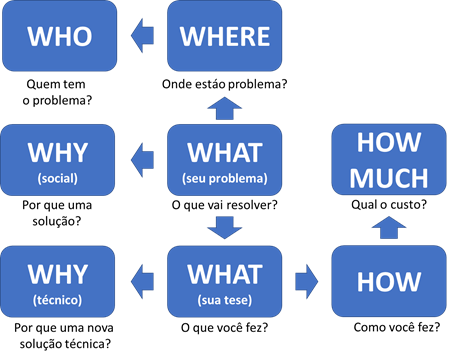
\includegraphics[width=0.7\linewidth]{Images/5w2h}
    \caption{Perguntas que devem ser respondidas antes de iniciar uma tese. Fonte: do autor.}
    \label{fig:5w2h2}
\end{figure}

\section{A tese está no passado}

A tese descreve um trabalho feito. O tempo básico dela é o passado,\textbf{ pretérito perfeito}. Normalmente, o autor não se refere a si, e se o faz, é em um momento onde isso é importante. Em português é comum usar a voz passiva e o sujeito indeterminado, mas a voz passiva não é considerada boa forma em inglês. Nunca usar a primeira pessoa do plural, o ``nós'', que é majéstico, para se referir apenas a você.

O texto, porém, se refere a si mesmo no presente. O presente também é usado para descrever o estado atual das coisas. No texto a seguir, mostramos que a tese ``apresenta'', no presente, trabalhos feitos no passado (``iniciou'',``levou'', ``chegou'') e tem uma proposta de trabalho futuro (``terá'').

\begin{quote}
Esta tese \textbf{apresenta} uma proposta para calcular o número de átomos no universo. Para isso, \textbf{iniciou}-se o processo com uma conta no guardanapo, que \textbf{levou} a diversos experimentos realizados ao longo de dois anos. No final, \textbf{chegou}-se à conclusão de que essa conta será sempre uma estimativa e que a matéria escura ainda \textbf{terá} que ser estimada de forma mais eficaz.
\end{quote}

\needspace{5\baselineskip}
\section{Quanto às figuras}

As figuras ilustrativas de todos os trabalhos dos alunos devem ser feitas, sempre que isso for possível, em linguagens gráficas com uma definição clara\footnote{Fluxogramas são uma linguagem específica, e não um amontoado de caixas e fluxos, que não devem mais ser usados, já que é uma linguagem antiga.}. 

A língua franca da computação atual é UML, que possui uma quantidade de diagramas que ainda podem ser especializados por meio de estereótipos. Outras linguagens podem ser características de áreas específicas, como BPMN e ARIS na descrição de processos de negócio. Deve ficar claro que um gráfico que não é baseado em uma linguagem padronizada, na prática, não significa nada, e passa a ser apenas uma ilustração.

% TODO: \usepackage{graphicx} required
\begin{figure}[hbt]
    \centering
    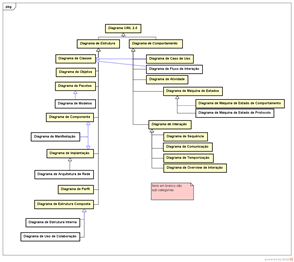
\includegraphics[width=0.7\linewidth]{Images/diagramasuml}
    \caption{Diagramas UML. Fonte: OMG}
    \label{fig:diagramasuml}
\end{figure}






\chapter{O Prazo}

Como todo projeto, uma dissertação ou tese tem que ter um fim.

A COPPE limite o prazo de uma \textbf{dissertação em 3 anos}, mais meio ano de uma possível extensão que, pelo regulamento, não será dada facilmente.

O exame de \textbf{qualificação de mestrado} tem prazo de \textbf{dois anos sem extensão possível}.

O limite de uma \textbf{tese é de 5 anos}, com possível \textbf{extensão} (que novamente provavelmente não será dada) \textbf{de 1 ano}, com \textbf{o exame de qualificação tendo prazo de 3 anos, sem extensão possível}.

Você deve tentar atingir não os prazos máximos da COPPE, mas sim os prazos das bolas: mestrado 2 anos, doutorado 4 anos.

Sabemos que esses prazos são pequenos e eu sugiro que no máximo se chegue a 2,5 anos e 4,5 anos.

O que acontece se você usa o prazo máximo?

Vamos esquecer, momentaneamente, que você pode PERDER O PRAZO, o que é perder o trabalho de anos. Quais os outros problemas?

Primeiro, o texto sai muito pior do que devia, os experimentos são terminados de forma açodada. A banca vai reclamar muito e provavelmente reprovar com restrições e te dar um dever de casa.

Segundo, a capacidade do orientador ajudar em algo nesses casos (fim do seu prazo) é muito reduzida. Por quê? Porque seu orientador tem outras coisas para fazer no trabalho e uma vida pessoal\footnote{Aconteceu comigo, tive uma doença grave junto com o prazo final de muito alunos, incluindo 6 meses de licença, 50  dias de hospital e uma cirurgia de coração aberto. Conseguimos resolver o problema de todos, mas não foi uma boa experiência para ninguém. } , que inclui outros orientados provavelmente também fazendo a mesma coisa. Isso significa que ele, em especial eu, não vai poder realmente orientar o seu final de tese, o que é muito ruim, mas é o que acontece na prática.

Não é razoável você esperar que depois de ficar 5(3) anos fazendo seu trabalho sem muito interesse, no último instante queira uma dedicação emergencial do seu orientador. Ele estava lá por muito tempo. Pode ser que, algumas vezes, ele consiga essa dedicação, mas também pode ser que não.

Ou seja, o seu risco, como orientado, aluno e candidato ao título cresce quando o prazo está chegando. Cuidado!

\chapter{O Caderno de Pesquisa}

Uma prática que dá muito certo é os alunos manterem um caderno normal, de papel mesmo, como registro de trabalho e reuniões.

Tenha sempre o caderno ao conversar com o orientador.

Anote no caderno tudo que você fez, tudo que vai fazer.

Sei que muitos pensam em fazer isso digitalmente. Não é prático, pois não pode desenhar ou rabiscar no celular com a facilidade que faz no caderno.

Cadernos de pesquisa (ou de laboratório) são uma prática antiga que funciona. Recomendo fortemente.

Também são ótimos para criatividade e para guardar ideias que saem do nada.

Eu gosto de usar cadernos de folha branca ou quadriculada.

\chapter{Alguns sites}

\begin{outline}
\1	\expurl{http://www.phdcomics.com}{Quadrinhos PdDComicas}
\2	Quadrinhos sobre doutorandos nos EUA, sou grande fã dessas tirinhas
\1	\expurl{http://www.dissertationdoctor.com/index.html}{Apoio a Doutorandos}
\2	Apoio a doutorandos
\1	\url{http://www.phinished.org/}
\end{outline}


	\chapter{Piadas de Orientados e Orientadores}

Lembrem que toda piada tem um grau de verdade

\section{O Gênio }

Três sujeitos caminhando lado a lado, na hora do almoço. O orientador, o Bolsista de pós-graduação e o Bolsista de Graduação.

De repente, eles veem uma lâmpada velha, dessas bem antigas, das MIL e UMA Noites. O orientador pega a tal lâmpada e dá uma esfregadinha com a mão...

Logo aparece uma fumaceira e sai um Gênio, daqueles grandes, logo dizendo.... ``Normalmente eu concedo UM desejo, mas já que vocês são três, um para cada um''...

O bolsista de graduação gritou... ``Primeiro eu, primeiro eu !''

--- OK! -- disse o gênio

--- Gênio, quero ir para as Bahamas, ficar por lá com muitas mulheres colocando uvas na minha boca, à beira da piscina do melhor hotel que tiver por lá e sem nenhum tipo de preocupação monetária ou de saúde.

BUUM ! O cara desapareceu.

--- Agora eu! -- gritou o bolsista de pós-graduação

--- Pode falar -- disse o GÊNIO.

--- Seu Gênio, me manda para Honolulu. Quero duas gatas dessas bem gostosas para me acompanhar, ficar fazendo surf o ano inteiro.

BUUM! Lá foi o cara embora para os Mares do Sul.

Então o Gênio falou para o orientador: ``Agora você !''

E este diz:

--- Quero esses dois de volta no laboratório depois do almoço.

Moral da história:

Deixem o orientador sempre falar primeiro.

\section{A Tese do Coelho}

Num dia lindo e ensolarado, o coelho saiu de sua toca com o notebook e pôs-se a trabalhar, bem concentrado. Pouco depois, passou por ali a raposa e viu aquele suculento coelhinho, tão distraído, que chegou a salivar. No entanto, ela ficou intrigada com a atividade do coelho e aproximou-se, curiosa:

--- Coelhinho, o que você está fazendo aí tão concentrado?

--- Estou redigindo a minha tese de doutorado -- disse o coelho sem tirar os olhos do trabalho.

--- Humm .. . e qual é o tema da sua tese?

--- Ah, é uma teoria provando que os coelhos são os verdadeiros predadores naturais de animais como as raposas.

A raposa fica indignada:

--- Ora! Isso é ridículo! Nós é que somos os predadores dos coelhos!

--- Absolutamente! Venha comigo à minha toca que eu mostro a minha prova experimental.

O coelho e a raposa entram na toca. Poucos instantes depois ouvem-se alguns ruídos indecifráveis, alguns poucos grunhidos e depois silêncio. Em seguida o coelho volta, sozinho, e mais uma vez retoma os trabalhos da sua tese, como se nada tivesse acontecido. Meia hora depois passa um lobo. Ao ver o apetitoso coelhinho tão distraído, agradece mentalmente à cadeia alimentar por estar com o seu jantar garantido. No entanto, o lobo também acha muito curioso um coelho trabalhando naquela concentração toda. O lobo então resolve saber do que se trata aquilo tudo, antes de devorar o coelhinho:

--- Olá, jovem coelhinho. O que o faz trabalhar tão arduamente?

--- Minha tese de doutorado, seu lobo. É uma teoria que venho desenvolvendo há algum tempo e que prova que nós, coelhos, somos os grandes predadores naturais de vários animais carnívoros, inclusive dos lobos.

O lobo não se contém e cai na gargalhada com a petulância do coelho.

--- Apetitoso coelhinho! Isto é um despropósito. Nós, os lobos, é que somos os genuínos predadores naturais dos coelhos. Aliás, chega de conversa...

--- Desculpe-me, mas se você quiser eu posso apresentar a minha prova. Você gostaria de me acompanhar à minha toca?

O lobo não consegue acreditar na sua boa sorte. Ambos desaparecem toca adentro. Alguns instantes depois se ouvem uivos desesperados, ruídos de mastigação e ... silêncio. Mais uma vez o coelho retorna sozinho, impassível, e volta ao trabalho de redação da sua tese, como se nada tivesse acontecido... Dentro da toca do coelho vê-se uma enorme pilha de ossos ensanguentados e pelancas de diversas ex-raposas e, ao lado desta, outra pilha ainda maior de ossos e restos mortais daquilo que um dia foram lobos. Ao centro das duas pilhas de ossos, um enorme LEÃO, satisfeito, bem alimentado e sonolento, a palitar os dentes.

MORAL DA HISTORIA:

\begin{itemize}
\item Não importa quão absurdo é o tema de sua tese.
\item Não importa se você não tem o mínimo fundamento científico.
\item Não importa se os seus experimentos nunca cheguem a provar sua teoria.
\item Não importa nem mesmo se suas idéias vão contra o mais óbvio dos conceitos lógicos...
\item o que importa é quem é seu orientador...
\end{itemize}

\section{Ditados}
\begin{itemize}
\item	"Tudo que é simples dá mais trabalho que merece"
\item	"Se é estúpido, mas funciona, então não é tão estúpido assim."
\item	"Escopo bom é escopo pequeno"
\item	"Metodologia é função do problema e não o contrário"
\item	"Banca boa é banca de amigos"
\item	"Bibliografia tem de incluir tanto clássicos quanto textos recentes"
\item	"Ciência é Marketing, "venda" sua tese para a banca"
\item	"Cuidado para não misturar autores incompatíveis"
\item	"Planeje seus experimentos antes de colher os dados, senão você pode não ser capaz de analisá-los."
\item	"All models are wrong, but some are useful". - George E. P. Box
\item	"Be regular and orderly in your life so that you may be violent and original in your work" - Flaubert
\item	"Computer Science is no more about computers than astronomy is about telescopes." – Edsger Dijkstra
\item	"Truth is what stands the test of experience." - Albert Einstein
\item	"The more we know, the more we feel our ignorance; the more we feel how much remains unknown"– Sir Humphry Davy
\item	"Science may be described as the art of systematic oversimplification." –  Karl Popper
\item	"The great tragedy of Science – - the slaying of a beautiful hypothesis by an ugly fact." –  Thomas Henry Huxley
\item	"The story of a theory's failure often strikes readers as sad and unsatisfying. Since science thrives on self-correction, we who practice this most challenging of human arts do not share such a feeling. We may be unhappy if a favored hypothesis loses or chagrined if theories that we proposed prove inadequate. But refutation almost always contains positive lessons that overwhelm disappointment, even when [...] no new and comprehensive theory has yet filled the void." –  Stephen Jay Gould (1941-2002), "Bully for Brontosaurus", The Face of Miranda (1991)
\item	"There must be no barriers for freedom of inquiry. There is no place for dogma in science. The scientist is free, and must be free to ask any question, to doubt any assertion, to seek for any evidence, to correct any errors." - Robert Oppenheimer
\item	"To know that we know what we know, and to know that we do not know what we do not know, that is true knowledge." - Copernicus
\item	"I believe there is no philosophical high-road in science, with epistemological signposts. No, we are in a jungle and find our way by trial and error, building our road behind us as we proceed." - Max Born
\item	"Nothing in this world is to be feared... only understood." - Marie Curie
\item	"The fact that some geniuses were laughed at does not imply that all who are laughed at are geniuses. They laughed at Columbus, they laughed at Fulton, they laughed at the Wright brothers. But they also laughed at Bozo the Clown." - Carl Sagan
\item	“A scientist is happy, not in resting on his attainments but in the steady acquisition of fresh knowledge." - Max Planck
\item	"It doesn't matter how beautiful your theory is, it doesn't matter how smart you are. If it doesn't agree with experiment, it's wrong" - Richard Feynman
\item	Crash programs fail because they are based on theory that, with nine women pregnant, you can get a baby a month - Wernher von Braun.
\item	Early to bed, early to rise, work like hell and advertise- Wernher von Braun.
\item	One test result is worth one thousand expert opinions- Wernher von Braun.
\item	Science does not have a moral dimension. It is like a knife. If you give it to a surgeon or a murderer, each will use it differently- Wernher von Braun.
\item	The universe is hostile only when you do not know its laws. To those who know and obey, the universe is friendly- Wernher von Braun.
\item	With every new answer unfolded, science has consistently discovered at least three new questions- Wernher von Braun.
\end{itemize}


\chapter{Mensagem a Garcia}
\label{chap:garcia}
Um texto final para motivar os orientados.

Mensagem a Garcia Elbert Hubbard – fevereiro de 1899

Em todo este caso cubano, um homem se destaca no horizonte de minha memória. Quando irrompeu a guerra entre a Espanha e os Estados Unidos, o que importava aos americanos era comunicar-se, rapidamente, com o chefe dos revoltosos – chamado Garcia - que se encontrava em uma fortaleza desconhecida, no interior do sertão cubano. Era impossível um entendimento com ele pelo correio ou pelo telégrafo. No entanto, o Presidente precisava de sua colaboração, e isso o quanto antes. Que fazer? Alguém lembrou: ``Há um homem chamado Rowan... e se alguma pessoa é capaz de encontrar Garcia, esta pessoa é Rowan''.

Rowan foi trazido à presença do Presidente, que lhe confiou uma carta com a incumbência de entregá-la a Garcia. Não vêm ao caso narrar aqui como esse homem tomou a carta, guardou-a num invólucro impermeável, amarrou a ao peito e, após quatro dias, saltou de um pequeno barco, alta noite, nas costas de Cuba; ou como se embrenhou no sertão para, depois de três semanas, surgir do outro lado da ilha, tendo atravessado a pé um país hostil, e entregue a carta a Garcia. O ponto que desejo frisar é este: Mac Kinley deu a Rowan uma carta destinada a Garcia; Rowan tomou-a e nem sequer perguntou: ``Onde é que ele está?''.

Eis aí um homem cujo busto merecia ser fundido em bronze e sua estátua colocada em cada escola. Não é só de sabedoria que a juventude precisa... Nem de instruções sobre isto ou aquilo. Precisa, sim, de um endurecimento das vértebras para poder mostrar-se altiva no exercício de um cargo; para atuar com diligência; para dar conta do recado; para, em suma, levar uma mensagem a Garcia. O General Garcia já não é deste mundo, mas há outros Garcias. A nenhum homem que se tenha empenhado em levar adiante uma tarefa em que a ajuda de muitos se torne precisa tem sido poupados momentos de verdadeiro desespero ante a passividade de grande número de pessoas ante a inabilidade ou falta de disposição de concentrar a mente numa determinada tarefa... e fazê-la. A regra geral é: assistência regular, desatenção tola, indiferença irritante e trabalho malfeito.

Ninguém pode ser verdadeiramente bem-sucedido, exceto se lançar mão de todos os meios ao seu alcance, para obrigar outras pessoas a ajudá-lo, a não ser que Deus Onipotente, na sua grande misericórdia, faça um milagre enviando-lhe, como auxiliar, um anjo de luz. Leitor amigo, tu mesmo podes tirar a prova. Está sentado no teu escritório, rodeado de meia dúzia de empregados. Pois bem, chama um deles e pede-lhe: ``Queria ter a bondade de consultar a enciclopédia e de fazer a descrição resumida da vida de Corrégio''.

Dar-se-á o caso de o empregado dizer, calmamente: –  ``Sim, senhor'' e executar o que lhe pediste? Nada disso! Olhar-te-á admirado para fazer uma ou algumas das seguintes perguntas:

---  Quem é Corrégio?

---  Que enciclopédia?

---  Onde está a enciclopédia?

---  Fui contratado para fazer isso?

--- E se Carlos o fizesse?

---  Esse sujeito já morreu?

--–  Precisa disso com urgência?

--–  Não seria melhor eu trazer o livro para o Senhor procurar?

–-- Para que quer saber isso?

Eu aposto dez contra um que, depois de haveres respondido a tais perguntas e explicado a maneira de procurar os dados pedidos, e a razão por que deles precisas, teu empregado irá pedir a um companheiro que o ajude a encontrar Corrégio e depois voltará para te dizer que tal homem nunca existiu. Evidentemente pode ser que eu perca a aposta, mas, seguindo uma regra geral, jogo na certa. Ora, se fores prudente, não te darás ao trabalho de explicar ao teu "ajudante" que Corrégio se escreve com ``C'' e não com ``K'', mas limitar-te-á a dizer calmamente, esboçando o melhor sorriso: ``Não faz mal... não se incomode''. É essa dificuldade de atuar independentemente, essa fraqueza de vontade, essa falta de disposição de, solicitamente, se por em campo e agir, é isso o que impede o avanço da humanidade, fazendo-o recuar para um futuro bastante remoto. Se os homens não tomam a iniciativa de agir em seu próprio proveito, que farão se o resultado de seu esforço resultar em benefício de todos? Por enquanto parece que os homens ainda precisam ser dirigidos.

O que mantém muitos empregados no seu posto e o faz trabalhar é o medo de, se não o fizer, ser despedido ou transferido no fim do mês. Anuncia-se precisar de um taquígrafo e nove entre dez candidatos à vaga não saberão ortografar nem pontuar, e –  o que é pior – pensa não ser necessário sabê-lo.

``Olhe aquele funcionário'' -–  dizia o chefe de uma grande fábrica. É um excelente funcionário. Contudo, se eu lhe perguntasse por que seu trabalho é necessário ou por que é feito dessa maneira e não de outra, ele seria incapaz de me responder. Nunca deve ter pensado nisso. Faz apenas aquilo que lhe ensinaram, há mais de 3 anos, e nem um pouco a mais".

``Será possível confiar-se a tal homem uma carta para entregá-la a Garcia?''.

Conheço um homem de aptidões realmente brilhantes, mas sem a fibra necessária para dirigir um negócio próprio e que ainda se torna completamente nulo para qualquer outra pessoa devido à suspeita que constantemente abriga de que seu patrão o esteja oprimindo ou tencione oprimi-lo. Sem poder mandar, não tolera que alguém o mande. Se lhe fosse confiada a mensagem a Garcia retrucaria, provavelmente:

--–  Leve-a você mesmo!.

Hoje esse homem perambula errante, pelas ruas em busca de trabalho, em estado quase de miséria. No entanto, ninguém se aventura a dar-lhe trabalho porque é uma personificação do descontentamento e do espírito da discórdia. Não aceitando qualquer conselho ou advertência, a única coisa capaz de nele produzir algum efeito seria um bom pontapé dado com a ponta de uma bota 44, sola grossa e bico largo.

Pautemos nossa conduta por aqueles homens, dirigente ou dirigida, que realmente se esforçam por realizar o seu trabalho. Aqueles cujos cabelos ficam mais cedo envelhecidos na incessante luta que estão desempenhando contra a indiferença e a ingratidão, justamente daqueles que, sem o seu espírito empreendedor, andariam famintos e sem lar.

Estarei pintando o quadro com cores por demais escuras?

Não há excelência na nobreza de si mesmo; farrapos não servem de recomendação. Nem todos os ricos são gananciosos e tiranos, da mesma forma que nem todos os pobres são virtuosos. Todas as minhas simpatias pertencem ao homem que trabalha, fazendo o que deve ser feito, melhorando o que pode ser melhorado, ajudando sem exigir ajuda. É o homem que, ao lhe ser confiada uma carta para Garcia, toma a missiva e, sem a intenção de jogá-la na primeira sarjeta, entrega-a ao destinatário. Esse homem nunca ficará "encostado", nem pedirá que lhe façam favores.

A civilização busca ansiosamente, insistentemente, homens nessa condição. Tudo que tal homem pedir, se lhe há de conceder. Precisa-se dele em cada vila, em cada lugarejo, em cada escritório, em cada oficina, em cada loja, fábrica ou venda. O grito do mundo inteiro praticamente se resume nisso:

\gxatencao{PRECISA-SE –  E PRECISA-SE COM URGÊNCIA –  DE UM HOMEM CAPAZ DE LEVAR UMA MENSAGEM A GARCIA.}




\printindex

\printbibliography
%\bibliography{citados.bib}
\appendix


\backmatter

\end{document}
